\lhead{\begin{tikzpicture}[remember picture, overlay]
    \node [anchor=100,inner sep=0] (imagenIZQUIERDA) at (current page header area.north){
\includegraphics[width=18cm]{19/Img/encabezado.PNG}};
    \end{tikzpicture}}
    \rhead{Nieto-Leal}
    \rfoot{\begin{tikzpicture}[remember picture, overlay]
    \node [anchor=140,inner sep=0] (imagenDERECHA) at (current page footer area.south){
\includegraphics[width=18cm]{19/Img/foot.PNG}};
    \end{tikzpicture}}
    %----------------------------------------------------------------------------------------
    \lfoot{ \thepage}
    % \renewcommand{\labelenumi}{\alph{enumi}.)} 
    %----------------------------------------------------------------------------------------
    %----------------------------------------------------------------------------------------
    %	TITLE SECTION
    %----------------------------------------------------------------------------------------
    
    \setlength{\droptitle}{-5\baselineskip} % Move the title up
    \title{\textbf{Estudio de tiempos y movimientos en el ensamble de un circuito electrónico utilizando diferentes métodos para su optimización }} % Article title
    
     \author{ 
     \textsc{Nieto-Leal, Emiliano }\\ 
    %  Afiliación:
     \texttt{ Instituto Tecnológico de Querétaro } \\ 
     \texttt{Tecnológico Nacional de México } \\ 
     \texttt{Querétaro, México}\\ 
     \texttt{l22140880@queretaro.tecnm.mx} 
     \and 
     \textsc{Ángeles-Hurtado, Luis Alberto}\\ 
    %  Afiliación:
     \texttt{ Instituto Tecnológico de Querétaro } \\ 
     \texttt{ Tecnológico Nacional de México } \\ 
     \texttt{Querétaro, México}\\ 
     \texttt{alb3rt0.ah@gmail.com} 
    }
    
    
    %----------------------------------------------------------------------------------------
    
    % \begin{document}
    
    % Print the title
    \maketitle
    \thispagestyle{fancy}
    
    %----------------------------------------------------------------------------------------
    %	ARTICLE CONTENTS
    %----------------------------------------------------------------------------------------
    
    % \section*{Resumen}
    % \textit{Palabras clave:}
    % El resumen (ancho de página) deberá contener entre 100 y 200 palabras tipo Adobe Devangari 11 puntos.
    
    \begin{abstract}
    \noindent 
    El resumen (ancho de página) deberá contener entre 100 y 200 palabras tipo Adobe Devangari 11 puntos.
    
    \end{abstract}
    % 
    % 
    \textbf{\textit{Palabras clave}}: {Tiempo, Movimiento, Medición, Muestreo, Registro y Optimización.}
    % \keywords{First keyword should be the corresponding to the research area according with the authors guide. Maximum of 6 keywords.}
    
    \section{Introducción}
    
    
         En la industria siempre se necesita de una mejora continua, por lo que a la hora de empezar trabajos como en ensamblaje (los cuales requieren de varias piezas y herramientas a utilizar) o para poder acelerar los tiempos de producción y minimizar los movimientos para el trabajo, es necesario que cualquier analista entienda las bases de los métodos diseñados para su estudio, siendo el principal de estos el estudio de tiempos y movimientos.\cite{RAE}
        \\En líneas generales el estudio de tiempos y movimientos es una herramienta que permite el analizar todo aquello que de alguno u otra manera tenga relación o afecte al trabajo que se plantea en el estudio(siendo estos los métodos, materiales, herramientas a usar y las instalaciones donde se trabajara), permitiendo separar todos estos factores para su estudio detallado y así buscar optimizar el trabajo estudiado.
        \\Siendo la optimización no solo el objetivo mas importante de estos métodos sino un concepto que siempre se debe de considerar y procurar en todo momento. Al ser " la selección de una alternativa mejor, en algún sentido, que las demás alternativas posibles"\cite{Pontificia2001}. Sumado al estudio de tiempos y movimientos hay mas metodologías que permiten la optimización de las operaciones, estando tanto los estudios de tiempo, en el cual  se busca obtener el valor esperado de cuanto tiempo tomará realizar una actividad, el muestreo de trabajo el cual con base en una muestra elegida de operadores podemos obtener los valores deseados, y principalmente los sistemas de tiempo predeterminados, los cuales tienen como propósito dividir los trabajos en elementos y que con ayuda de unas tablas podemos calcular y asignar un tiempo para cada uno de estos elementos, de esta manera llegando a obtener el tiempo total de la operación.\cite{EstTrabajo}
        \\Por ello para entender de mejor manera como es que se utilizan diversas metodologías y herramientas relacionadas a optimización de los procesos de fabricación se deberá determinar el tiempo productivo y no productivo que un operario (en este caso un compañero) realizara en relación al ensamblaje de un circuito eléctrico. Con ensamble nos referimos a la unión de varias piezas eléctricas, usando un "Protoboard como base para circuito eléctrico, el cual es un conjunto de componentes eléctricos utilizados en la generación y transmisión de energía eléctrica para un propósito en especifico.\cite{CircElec}
        Por lo que usando diversos metodologías para poder obtener los valores del tiempo productivo de nuestros compañeros, creando un registro histórico de estos valores y así poder realizar una comparación entre los métodos utilizados, para de esta manera no solo obtener mayor experiencia en su uso, también observando cual método se adecua mas para cada situación.
    
    % 
    % 
    \section{Justificación}
    
        A día de hoy debido a los grandes avances en tecnología y a la cercanía del mundo entero debido a herramientas como el internet y las redes sociales han generado una globalización que ha afectado a cualquier tipo de mercado existente, considerando un nuevo cambio industrial general. 
         \\Conforme han pasado los años se han dado un consenso que las revoluciones industriales han marcado siempre periodo de transformación tanto económicos, sociales, educativos y organizativos, ocurriendo estas desde el siglo XVII, iniciando con un aumento en la producción mecánica, la generación de producción en masa, creación de servicios digitales y por ultimo la llegada de la 4ta transformación, la cual descrita por Klaus Schwab en el 2016 que "una convergencia entre distintas tecnologías digitales, físicas y biológicas que cambian la forma de vida, de trabajo y de relacionarse los unos con los otros".\cite{4Rev} A día de hoy en base a cada una de estas transformaciones se han generado una gran variedad de manufacturas las cuales dependiendo de cual se use tiene ventajas y desventajas en diversas áreas, siendo en general divididos en 6 tipos distintos de manufactura. \cite{UCSP}
         \\A pesar de la gran cantidad de información generada no se conoce con exactitud la cantidad de industrias que hay en el mundo, se tiene un ranking  general de cuales países son los mas manufacturados, siendo China, Estados Unidos, Japón y Alemania los que ocupan los primeros puestos. En cuanto a México su situación en relación a la manufactura, existiendo en 2019 un aproximado de 579,828 establecimientos dedicados a la manufactura\cite{SEDECO}, generando en 2023 una contribución de \$18,081 millones de dólares, que representa el 17.3\% del PIB nacional.
         \\Por ello es esencial que cualquier producto de la industria manufacturera sea analizado por un buen analista para garantizar que con el uso de sus habilidades de pensamiento pueda utilizar la forma mas óptima de realizar todos los procesos y a su vez sin que estos incumplan cualquier tipo de estandarización o que afecte a la calidad del producto.\cite{Indeed}
    % 
    % 
    \section{Descripción del problema}
        El análisis de tiempos y movimientos es una herramienta útil, pero no solo debe de quedarse ahí, ya que debido a la alta tasa de competitividad es importante mantenerse a la vanguardia de de todo nueva metodología o herramienta que pueda no solo facilitar su trabajo sino también y principalmente generar algún beneficio hacia la compañía para mostrar nuestra eficacia y mantener nuestra posición.
        \\Sin embargo a pesar de que es esencial el mantenerse al día para un analista resulta que este también es el reto más grande que estos poseen, ya que la mayoría de trabajadores en la actualidad crecieron en una época con una tecnología y modo de usarla muy diferentes, como es el caso de las herramientas relacionadas al Internet (IoD), por lo cual al ser bastante complejo varias empresas manufactureras deciden quedarse en lo "clásico", evitando mejoras considerables en aspectos como la ciberseguridad o el manejo de publicidad, mientras que otras empresas que han decidido dar el salto a estos medios cuentan con la desventaja de no haber iniciado en esta era por lo cual su transición a esta pueda afectar directamente a su imagen, haciendo que estas se vean opacadas en las competencias globales.\cite{Novatech}
        \\Por todo ello los estudiantes del Tecnológico Nacional de Querétaro deben de mantenerse a la vanguardia con respecto a sus habilidades tecnológicas y el uso de nuevas herramientas para poder realizar su trabajo de manera adecuada al momento de salir a la industria.
    
    
    %\textbf{*La incógnita científica es el elemento cuya solución incrementa el conocimiento científico.}
    % 
    % 
    \section{Fundamentación teórica}
    
    %Es la parte medular y de mayor discusión, deberá ser la fundamentación de la hipótesis, por tanto se deberá señalar claramente la razón de la suposición y fundamentación de la misma. Únicamente referencias científicas.
    
        Como mencionamos anteriormente las metodologías para la optimización del trabajo son fundamentales a la hora de realizar cualquier trabajo, permitiendo al analista "jugar" con la forma con la que se realizan las cosas y a los operadores se busca encontrar la manera de facilitar los trabajos a realizar, por ello mismo es necesario tener en cuanta la mayor cantidad de formas de realizar una actividad, para así de una manera crítica y objetiva encontrar la forma que mas se adecue al proceso de trabajo a realizar. Por esta razón al buscar generar un registro histórico con las herramientas planteadas podemos conjeturar cual es el método mas útil a la hora de realizar trabajos de ensamble a mano como es el caso del proyecto. Por lo que en síntesis el analista buscara la opción de entre todas las posibles que le genere alguna especie de beneficio en un rasgo en especifico del proyecto, siendo en este caso el método que genere mas ahorro de tiempo.
        \\Para este trabajo utilizaremos diversas metodologías que nos permitan obtener el tiempo productivo e improductivo de un trabajador, para así generar el registro histórico y realizar una comparación entre estos valores para llegar al resultado mas adecuado para nosotros, para esto mismo usaremos el estudio de tiempos y movimientos para analizar las metodologías a utilizar al momento de obtener los valores de tiempos en el ensamble del producto, siendo esta divido en 4 pasos: 
        \begin{enumerate}
        \item Encontrar la forma más económica de hacer el trabajo.
        \item Normalizar los métodos, materiales, herramientas e instalaciones.
        \item Determinar exactamente el tiempo necesario para que una persona competente realice el trabajo con una marcha normal.
        \item Ayudar el aprendizaje del operario en el método nuevo.
        \end{enumerate}

        Por eso mismo iniciaremos realizando un muestreo continuo o una película para así poder detectar el tiempo que se tomará en general realizar el ensamble, y de esta manera obtener los valores de cada uno alumno, pudiendo generar el valor esperado (o media) de tiempos y así con ayuda de un calculo en relación al tiempo invertido en este proceso para saber cual fue el porcentaje del tiempo productivo.
        \\Para esto también se usara los sistemas de tiempos predeterminados (o STP's), en el cual se usarán los Therbligs los cuales son micromoviemientos básicos que se utilizan para cualquier trabajo o actividad importante, los cuales fueron creados para facilitar el estudio de movimientos de los esposos GIlberth que se dividen tanto en eficientes como ineficientes:
            \begin{itemize}
        \item Therbligs Eficientes: Son aquellos micromovimientos que no se pueden eliminar y son esenciales para la realización del trabajo.
            \begin{enumerate}
                \item Alcanzar (AL)
                \item Tomar (T)
                \item Mover (M)
                \item Soltar (SL)
                \item Ensamblar (E)
                \item Desensamblar (DE)
                \item Usar (U)
                \item Preposicionar (PP)
            \end{enumerate}
        \item Therbligs Ineficientes: Son aquellos micromovimientos que no agregan valor al trabajo uy deben eliminarse al realizar un analisis al proceso para optimizar la metodología.
            \begin{enumerate}
                \item Buscar (B)
                \item Seleccionar (SE)
                \item Inspeccionar (I)
                \item Demora evitable (DET)
                \item Demora inevitable (DI)
                \item Colocar en posición (P)
                \item Descansar (DES)
                \item Sostener (SO)
                \item Planear (PL)
            \end{enumerate}
              \end{itemize}
              
        los cuales se usan para llevar acabo cualquier actividad, separando el trabajo en estos elementos y recibiendo valores numéricos en relación al tiempo que se gasta en estos para poder obtener el valor de todo el proceso. Para finalizar utilizaremos el muestreo de trabajo en el cual tenemos como objetivo obtener tanto el tiempo productivo, el estándar y sus tolerancias adecuadas en base a un conjunto de datos obtenidas de una muestra de operarios.
        \cite{EstTrabajo}
     
    % 
    % 
    \section{Hipótesis}
    
    %Es la suposición con fundamento científico relativa a la solución del problema, necesidad o de cómo se aprovecha la oportunidad con la incógnita científica y se fundamenta con: 1. Una suposición (en afirmativo o negativo) y ésta deberá vincularse con: 2. La fundamentación científica que deberá ser precisa 3. Una entidad de comparación para probar la suposición y 4. La variable con que se califica o cuantifica la comparación o se prueba la hipótesis.%

    Desarrollar un proyecto integrador relacionado a la optimización del desarrollo del ensamble de un circuito eléctrico en base a las metodologías y herramientas aprendidas en Estudio del Trabajo II, al realizar el proceso de manera más eficiente retirando todo los pasos innecesarios y permitiendo al estudiante generar una optimización en este y futuros proyectos para un avance en su conocimiento práctico.
    
  %  \begin{itemize}
  %      \item Se debe de identificar claramente la suposición científica
  %      \item Se debe de identificar claramente el fundamento científico
  %      \item Se debe identificar claramente la variable de respuesta
  % \item Se debe identifican claramente las realidades o modelos contrastantes
    %    \item Se debe de establecer las variables asociadas, explicativas o que tienen relación funcional con la variable de respuesta
 %   \end{itemize}
    % 
    
    \section{Objetivo}
    
    %Precisar la acción necesaria para probar la hipótesis. Dicha acción se establece mediante el uso de verbos activos y en infinitivo.
El alumno diseñará, mejorará e integrará sistemas productivos de bienes y servicios aplicando tecnologías para su optimización.
Diseñará, implementará y mejorará sistemas de trabajo para elevar la productividad.
En un plazo menor a seis meses y se plasmara en un proyecto integrador.
    
    \subsection{Objetivos específicos }
    
    \begin{itemize}
    \item Desarrollar una guía de emergencia para analizar la instalación en la que se llevo acabo la experimentación.
    \item Analizar los métodos, materiales, herramientas e instalación utilizada o que se ha de utilizar en la ejecución del ensamble de un circuito electrónico.
    \item Se establecerá la forma más económica de realizar el trabajo.
    \item Normalizar los métodos, materiales, herramientas e instalaciones.
    \item Determinar exactamente el tiempo necesario para que una persona competente realice el trabajo con una marcha normal.
    \end{itemize}
    
    %Son actividades orientadas al cumplimiento del objetivo general. Se establecen con verbos activos en infinitivo. Son parte de la acción encaminada a probar la hipótesis. Éstos deben ser precisos, y en lo posible evitar aspectos metodológicos.
    % 
    % 
    \section{Cuerpo (Metodología, modelo matemático, etc.)}
    
    %Cada estrategia metodológica se establece acorde a cada objetivo, y por tanto deberá ser desglosada precisada y ordenada claramente. En consecuencia cada objetivo que se presentó en forma de verbo en infinitivo deberá determinar una estrategia en forma de adverbio. Ej. Desarrollar…Desarrollo. Son las actividades ordenadas que tienen como finalidad la prueba de la hipótesis. 
    
        Debido a que el objetivo principal de este estudio es la comparación de los valores obtenidos por diversos métodos de optimización, estos en base tanto a su procedimiento como a los valores generados en cada registro histórico, es necesario obtener la metodología que beneficie más al proceso a realizar, por lo que es necesario conocer el funcionamiento de todos las metodologías que se buscan utilizar. 
        
        \subsection{Desarrollo de la guía de plan de Emergencia}

        Plan de emergencia: Un plan de emergencia es descrito como una organización de las acciones, personas, servicios y recursos disponibles para la atención de un desastre, utilizando como base una evaluación previa de riesgos, el manejo de materiales de seguridad y una capacitación de parte de los trabajadores y grupos especiales para el manejo de estos desastres, que pueden generar un riesgo a la salud de los trabajadores.\cite{PlanEmer}

        \subsection{Análisis de los métodos, materiales, herramientas e instalación utilizada en la ejecución del ensamble del circuito electrónico}

        \subsubsection{Planeación}

        Para poder empezar este trabajo es esencial el planear como es que llevaremos acabo todas las actividades a realizar, sobre todo con el manejo del material al ser completamente nueva para la mayoría por lo que debe ser tratado con extremo cuidado, buscando generar una lista de pasos sencilla y bien ejemplificada para que el operador pueda realizar el trabajo de manera adecuada, por ello mismo se debe de utilizar herramientas como las 5's para poder garantizar a la hora de llevar acabo las metodologías planteadas estas se hagan con el mayor orden posible, también considerando los datos necesarios para la creación del plan de emergencia, por el cual se debe de tener conocimiento métrico de las áreas cercanas y todo material usado para protección en los alrededores del área.

     \subsubsection{5's}

     Esta metodología se genero en Japón en 1960 en la empresa de Toyota, en la cual utilizando 5 palabras japonesas con la inicial "S" que tiene relación en la gestión y manejo del área de trabajo, siendo las palabras\cite{5S}:

     \begin{enumerate}
         \item Selección (Seiri): En esta se debe tener solo lo que se necesita en el área de trabajo, en el momento que se necesita para así separar y desechar todo lo que no es útil y tirarlo.
         \item Orden (Seiton): Ordenar los elementos de modo que sea mas fácil de usar y a la vez identificar de modo que cualquiera pueda encontrarlos, tomándolos de la zona especificada, utilizarlos y regresar el elemento a su lugar.
         \item Limpieza (Seiso): Mantener todo tan limpio de modo que sea más fácil de detectar cualquier anomalía que se presente en el área de trabajo, buscando mejorar el ambiente y evitar la generación de fallas y accidentes.
         \item Mantenimiento (Seiketsu): Consiste en mantener el ambiente de trabajo y todo el equipo en condiciones óptimas para el desarrollo de las operaciones requeridas.
         \item Disciplina (Shitsuke): Este es el apego a un conjunto de leyes o reglamentos que rigen toda la organización dentro del área de trabajo, buscando un autocontrol de parte de los trabajadores para que estos generen hábitos beneficiosos al desempeñar sus labores.
     \end{enumerate}

     Con la ayuda de este método podremos desarrollar un diseño para el tapete organizador mucho más balanceado y ordenado, para de esta manera a la hora de obtener los valores de tiempos obtenidos sepamos que se eliminaron ciertos factores que pudieron influir en la demora del operador a través de un manejo y dirección adecuado del material.

\subsubsection{Diagrama de procesos Bimanual}
Esta es una herramienta utilizada en el estudio de movimientos, donde presenta todos los micromovimientos realizados tanto con la mano izquierda como con la mano derecha, para de esta manera buscar eliminar aquellos movimientos innecesarios y realizar cada paso de la actividad de manera eficiente, esta será usada en el sistema de tiempos predeterminados para generar un tiempo estándar en base a tablas de tiempo para cada micromovimiento, las cuales se presentarán a continuación, para posteriormente sumar la holgura obtenida.\cite{EstTrabajo} 

\subsubsection{Desarrollo del sistema de tiempos predeterminado}

        Siendo el primero de estos la medición del tiempo productivo a través del uso de una cámara para generar observaciones (una película) del proceso necesario para ensamblar el circuito y así cada miembro del grupo realice su propia medición en base a la película propia. Para posteriormente generar su separación en movimientos a los cuales se le otorgaran un valor de tiempo y así poder de esta manera obtener el valor esperado para cada ciclo a analizar. 
        Para poder desarrollar este método se requiere generar diversas parejas dentro de las cuales se asignaran roles entre el operador y el analista para de esta manera realizar dos observaciones cada uno de como se debe de llevar acabo el ensamble del circuito, llenando un formato con la información básica del operador como en la figura \ref{fig:tablaReferencia} y así generar una película que nos muestre ese proceso para que al finalizar de esta el miembro que tome el rol del operario deberá pasar lo prueba de calidad del producto, el cual es mover los valores de resistencia del potenciómetro para que se muestre una fluctuación en las lecturas de parte del LCD, realizando el mismo proceso pero ahora con la persona que tomo el rol del analista convirtiéndose en el operario y viceversa.
        \begin{figure}[H]
        \centering
        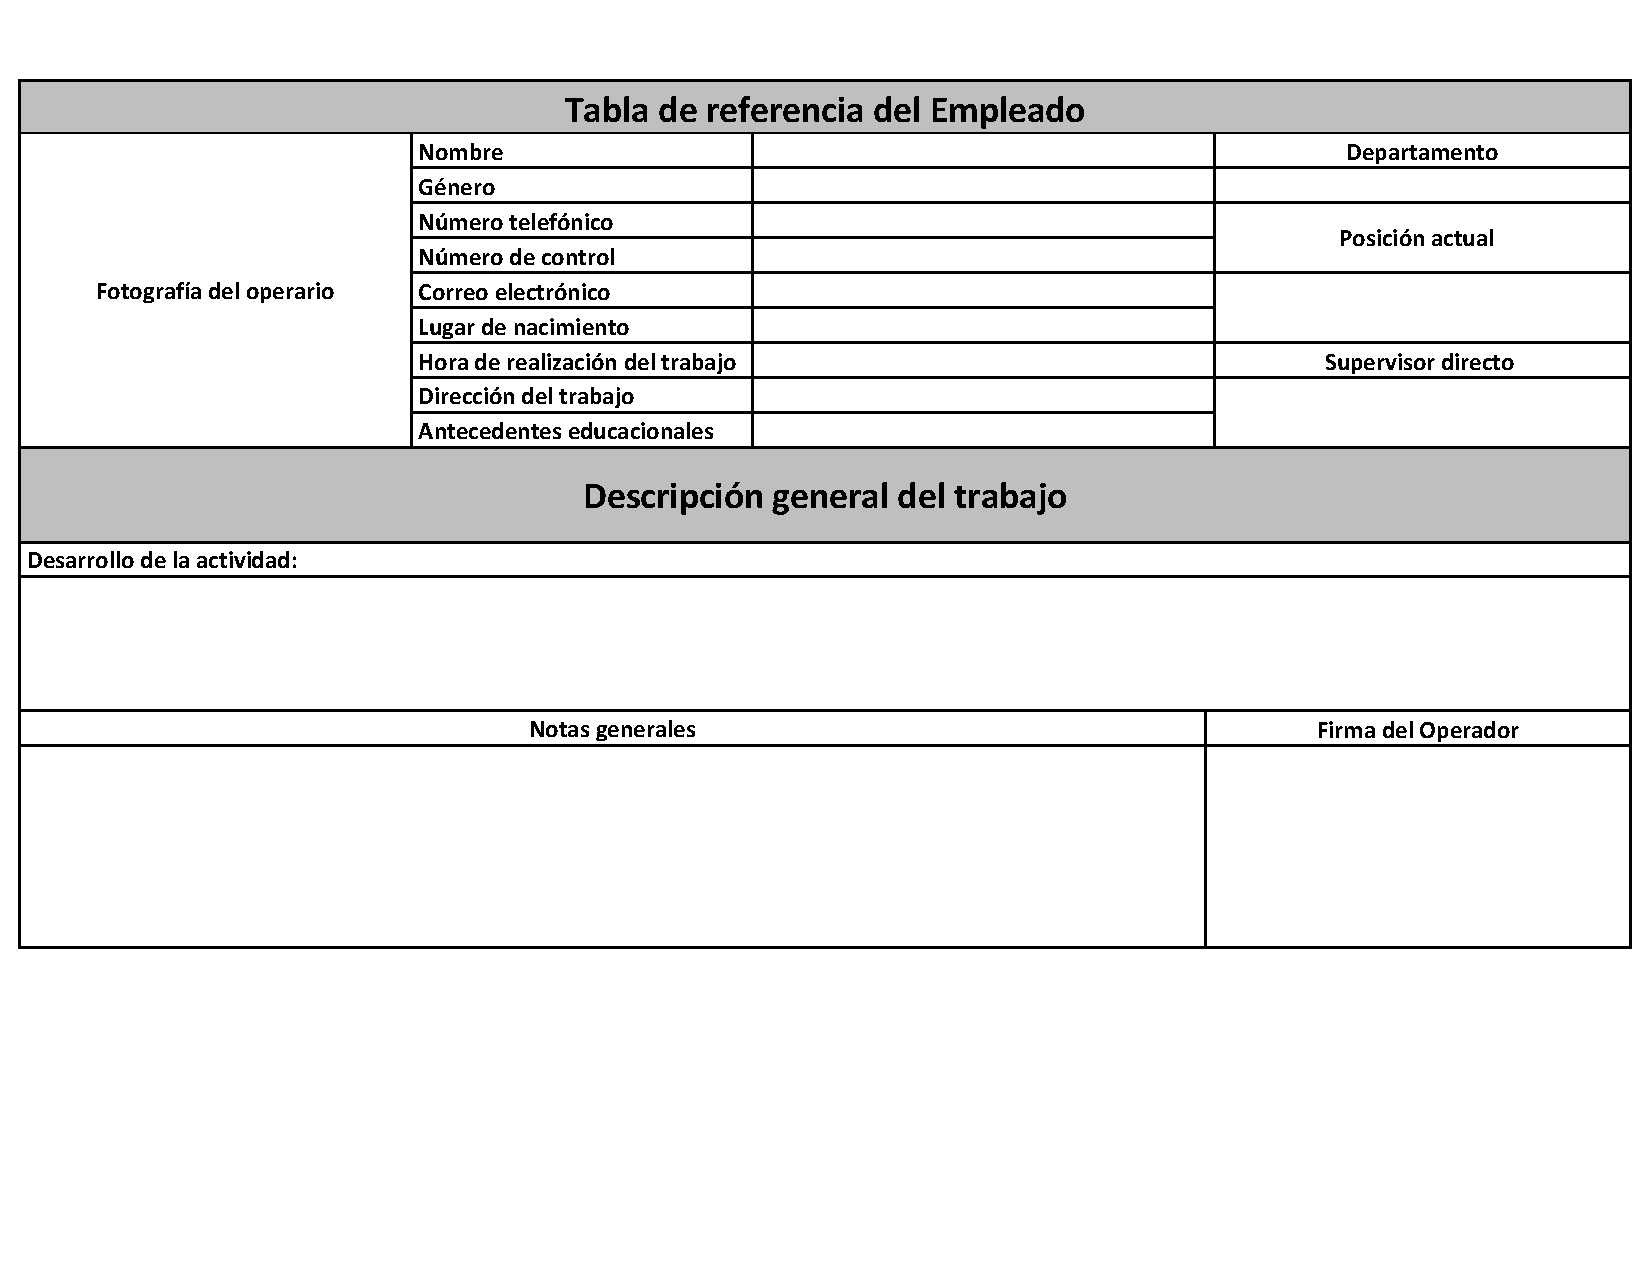
\includegraphics[trim = {1mm 50mm 1mm 1mm},clip,scale=0.3]{19/Img/tablaReferencia.pdf}
        \caption{Hoja de referencia para el operador.}
        \label{fig:tablaReferencia}
    \end{figure}
    MTM-1\\
    Para desarrollar este estudio se decidió utlizar el STP conocido como MTM-1, el cual es el sistema de tiempos predeterminados más comunes y usados, este significa Medicion de Tiempos de Métodos y en este se presentan 10 movimientos básicos con los que se realiza cualquier actividad, siendo los siguientes:
    \begin{enumerate}
    \item Alcanzar (AL)
    \item Mover (M)
    \item Girar (T)
    \item Aplicar presión (AP)
    \item Asir (G)
    \item Colocar (P)
    \item Soltar (SL)
    \item Separar (D)
    \item Movimiento del cuerpo (BM)
\item Movimiento de ojos (ET)
    \end{enumerate}
    Cada uno de estos movimientos poseen su propia tabla de tiempos; estas tablas presentan los TMU son unidades de tiempo que se le otorga a cada movimiento, en cual en base a diversos factores a considerar los cuales se presentarán en las siguientes tablas:
\begin{figure}[H]
        \centering
        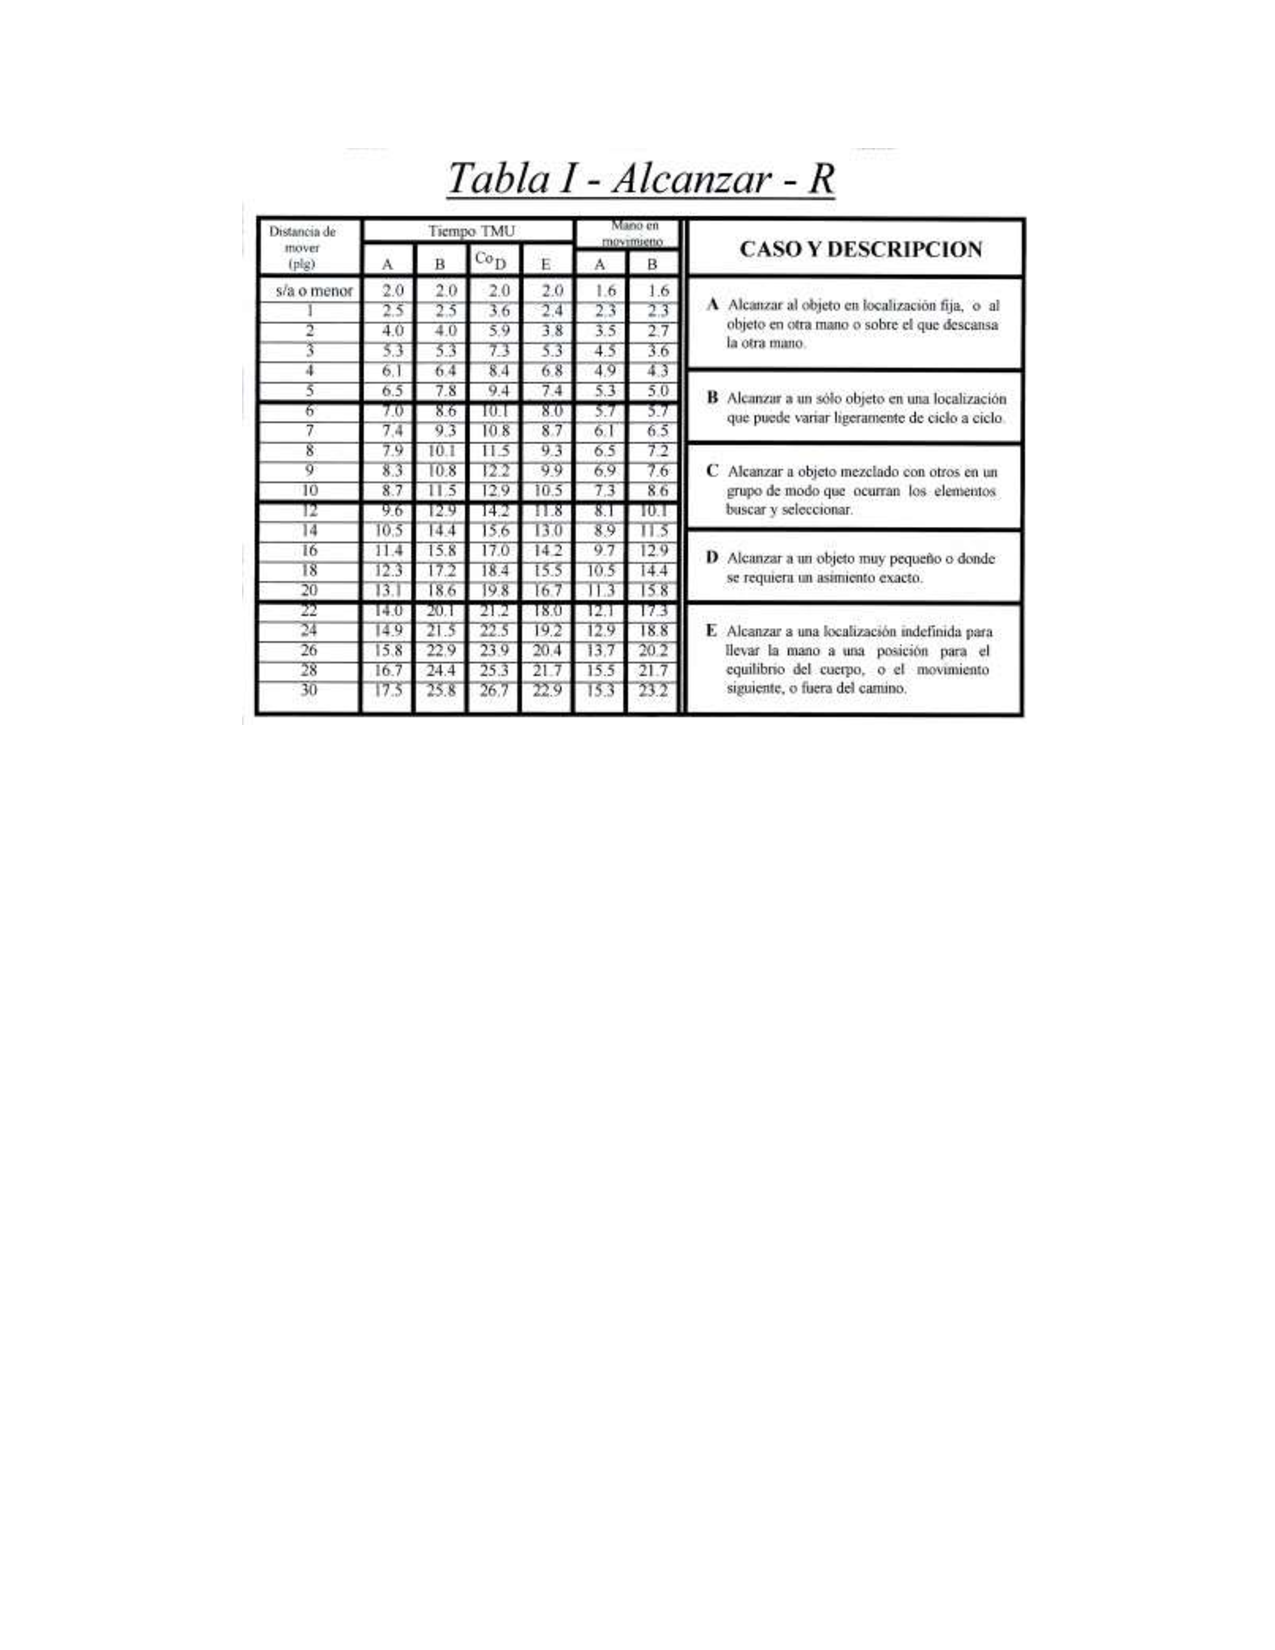
\includegraphics[trim = {42mm 150mm 42mm 24mm},clip,scale=0.6]{19/Img/tablaAlcanzar.pdf}
        \caption{Tabla de tiempos TMU para el movimiento Alcanzar}
        \label{fig:tablaAlcanzar}
    \end{figure}
\begin{figure}[H]
        \centering
        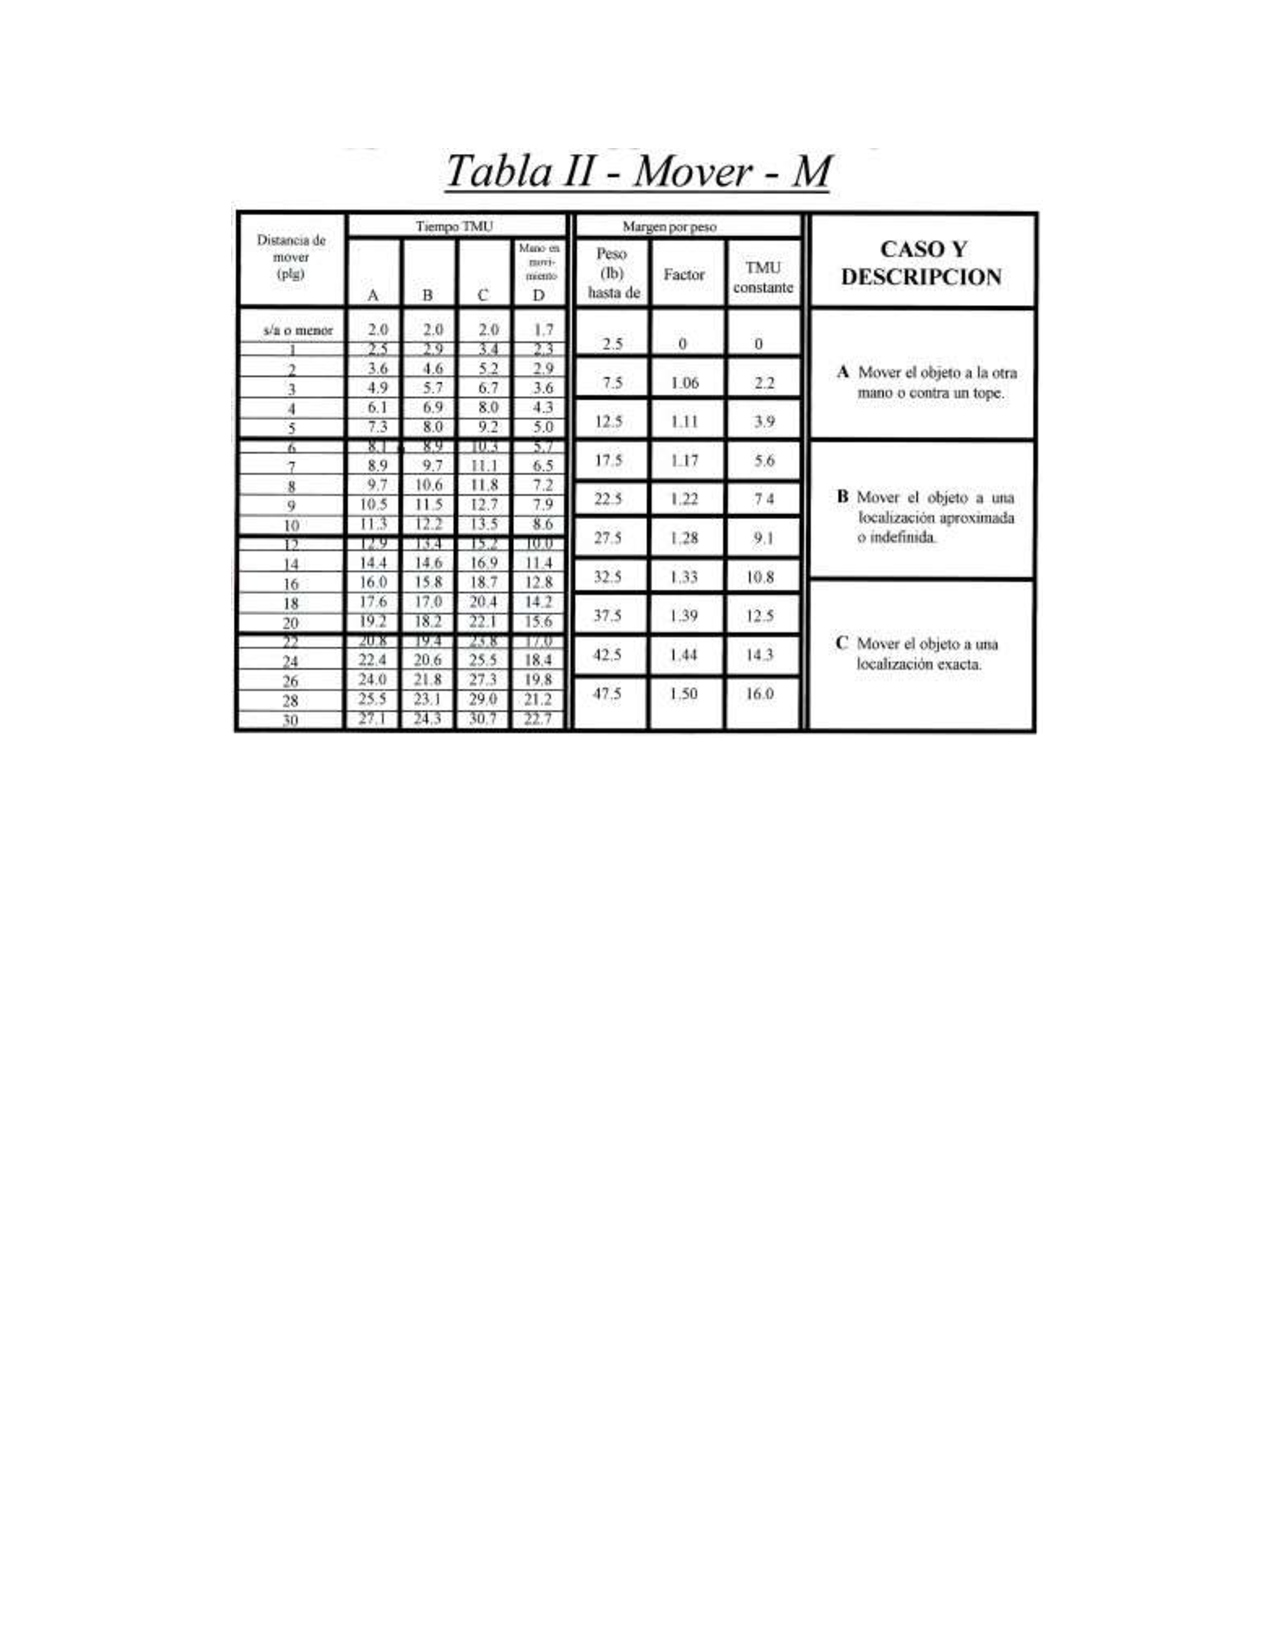
\includegraphics[trim = {42mm 150mm 42mm 24mm},clip,scale=0.6]{19/Img/tablaMover.pdf}
        \caption{Tabla de tiempos TMU para el movimiento Mover}
        \label{fig:tablaMover}
    \end{figure}
    \begin{figure}[H]
        \centering
        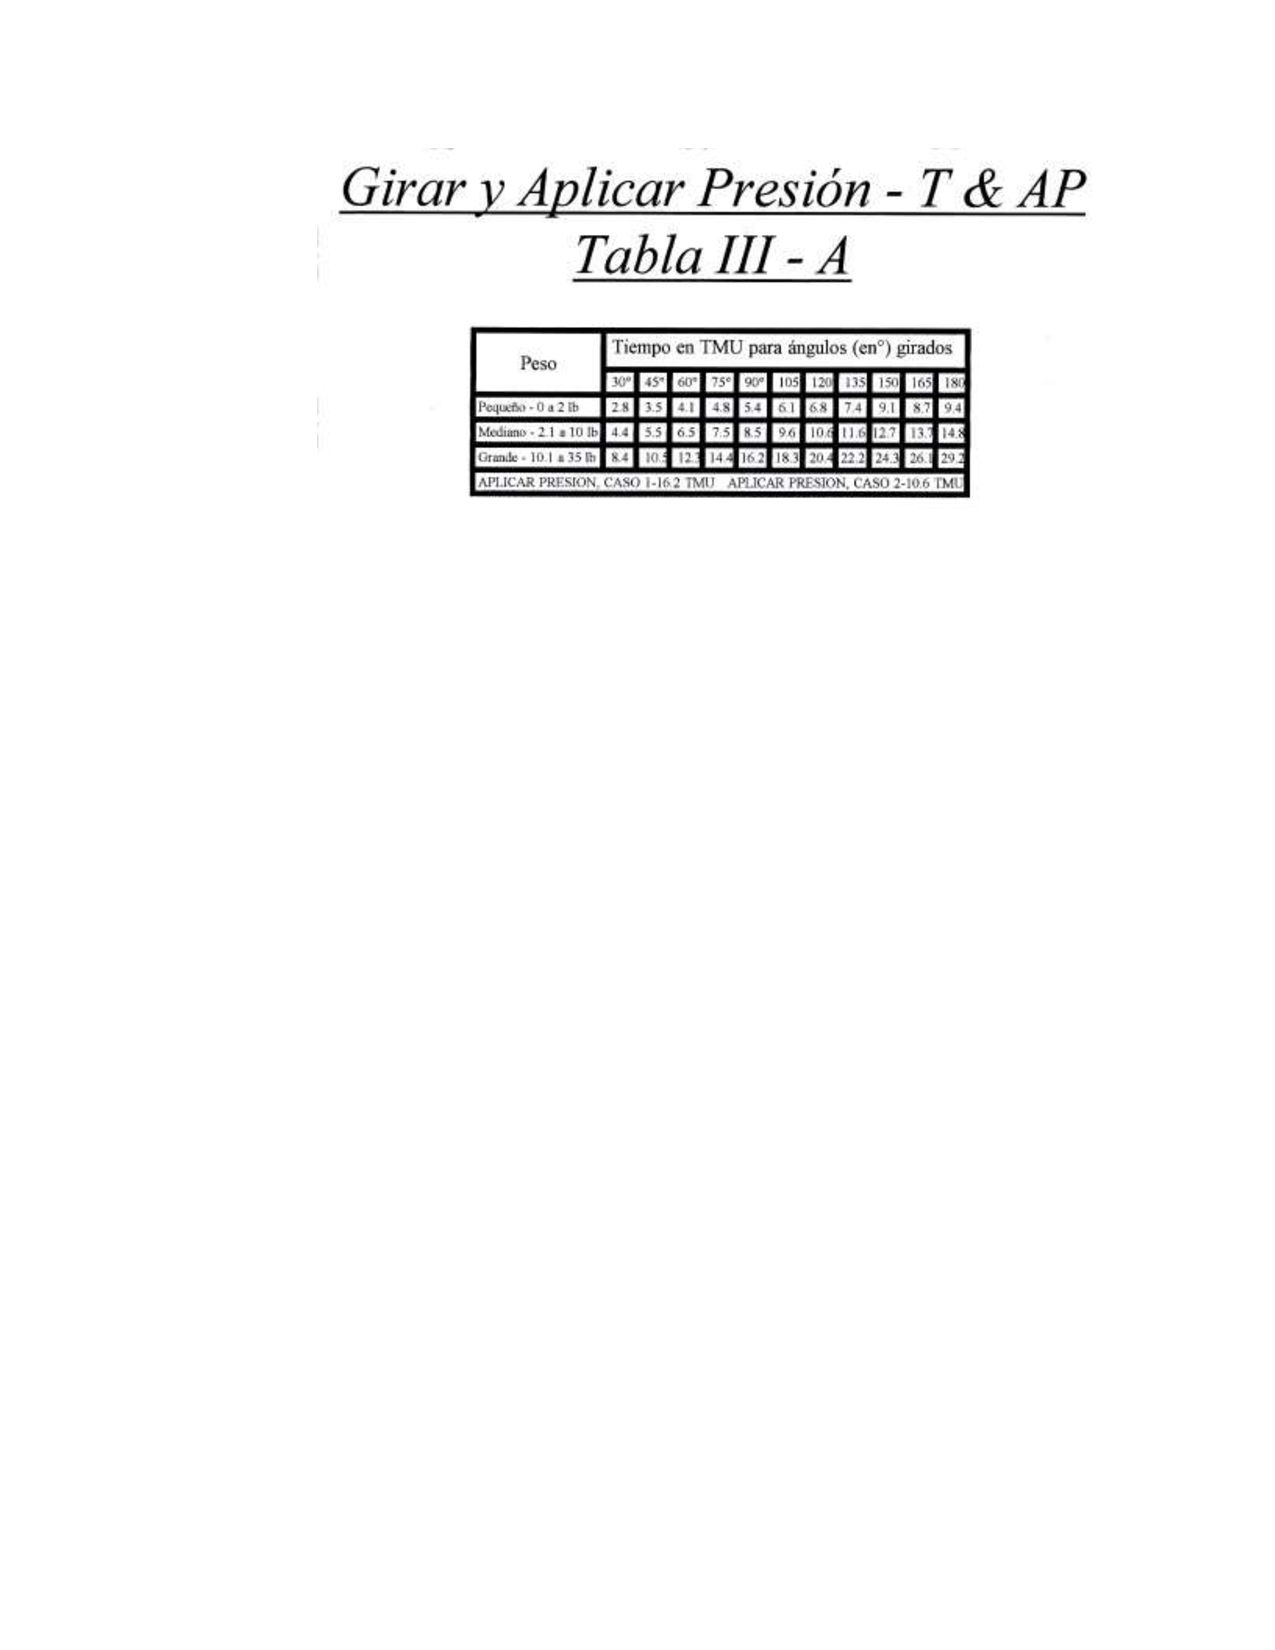
\includegraphics[trim = {42mm 190mm 42mm 24mm},clip,scale=0.6]{19/Img/tablaGirar.pdf}
        \caption{Tabla de tiempos TMU para el movimiento Girar}
        \label{fig:tablaGirar}
    \end{figure}
\begin{figure}[H]
        \centering
        \includegraphics[trim = {42mm 200mm 42mm 24mm},clip,scale=0.6]{19/Img/tablaAplicarPresión.pdf}
        \caption{Tabla de tiempos TMU para el movimiento Aplicar Presión}
        \label{fig:tablaAplicarPresión}
    \end{figure}
        \begin{figure}[H]
        \centering
        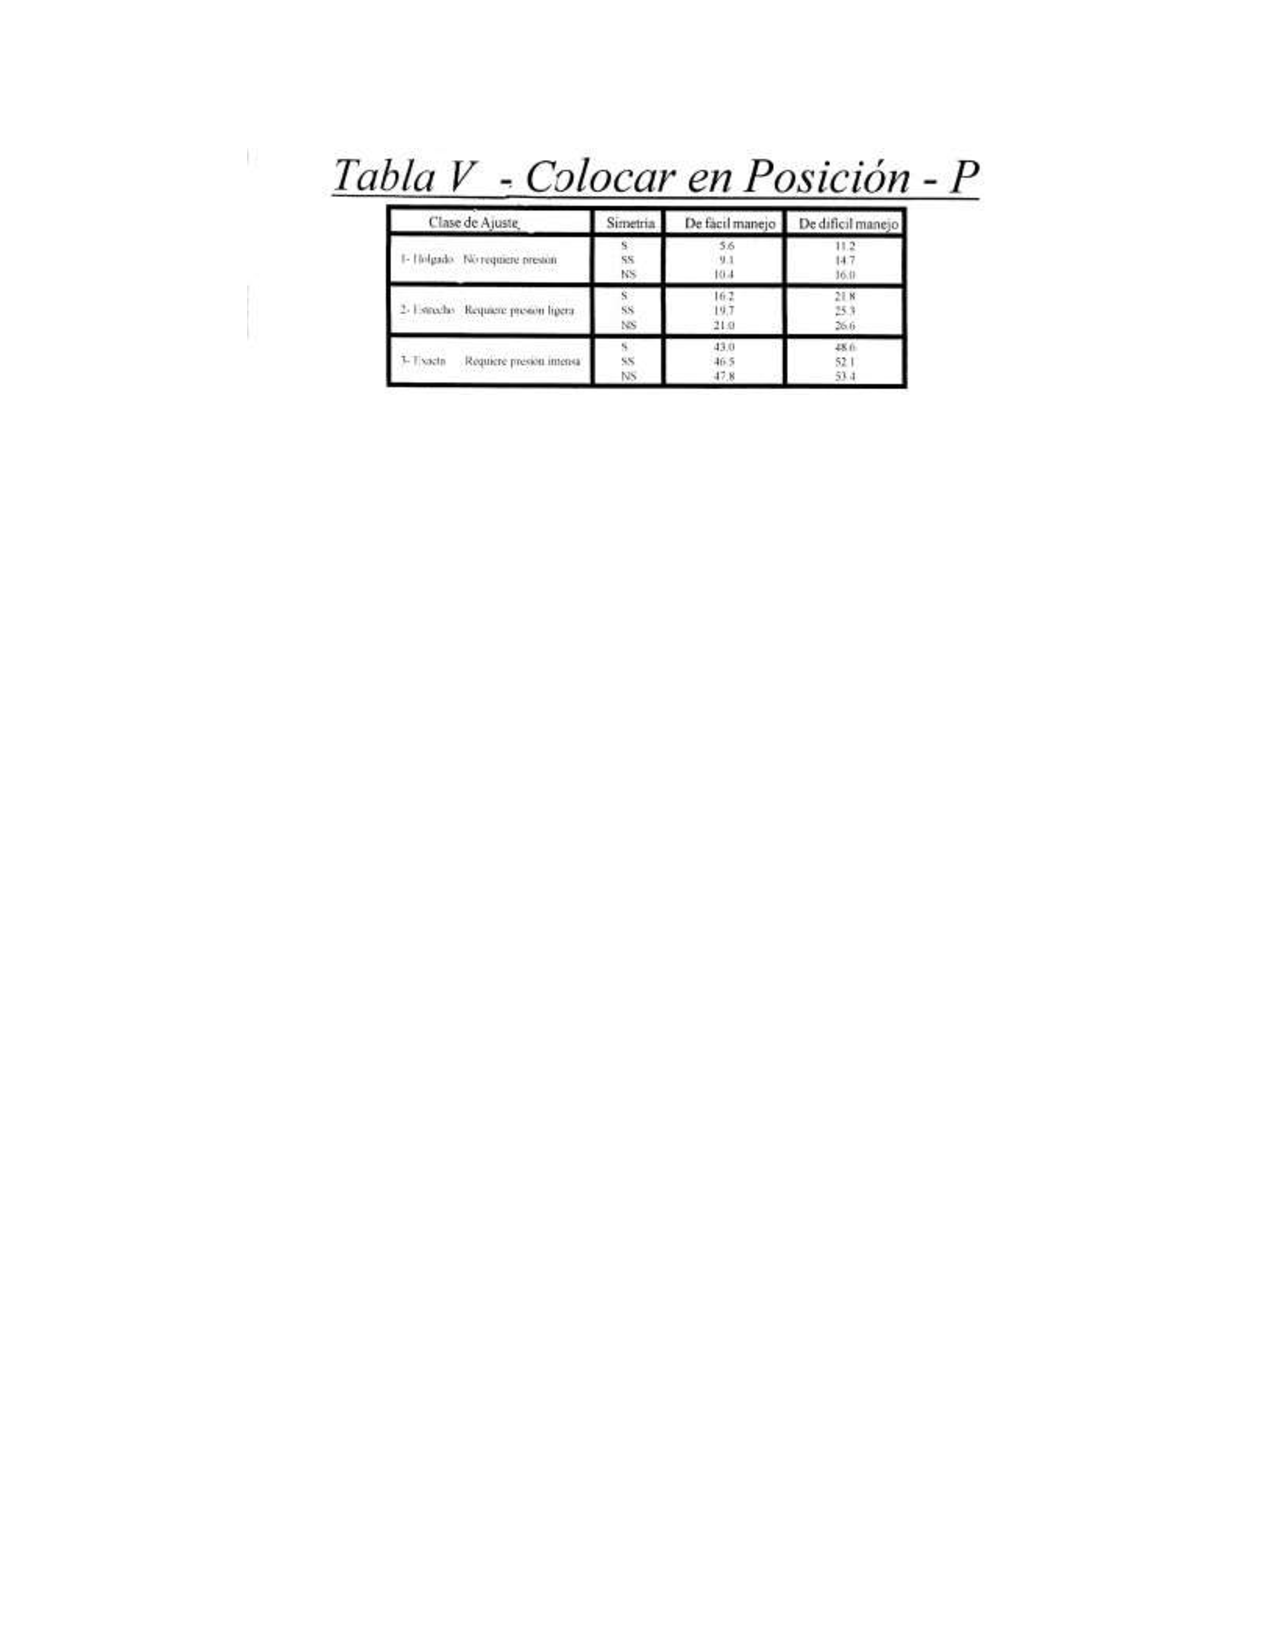
\includegraphics[trim = {42mm 210mm 42mm 24mm},clip,scale=0.6]{19/Img/tablaColocar.pdf}
        \caption{Tabla de tiempos TMU para el movimiento Colocar}
        \label{fig:tablaColocar}
    \end{figure}
\begin{figure}[H]
        \centering
        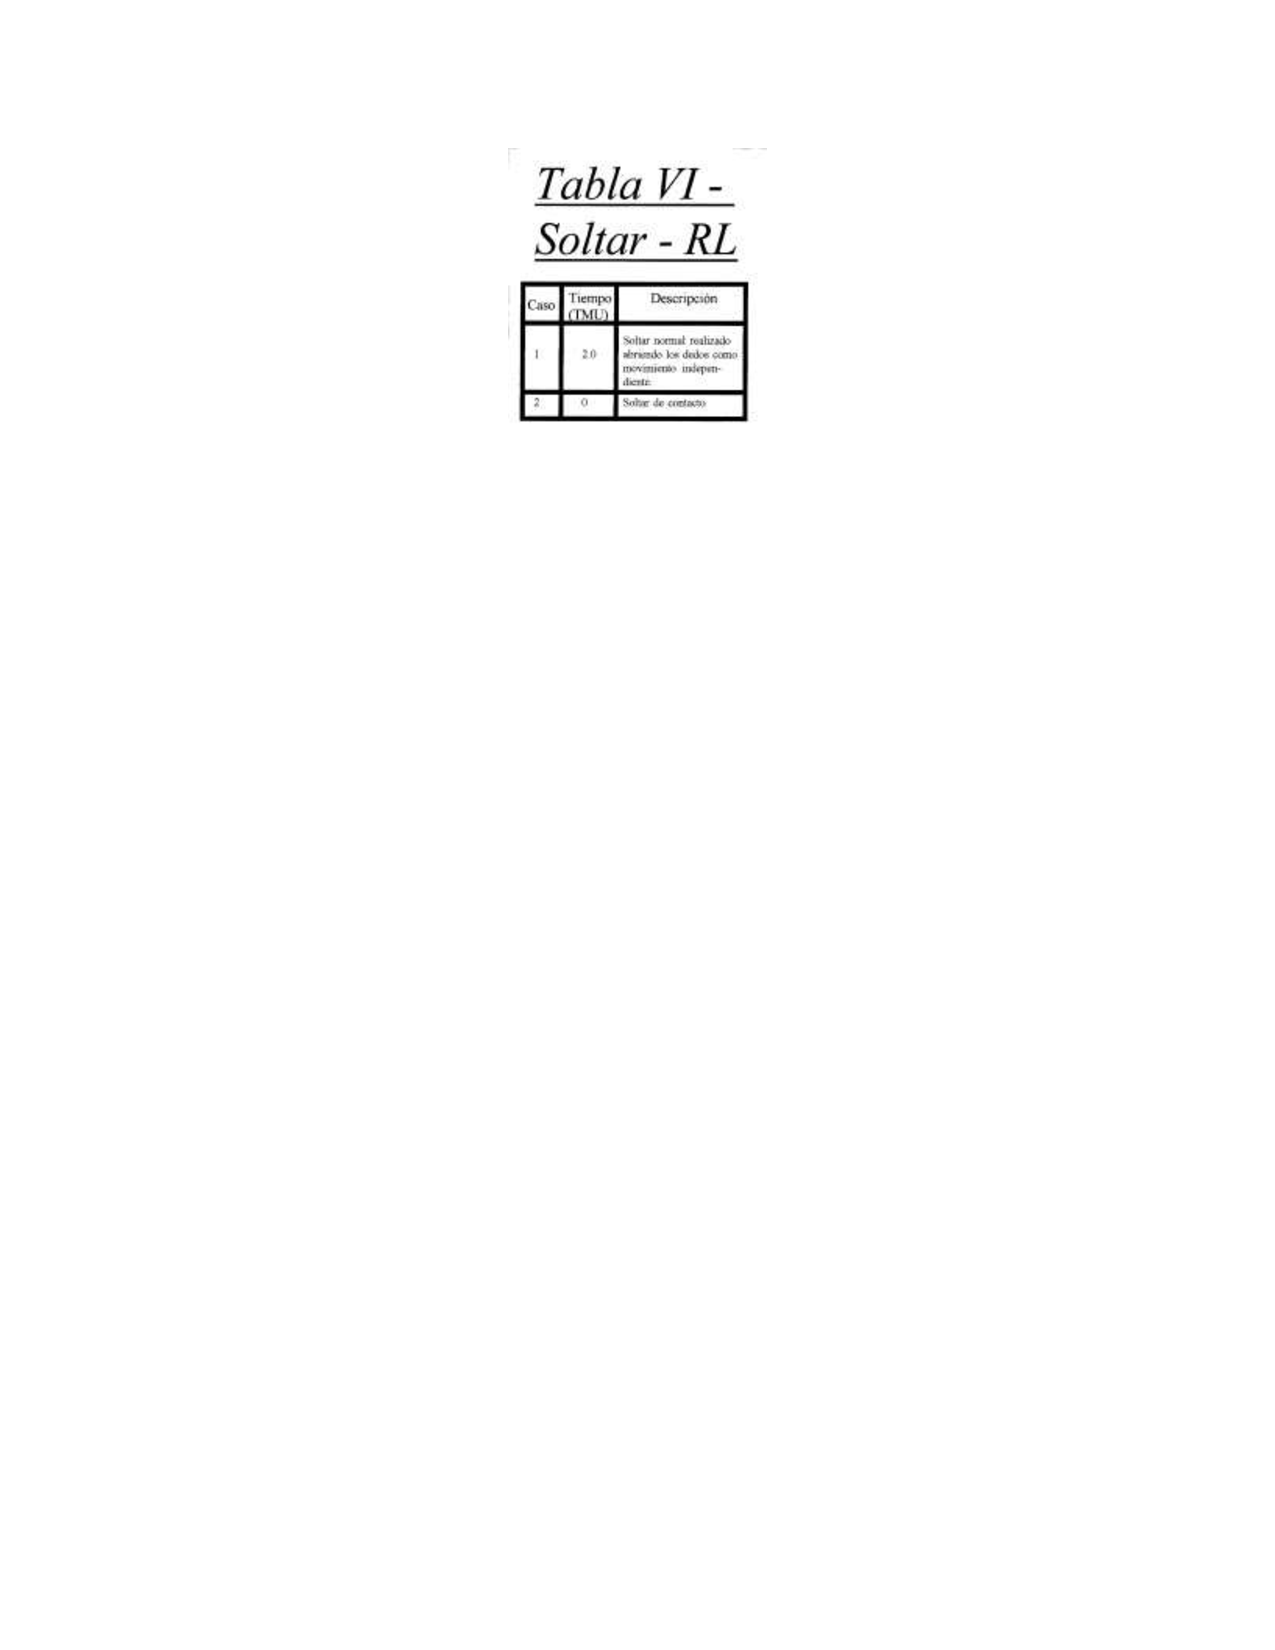
\includegraphics[trim = {42mm 195mm 42mm 24mm},clip,scale=0.6]{19/Img/tablaSoltar.pdf}
        \caption{Tabla de tiempos TMU para el movimiento Soltar}
        \label{fig:tablaSoltar}
    \end{figure}

    Holguras\\
    Para el tiempo obtenido a través de este método es necesario considerar el valor de las holguras otorgadas, ya que no todos los trabajadores pueden hacerlo al 100\% de sus capacidades todo el tiempo, al igual que no puede seguir el ritmo del tiempo "necesario" para realizar la actividad todo el tiempo, por lo que en base a diversos factores a considerar se han generado una tabla de suplementos u "holguras" \ref{fig:tablaHolguras} continuas y variables, las cuales dependiendo de la situación del operario se le otorgará un número el cual representa el porcentaje extra del tiempo ciclo que se le otorgará al trabajador.
    \begin{figure}[H]
        \centering
        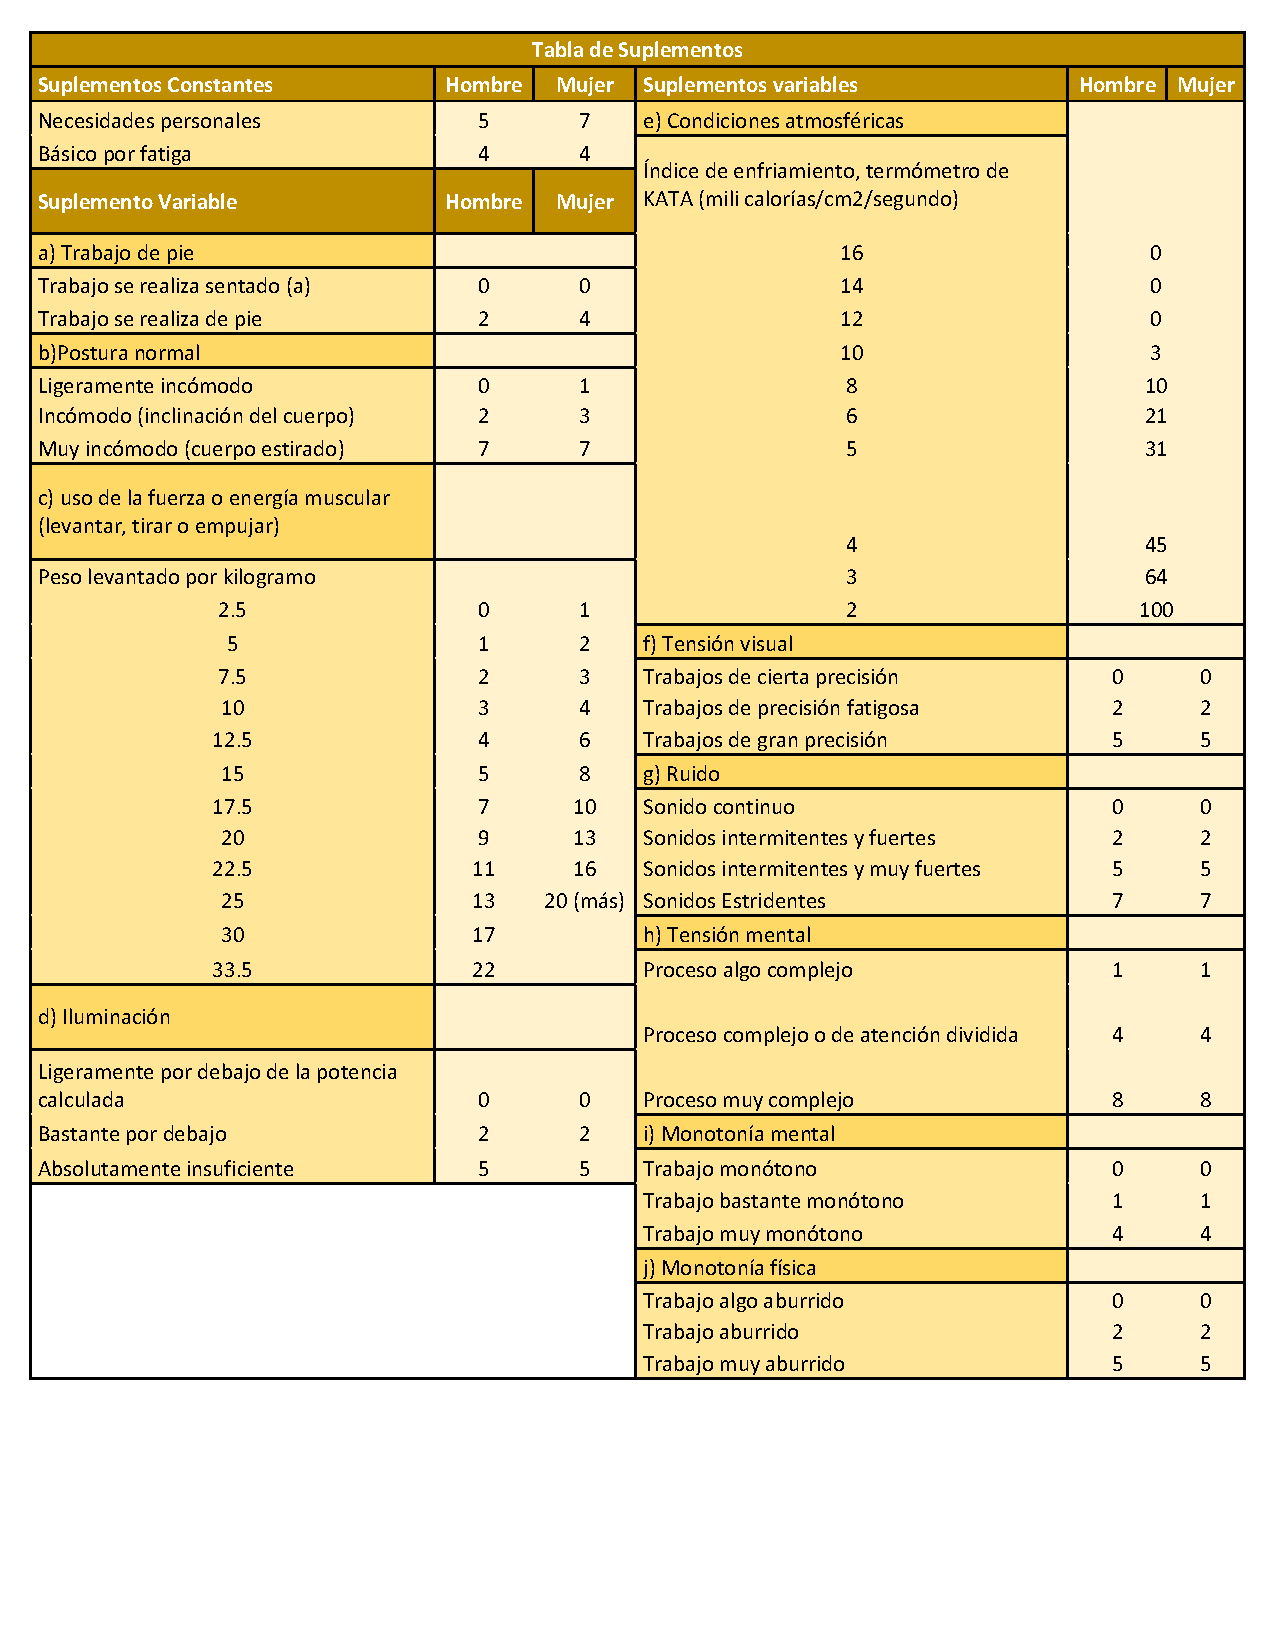
\includegraphics[trim = {1mm 40mm 1mm 1mm},clip,scale=0.4]{19/Img/tablaHolguras.pdf}
        \caption{Tabla de Holguras y suplementos}
        \label{fig:tablaHolguras}
    \end{figure}
\subsubsection{Desarrollo del muestreo del trabajo}
Además del método anterior una forma tal vez incluso más exacta para la obtención de un tiempo estándar al centrarse mas en casos reales es el muestreo del trabajo, el cual en base a las películas de cada ciclo realizado se realiza un análisis de estas para separar el ensamble en cierta cantidad de actividades, las cuales gracias a la película se obtienen sus tiempos. Al ser un grupo limitado de observaciones a analizar se decidió utilizar los valores obtenidos de cada uno de los analistas para usar estos valores como la muestra y de esta manera obtener el tiempo ciclo y estándar para llevar acaba esta actividad.

\subsubsection{Corrección por balanceo de procesos}
También se requerirá de realizar un análisis sobre la parte que llega a afectar o distraer al operario en la estación de trabajo para de esta manera buscar optimizar y mejorar los tiempos de esa parte del ensamblaje.

\subsubsection{Datos estándar continuos y discretos}
Posterior a todo el estudio de tiempos y la obtención de los valores del tiempo estándar se presentaran estos datos de tiempo de manera continua o con diversas pausas que representan una actividad cada una.

\subsection{Diseño de la forma más económica de realizar el trabajo}
     En base a los datos obtenidos con los estudios realizados se planteara una nueva forma de realizar el ensamble, buscando eliminar cualquier tiempo innecesario.
        
\subsection{Normalización de los métodos, materiales, herramientas e instalaciones}
Posterior a esto se buscara estandarizar todos lo necesario para llevar acabo el nuevo método de ensamblaje para de esta manera generar una norma guía para futuros intentos de ensamble.

        Al empezar la metodología establecida para la obtención de los valores de cada ciclo presento los materiales que se utilizaran en el proceso de ensamblaje del circuito, mostrando todo lo necesario en un formato simple de entender y con una imagen de referencia para la comodidad del operador y de los que deseen el replicar el proceso, para posteriormente presentar un manual en que sea presentado también un modelo 3D de la pieza, su costo unitario en el mercado y también la cantidad aproximada de cuantas piezas de cada tipo se requerirán, en conjunto con su manejo.
    
    
        \begin{itemize}
            \item Protoboard: Este es una placa con orificios que tienen conexiones eléctricas entre si en todo el interior de este, estos son usados como base para la generación de circuitos eléctricos, en donde se colocan las resistencias, cables y fuente de corriente o voltaje para comprobar que las funciones del circuito desarrolladas eran las correctas, teniendo lineas tanto de alimentación positiva como negativa para el traspaso de la corriente dentro de esta. Para este circuito se ensamblara y soldara  el ESP-32 al protoboard para alimentar directamente el procesador del ESP-32.\ref{fig:protoboard}.
    
            \begin{figure}[H]
        \centering
        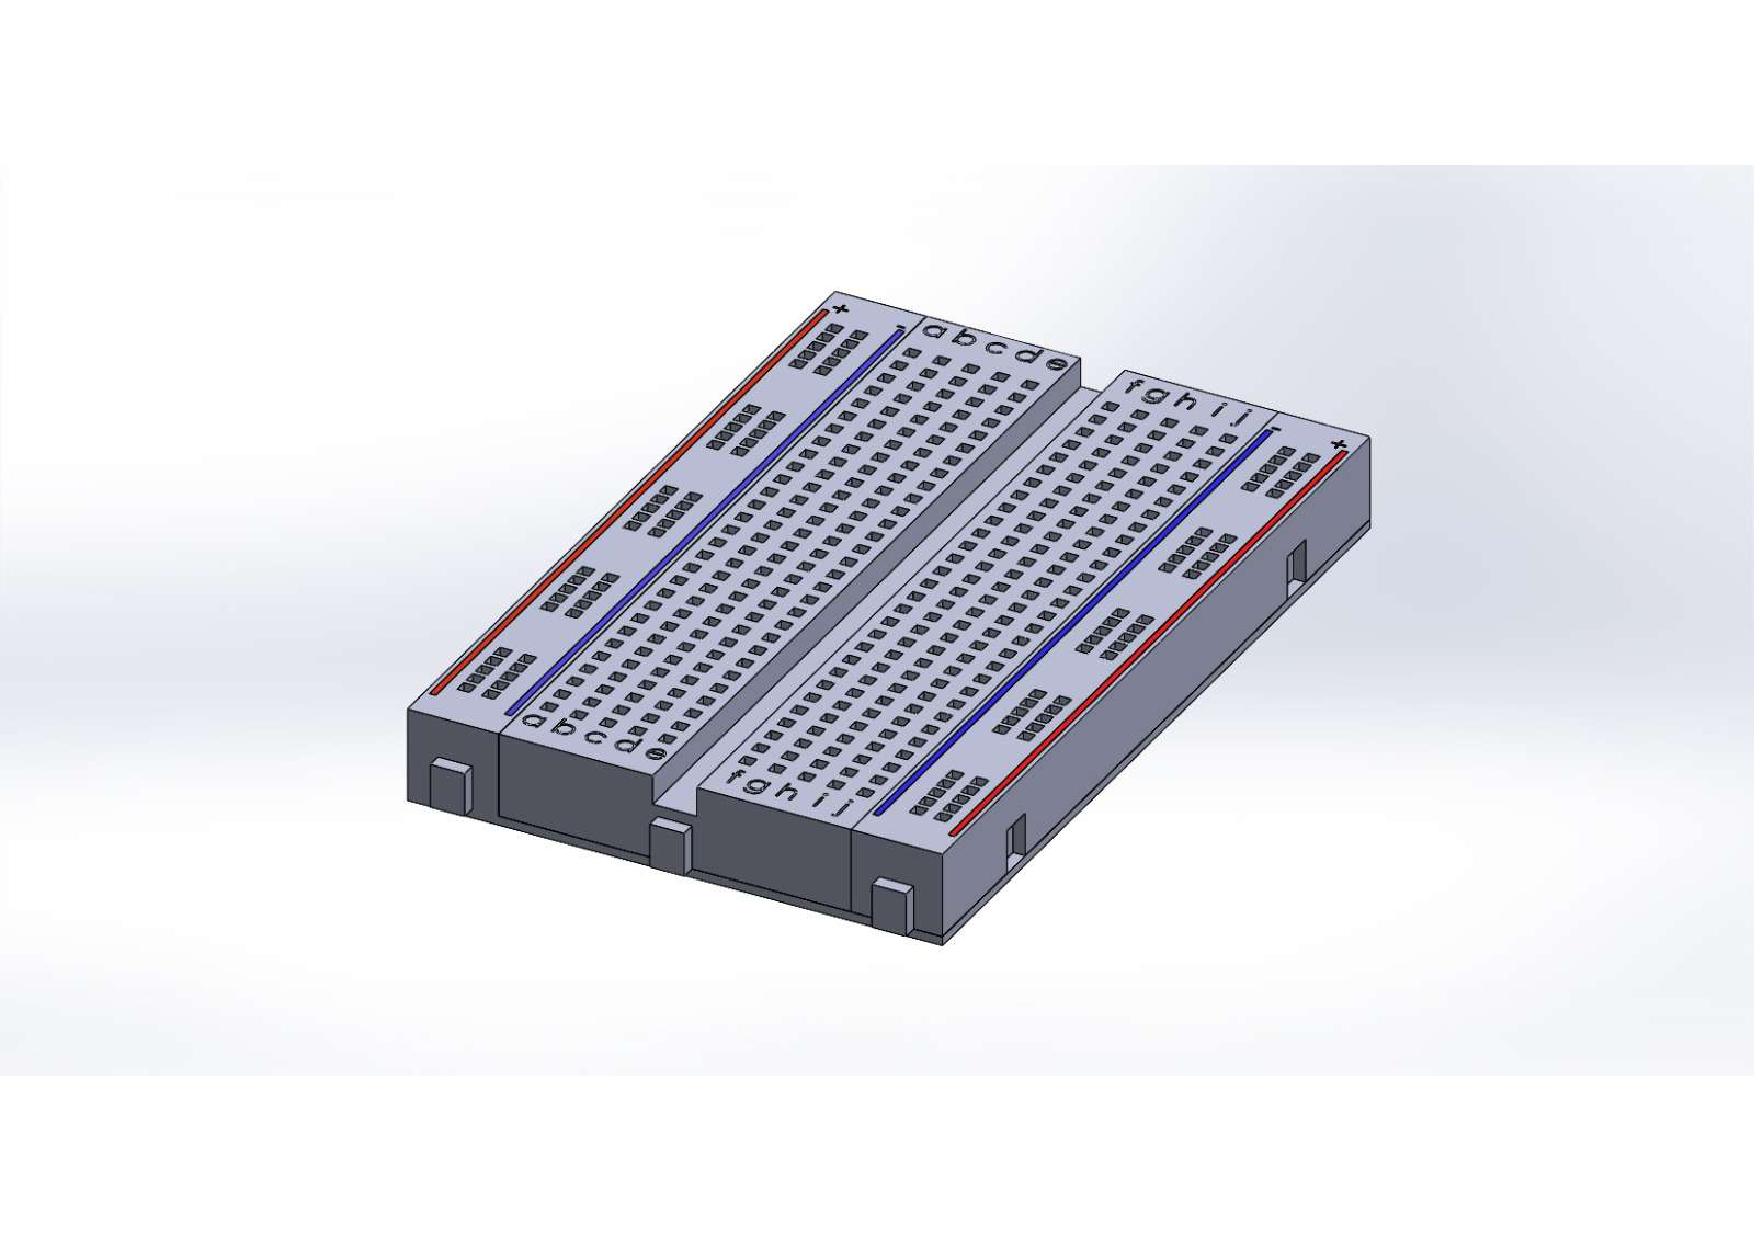
\includegraphics[trim = {65mm 40mm 65mm 40mm},clip,scale=0.5]{19/Img/protoboardFigura.pdf}
        \caption{Imagen del modelo 3D del Protoboard}
        \label{fig:protoboard}
    \end{figure}
    
    \item Resistencia: Pieza de plástico con alambre usada en los circuitos eléctricos como contra para la corriente eléctrica que pasa por ella, disminuyendo o forzando el cambio de dirección de esta corriente, esta se coloca dentro de los orificios del Protoboard para facilitar el flujo deseado de la corriente.\ref{fig:resistencia}.
    
            \begin{figure}[H]
        \centering
        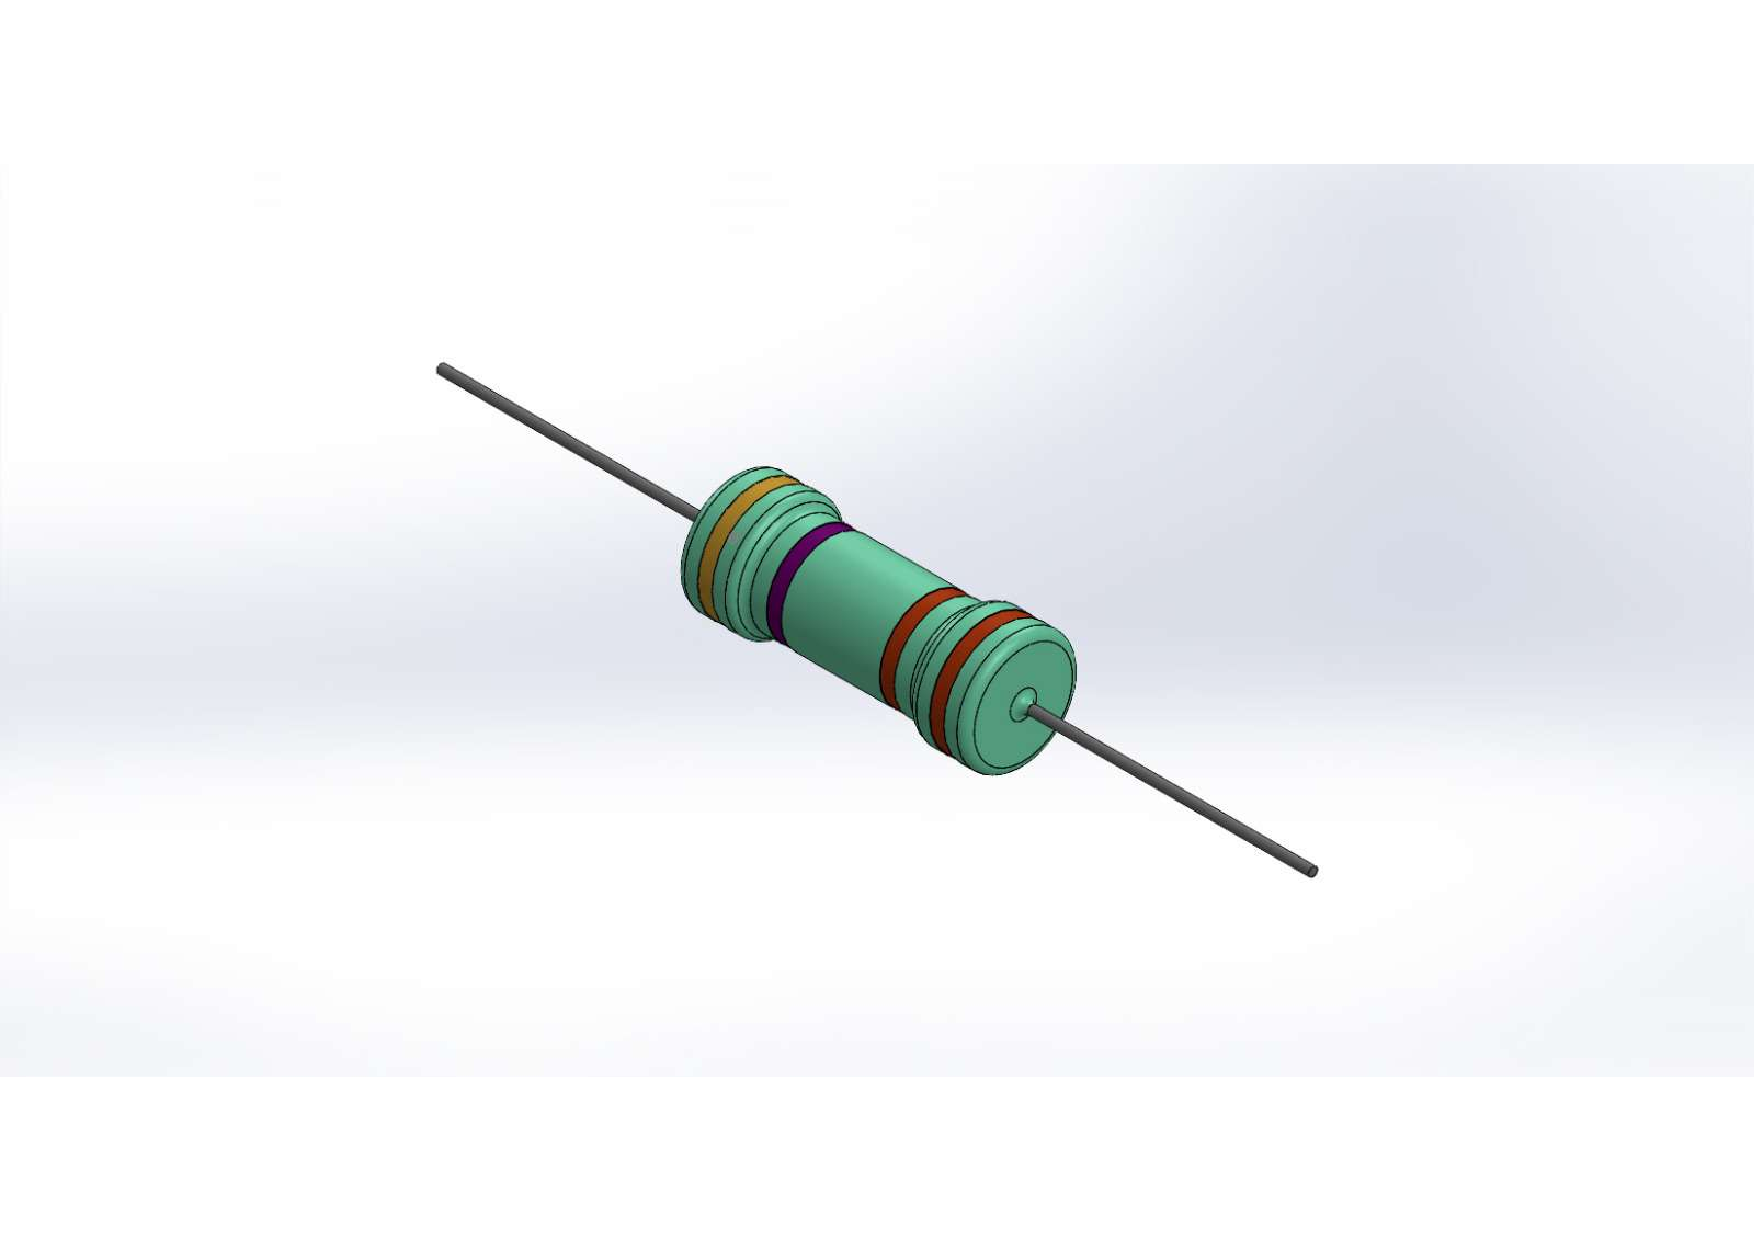
\includegraphics[trim = {65mm 40mm 80mm 60mm},clip,scale=0.5]{19/Img/resistenciaFigura.pdf}
        \caption{Imagen del modelo 3D de la resistencia}
        \label{fig:resistencia}
    \end{figure}
    
    \item Cable MM: Tipo de cable usado en la fabricación de circuitos eléctricos, este posee una varilla de metal por ambos lados lo cual permite el conectar dos elementos del tablero del Protoboard directamente.\ref{fig:cableMM}.
    
            \begin{figure}[H]
        \centering
        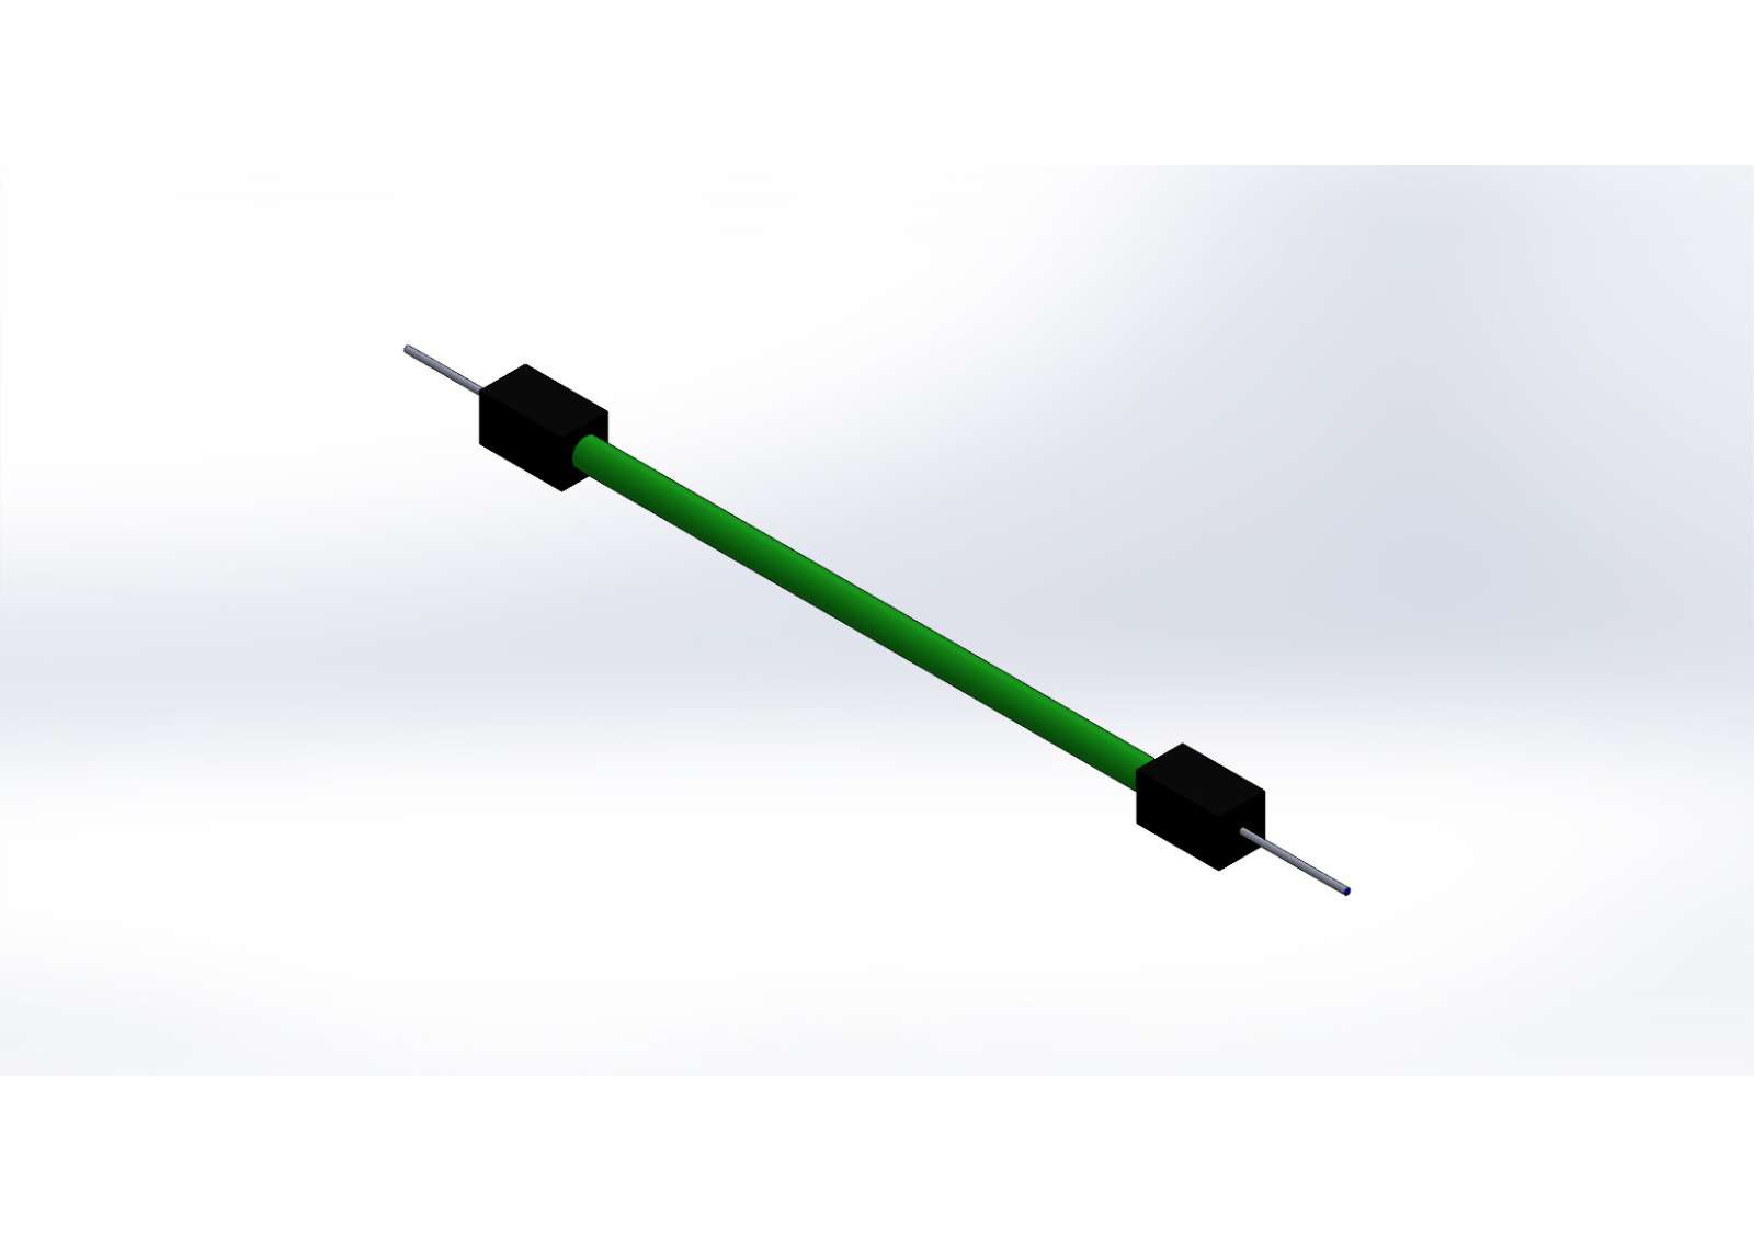
\includegraphics[trim = {70mm 60mm 60mm 50mm},clip,scale=0.5]{19/Img/cableMMFigura.pdf}
        \caption{Imagen del modelo 3D del cable MM}
        \label{fig:cableMM}
    \end{figure}
    
    \item Cable MH: Tipo de cable usado en la fabricación de circuitos eléctricos, este posee una varilla de metal solo por un lado del cable por lo cual este es usada comúnmente como extensión para que otro cable llegue a conectarse con otro que se encuentre a mayor distancia.\ref{fig:cableMH}.
    
            \begin{figure}[H]
        \centering
        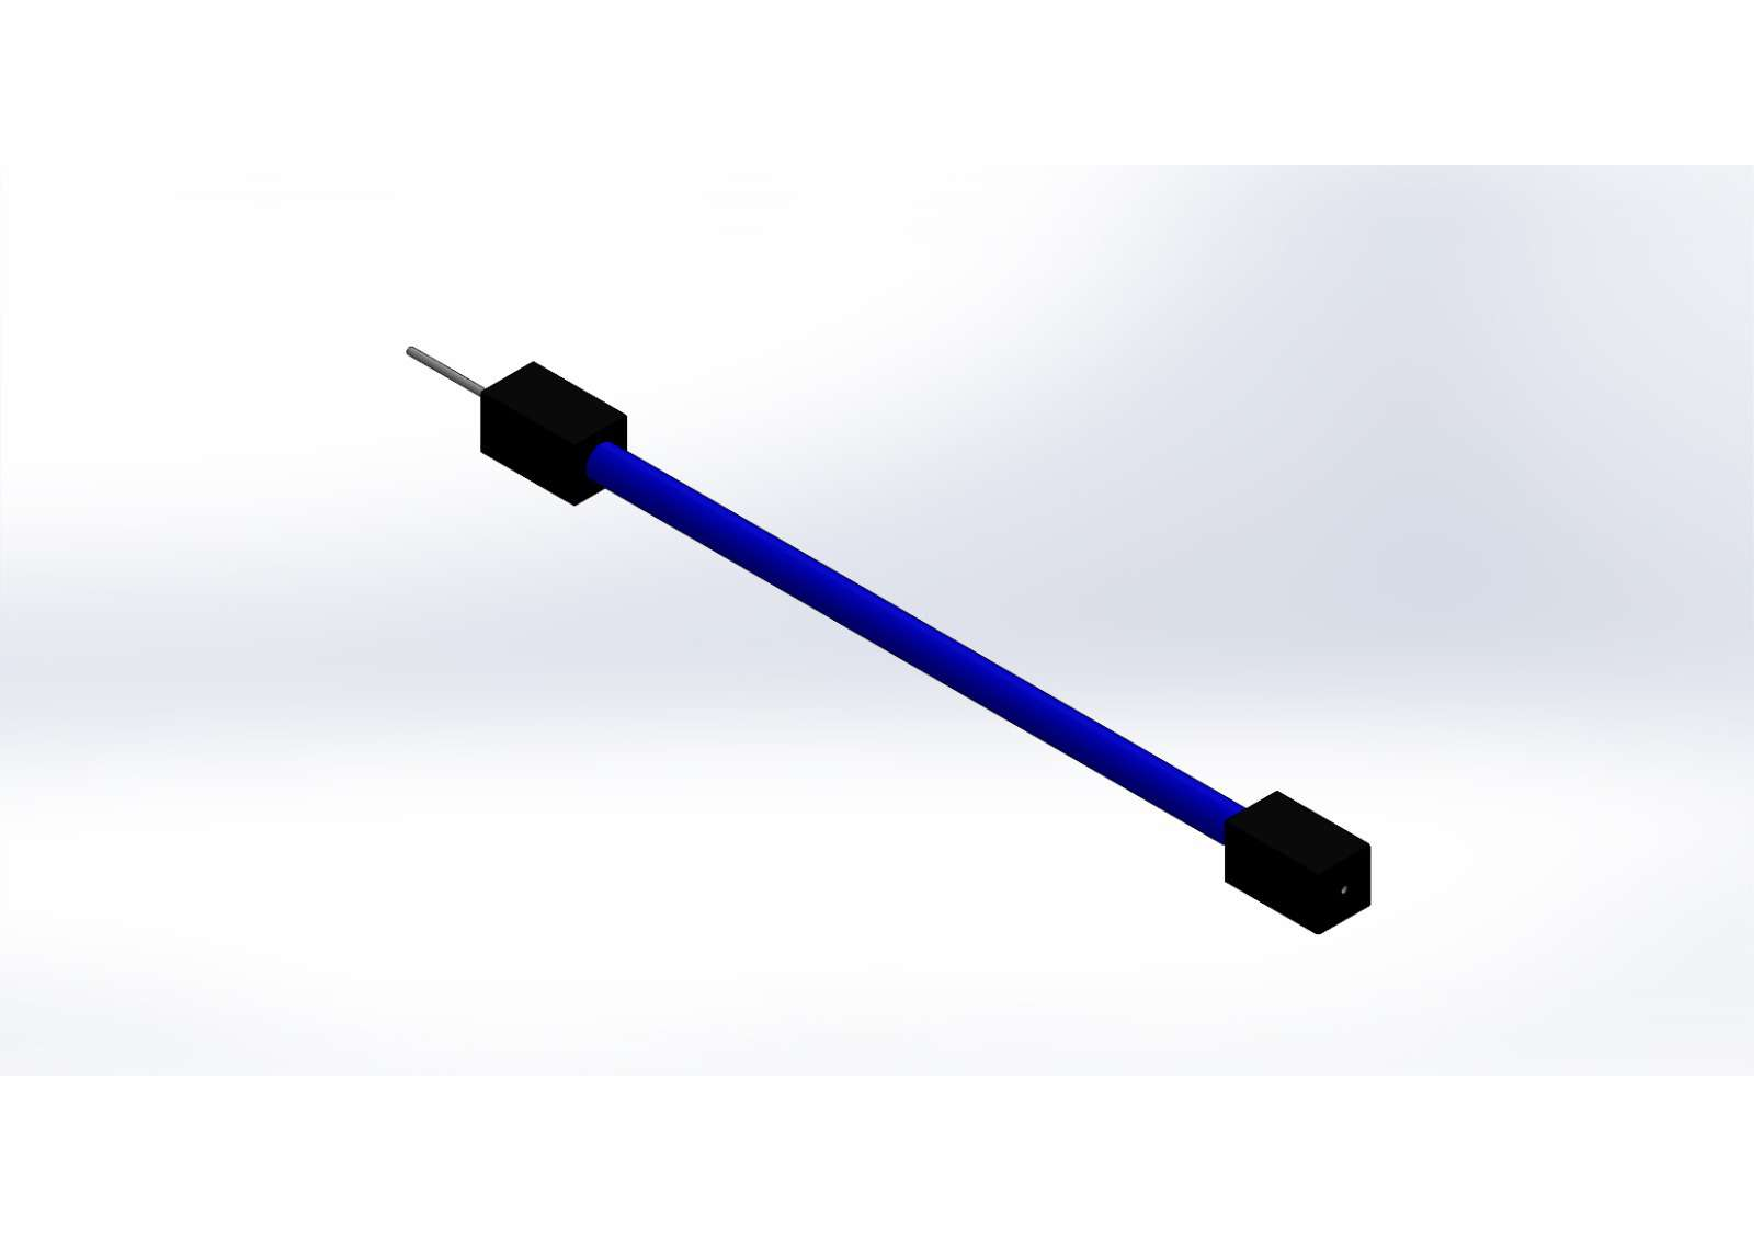
\includegraphics[trim = {65mm 30mm 60mm 40mm},clip,scale=0.5]{19/Img/cableMHFigura.pdf}
        \caption{Imagen del modelo 3D del cable MH}
        \label{fig:cableMH}
    \end{figure}
    
    \item Potenciómetro: Este posee el mismo funcionamiento que una resistencia, con la diferencia de que este puede variar, pudiendo modificar el valor de esta para colocarle el valor deseado, para mantener controlada la corriente total del circuito.\ref{fig:Potenciómetro}.
    
            \begin{figure}[H]
        \centering
        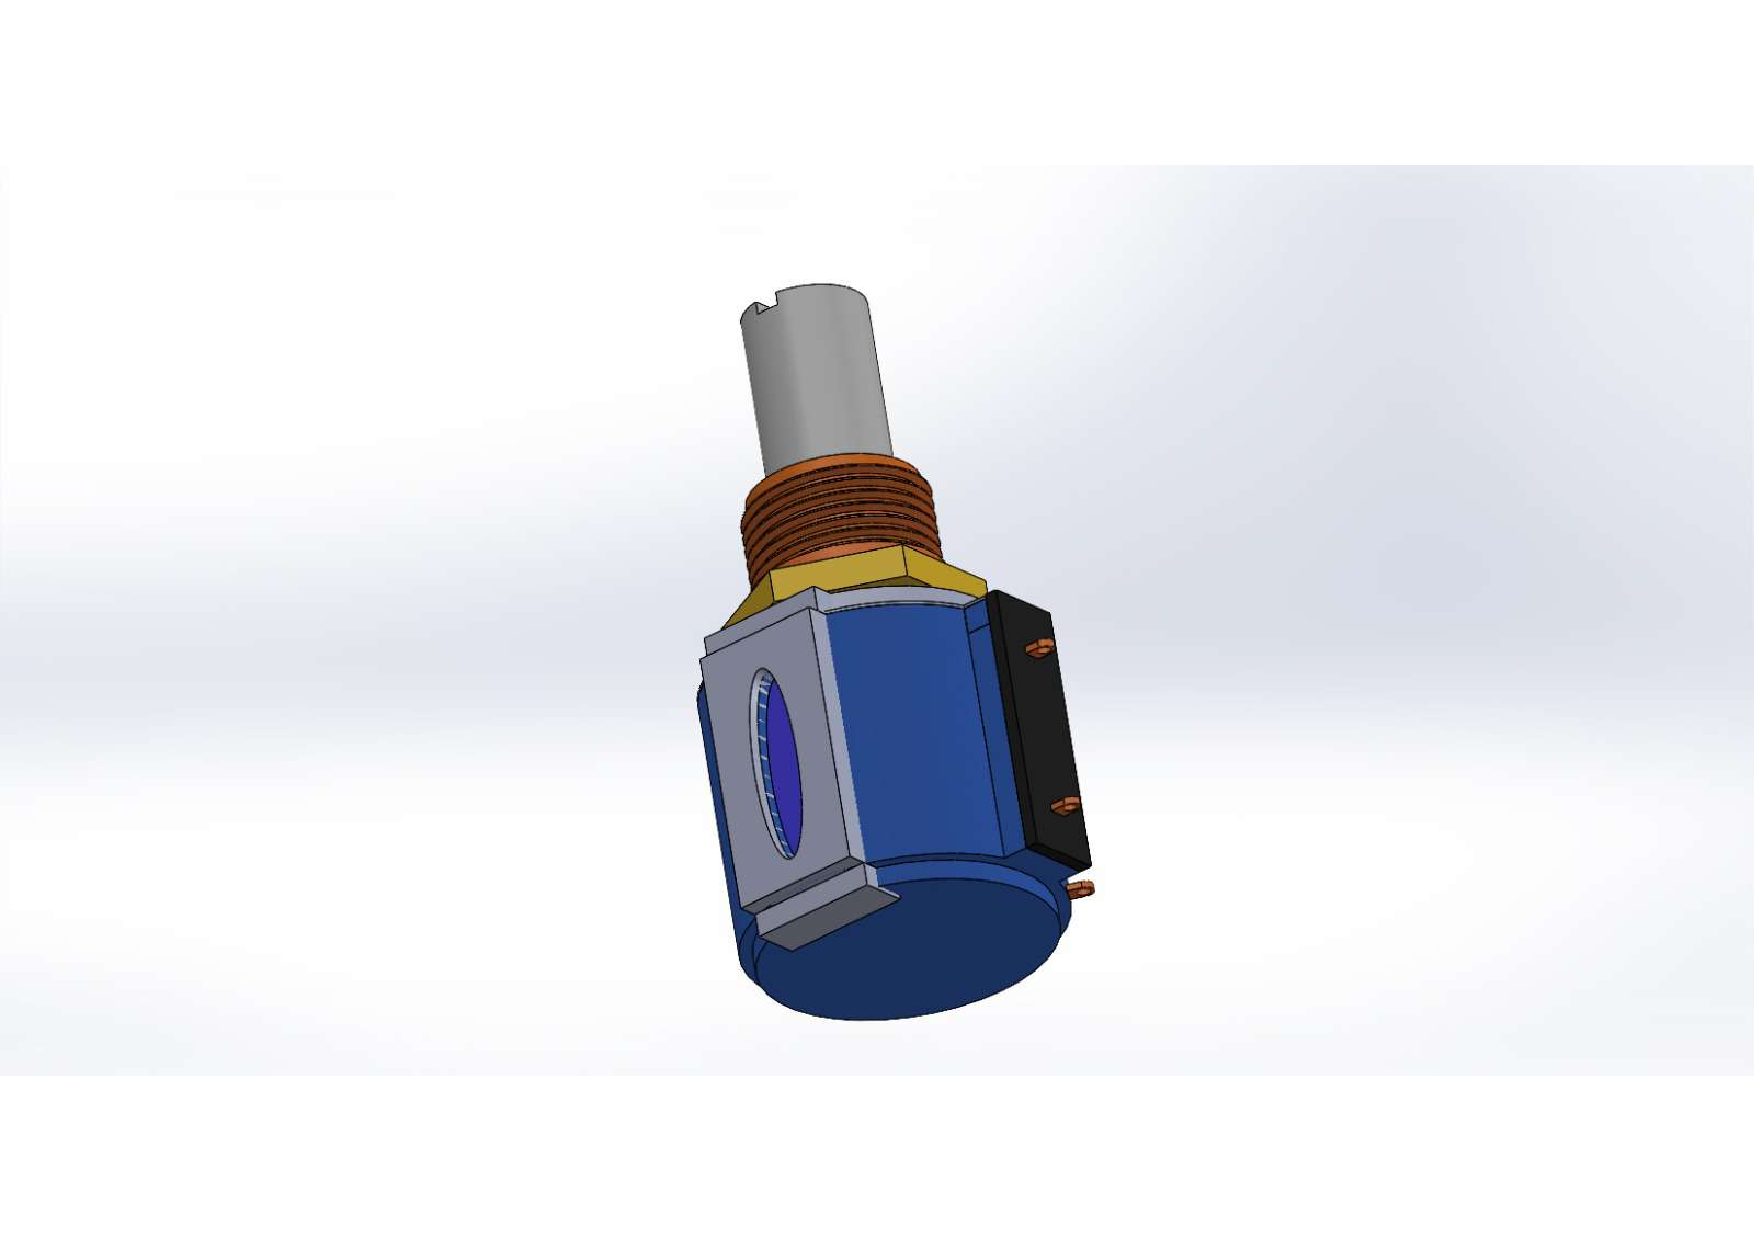
\includegraphics[trim = {65mm 30mm 60mm 40mm},clip,scale=0.5]{19/Img/potenciometroFigura.pdf}
        \caption{Imagen del modelo 3D del Potenciómetro}
        \label{fig:Potenciómetro}
    \end{figure}
        
    \item LCD: Pequeño dispositivo que posee una pantalla de cristal líquido, el cual es usado principalmente en los circuitos eléctricos para comprobar el funcionamiento de todas las piezas, mostrando mensajes que se programan con anterioridad dentro del circuito.\ref{fig:LCD}.
    
            \begin{figure}[H]
        \centering
        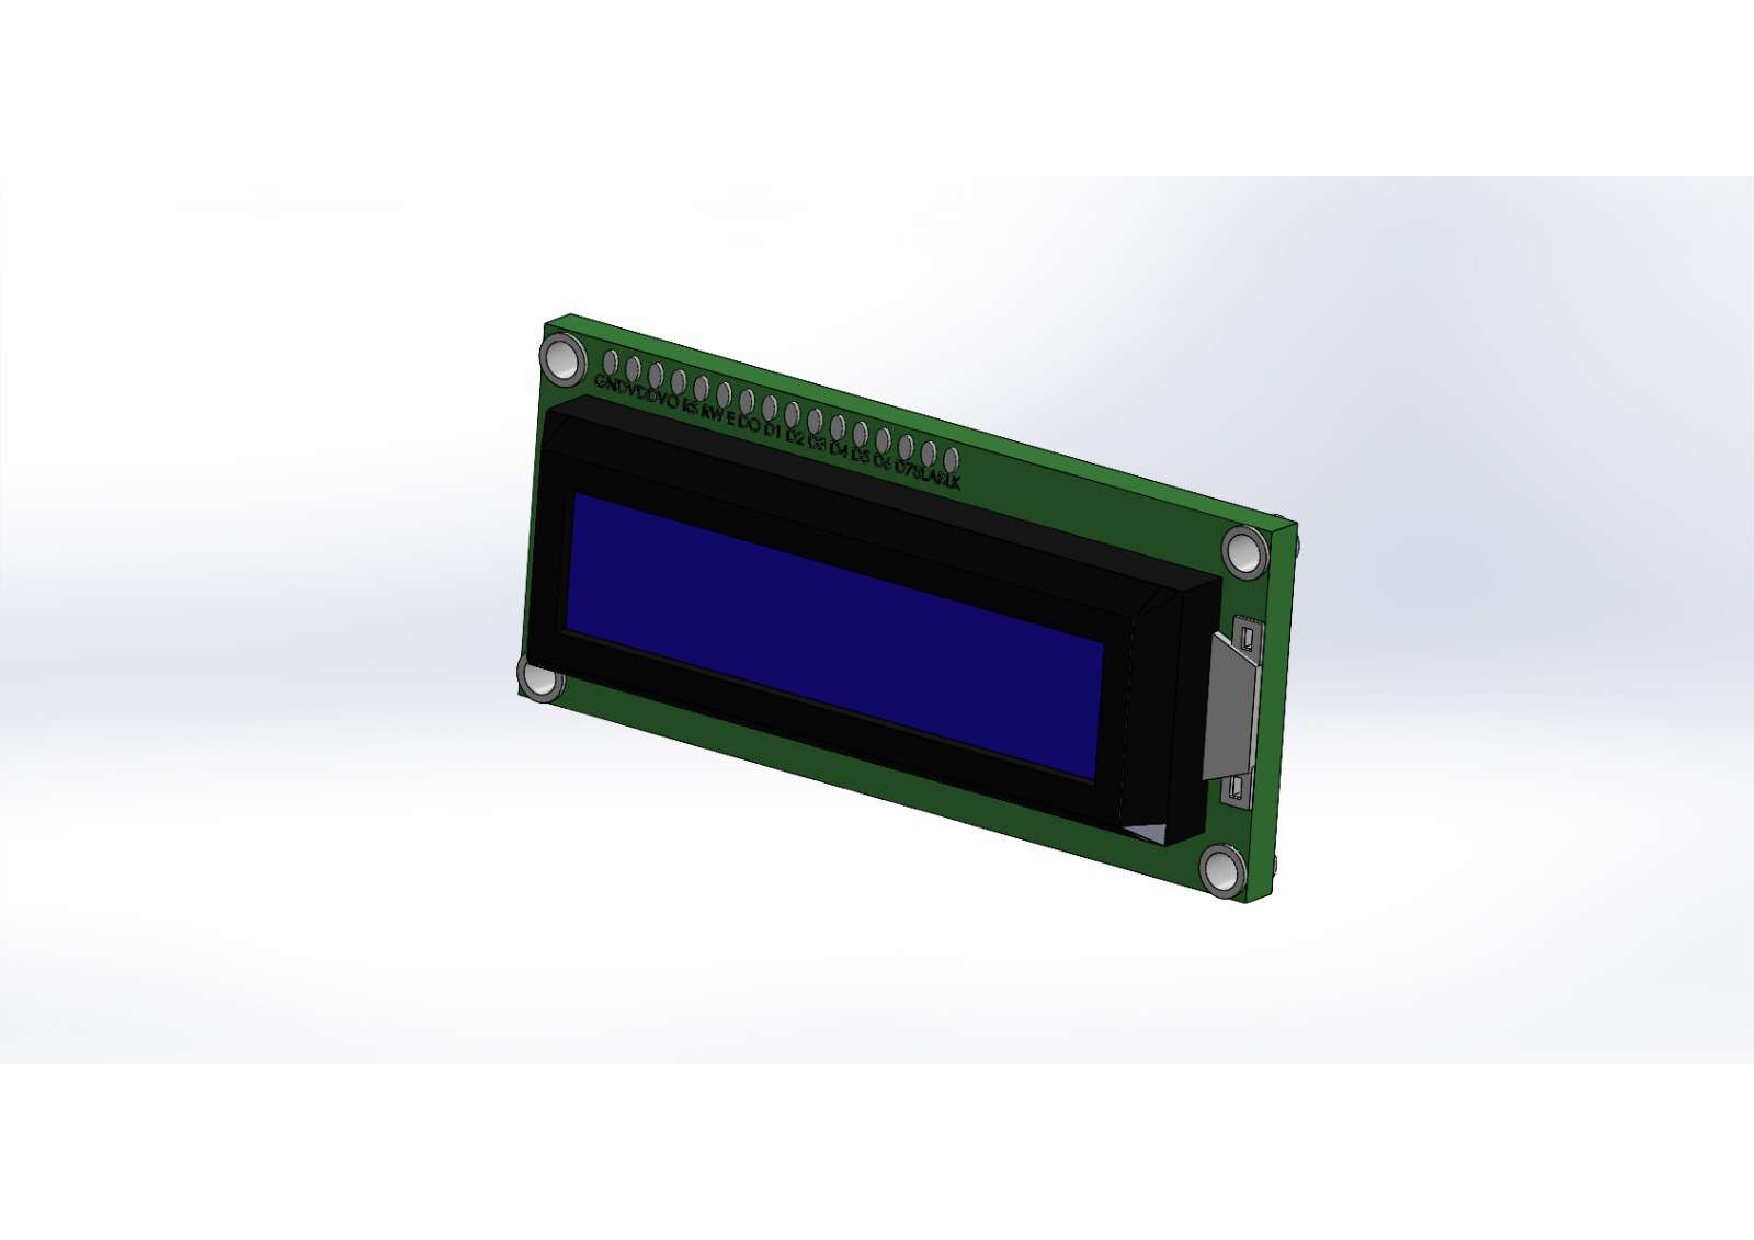
\includegraphics[trim = {65mm 60mm 60mm 50mm},clip,scale=0.5]{19/Img/icdFigura.pdf}
        \caption{Imagen del modelo 3D del LCD}
        \label{fig:LCD}
    \end{figure}
    
    \item Extensión: Objeto usado para expandir el cable conectado al circuito para que este pueda llegar a la fuente de energía.\ref{fig:Extension}.
    
            \begin{figure}[H]
        \centering
        \includegraphics[trim = {65mm 40mm 60mm 40mm},clip,scale=0.5]{19/Img/extensiónFigura.pdf}
        \caption{Imagen del modelo 3D de la Extensión}
        \label{fig:Extension}
    \end{figure}
    
    \item Cable USB: Cable usado para darle una fuente de energía directa al circuito eléctrico, este posee dos conexiones iguales saliendo de ambos lados del cable.\ref{fig:CableUSB}.
    
            \begin{figure}[H]
        \centering
        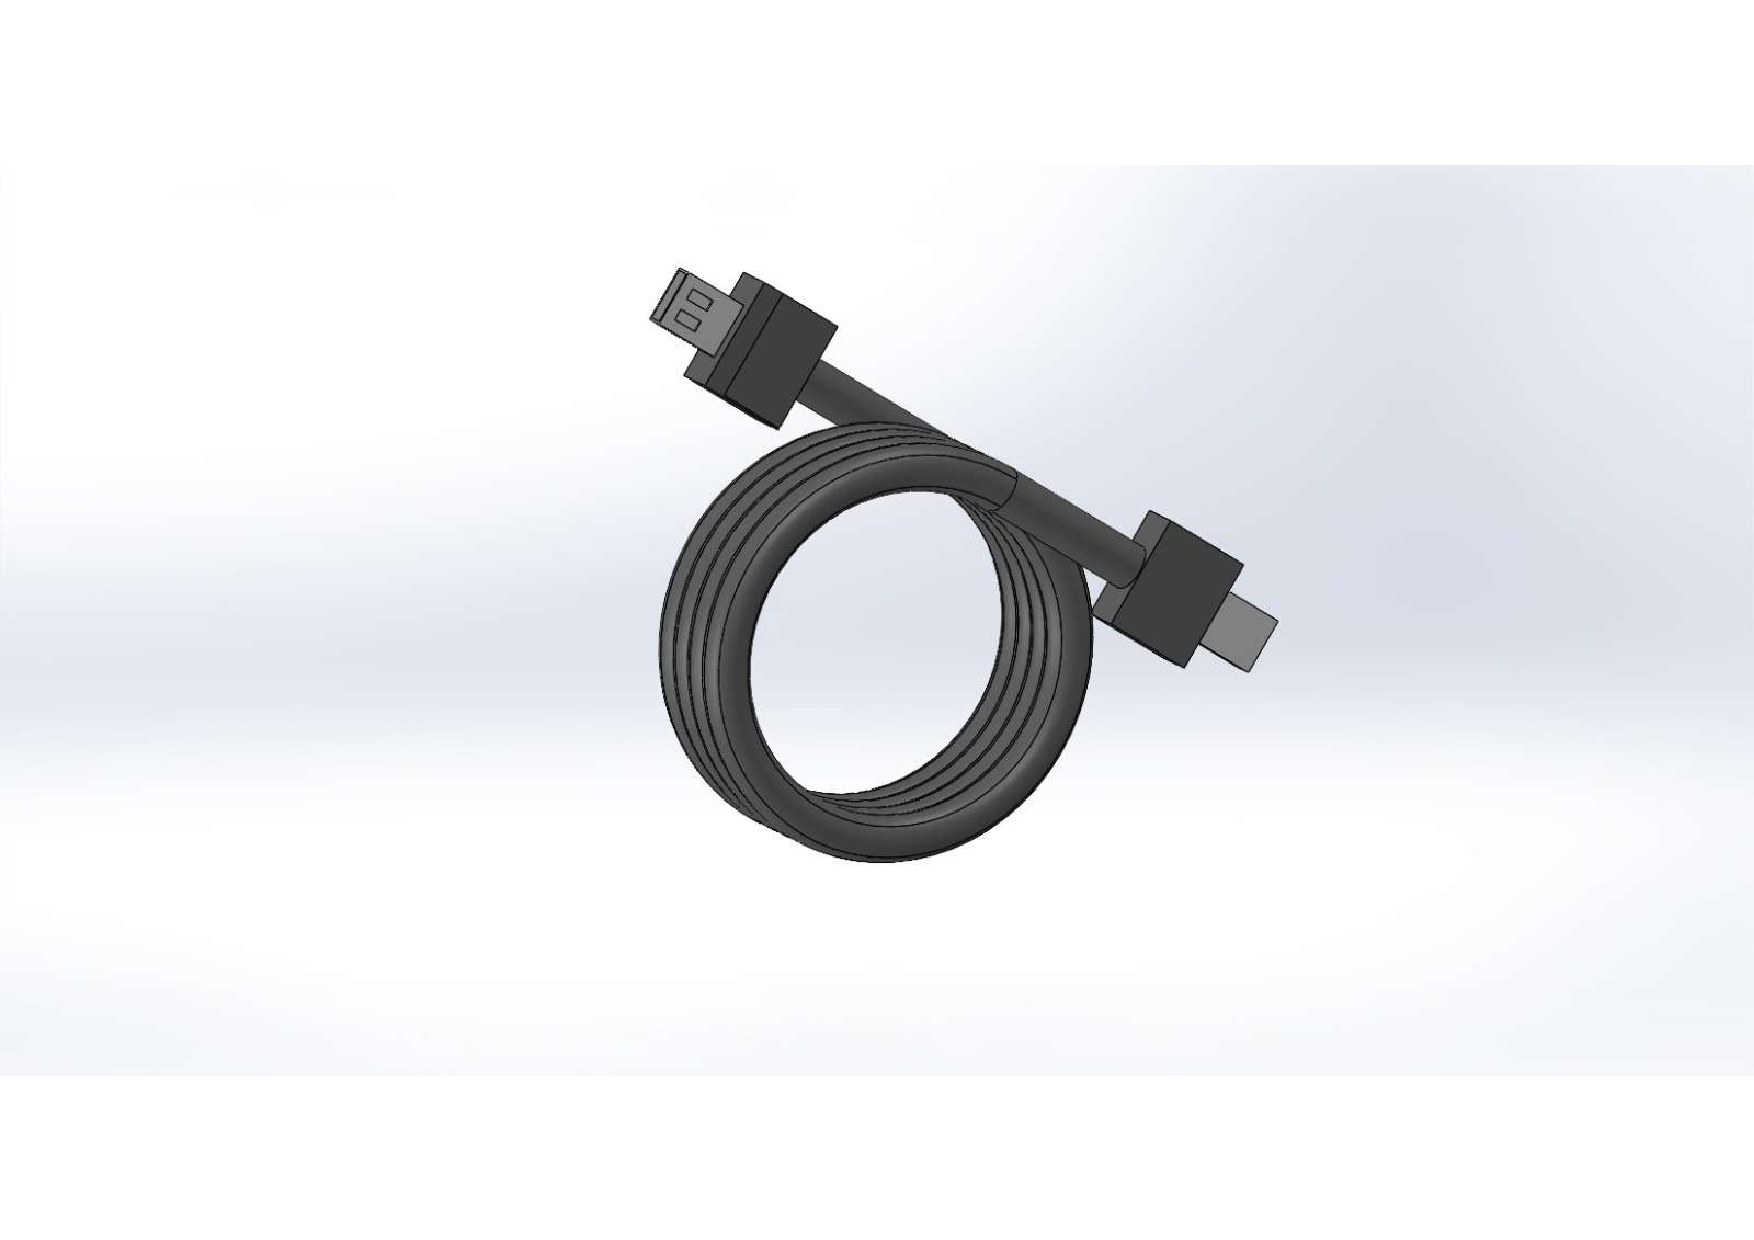
\includegraphics[trim = {65mm 40mm 60mm 40mm},clip,scale=0.5]{19/Img/cableUSBFigura.pdf}
        \caption{Imagen del modelo 3D del cable USB}
        \label{fig:CableUSB}
    \end{figure}
    
    \item ESP-32: Este chip es un microcontrolador soldado directamente al Protoboard, el cual permite poseer tanto un receptor como un emisor de señal saliente del Protoboard.\ref{fig:ESP-32}.
    
            \begin{figure}[H]
        \centering
        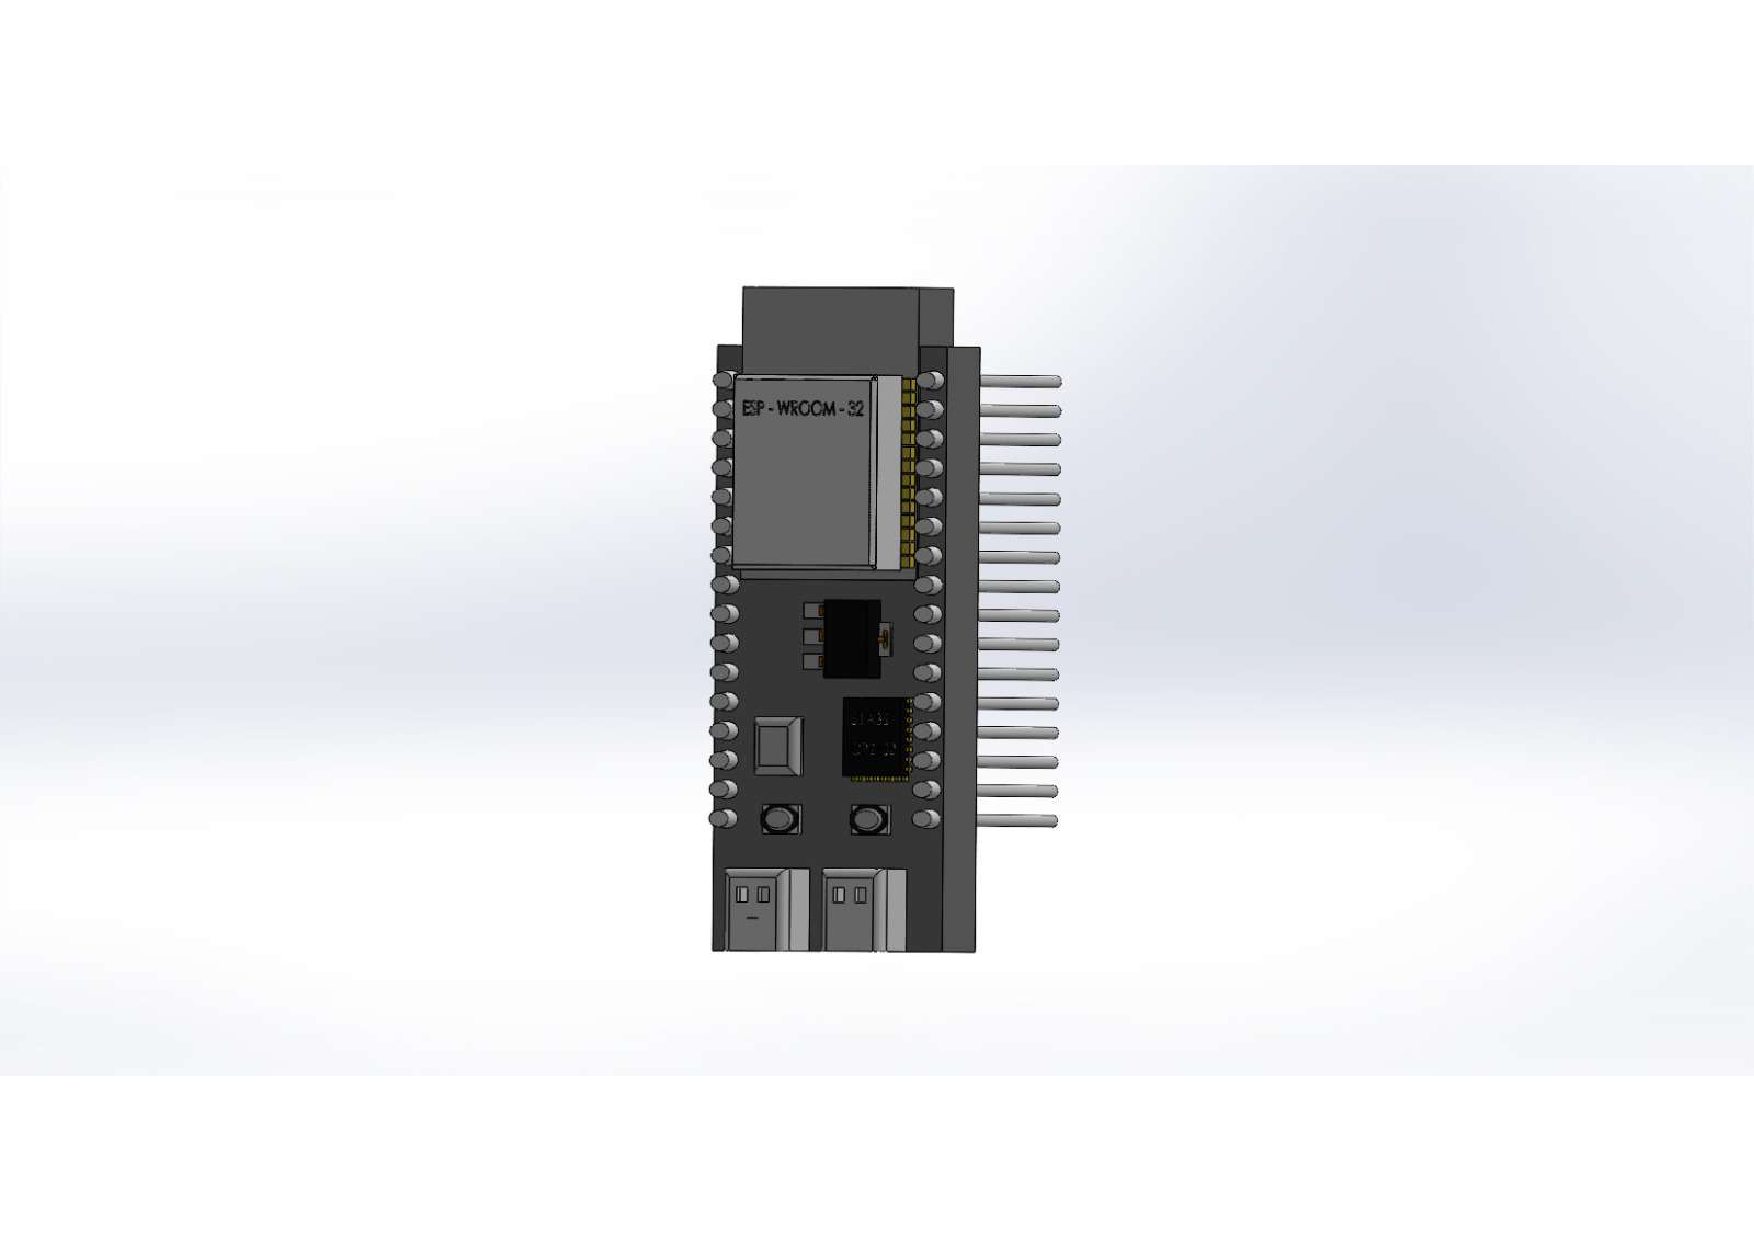
\includegraphics[trim = {65mm 35mm 60mm 40mm},clip,scale=0.5]{19/Img/esp32Figura.pdf}
        \caption{Imagen del modelo 3D del ESP-32}
        \label{fig:ESP-32}
    \end{figure}
    
    \item Módulo I2C Interfaz: Este es un modulo de interfaz que permite facilitar el manejo y utilización de las pantallas, siendo soldada en la parte posterior de la LCD para su uso en el circuito.\ref{fig:modulo}.
    
            \begin{figure}[H]
        \centering
        \includegraphics[trim = {65mm 35mm 60mm 40mm},clip,scale=0.5]{19/Img/móduloI2CInterfazFigura.pdf}
        \caption{Imagen del modelo 3D del Módulo I2C Interfaz}
        \label{fig:modulo}
    \end{figure}
        \end{itemize}
    
    
    A continuación presentare una lista de dibujos de las piezas a utilizar con el propósito de ofrecer las medidas base que se emplearan de cada material a la hora de realizar el ensamble del circuito presentado en este proceso:
                \begin{figure}[H]
        \centering
        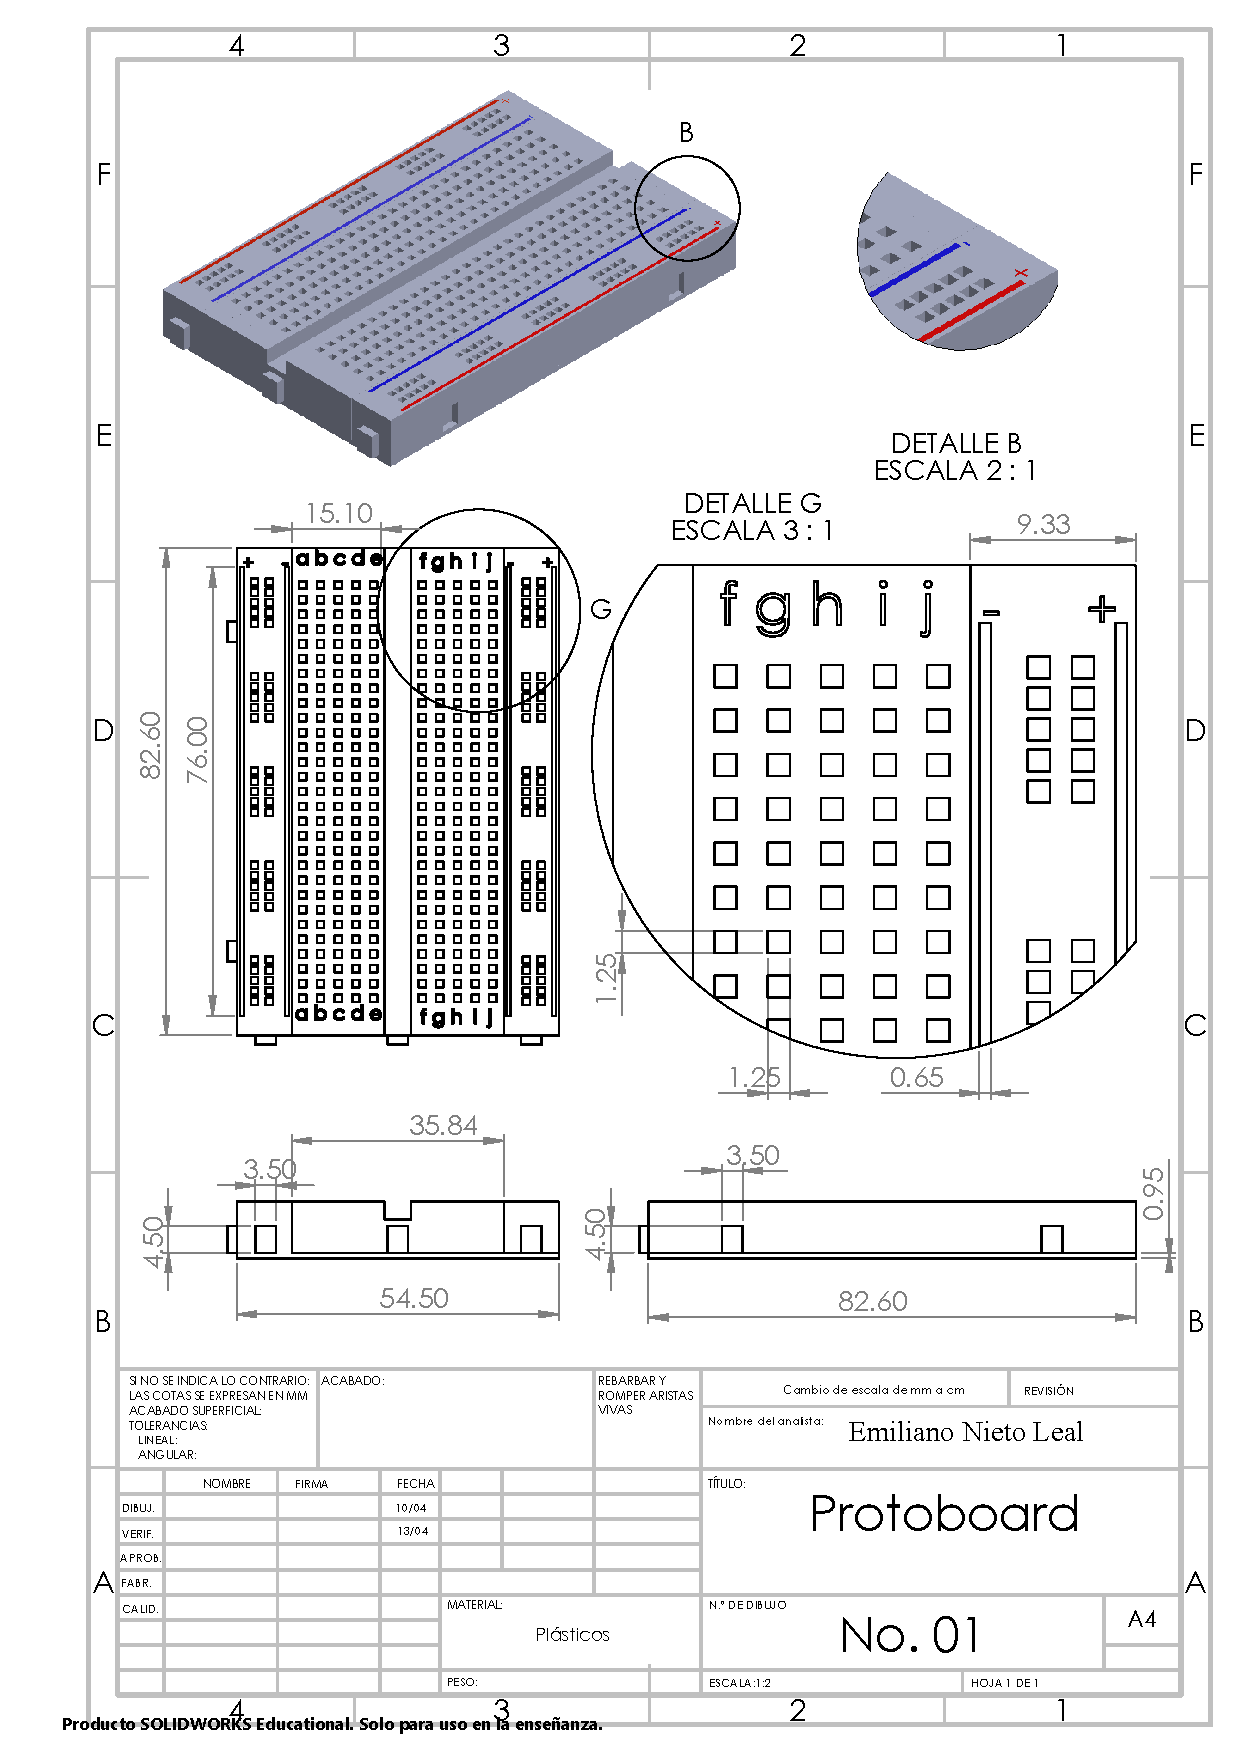
\includegraphics[trim = {1mm 1mm 1mm 1mm},clip,scale=0.3]{19/Img/protoboardDibujo.pdf}
        \caption{Dibujo Protoboard}
        \label{fig:Dibujo Protoboard}
    \end{figure}
        
    
    \newpage
                \begin{figure}[H]
        \centering
        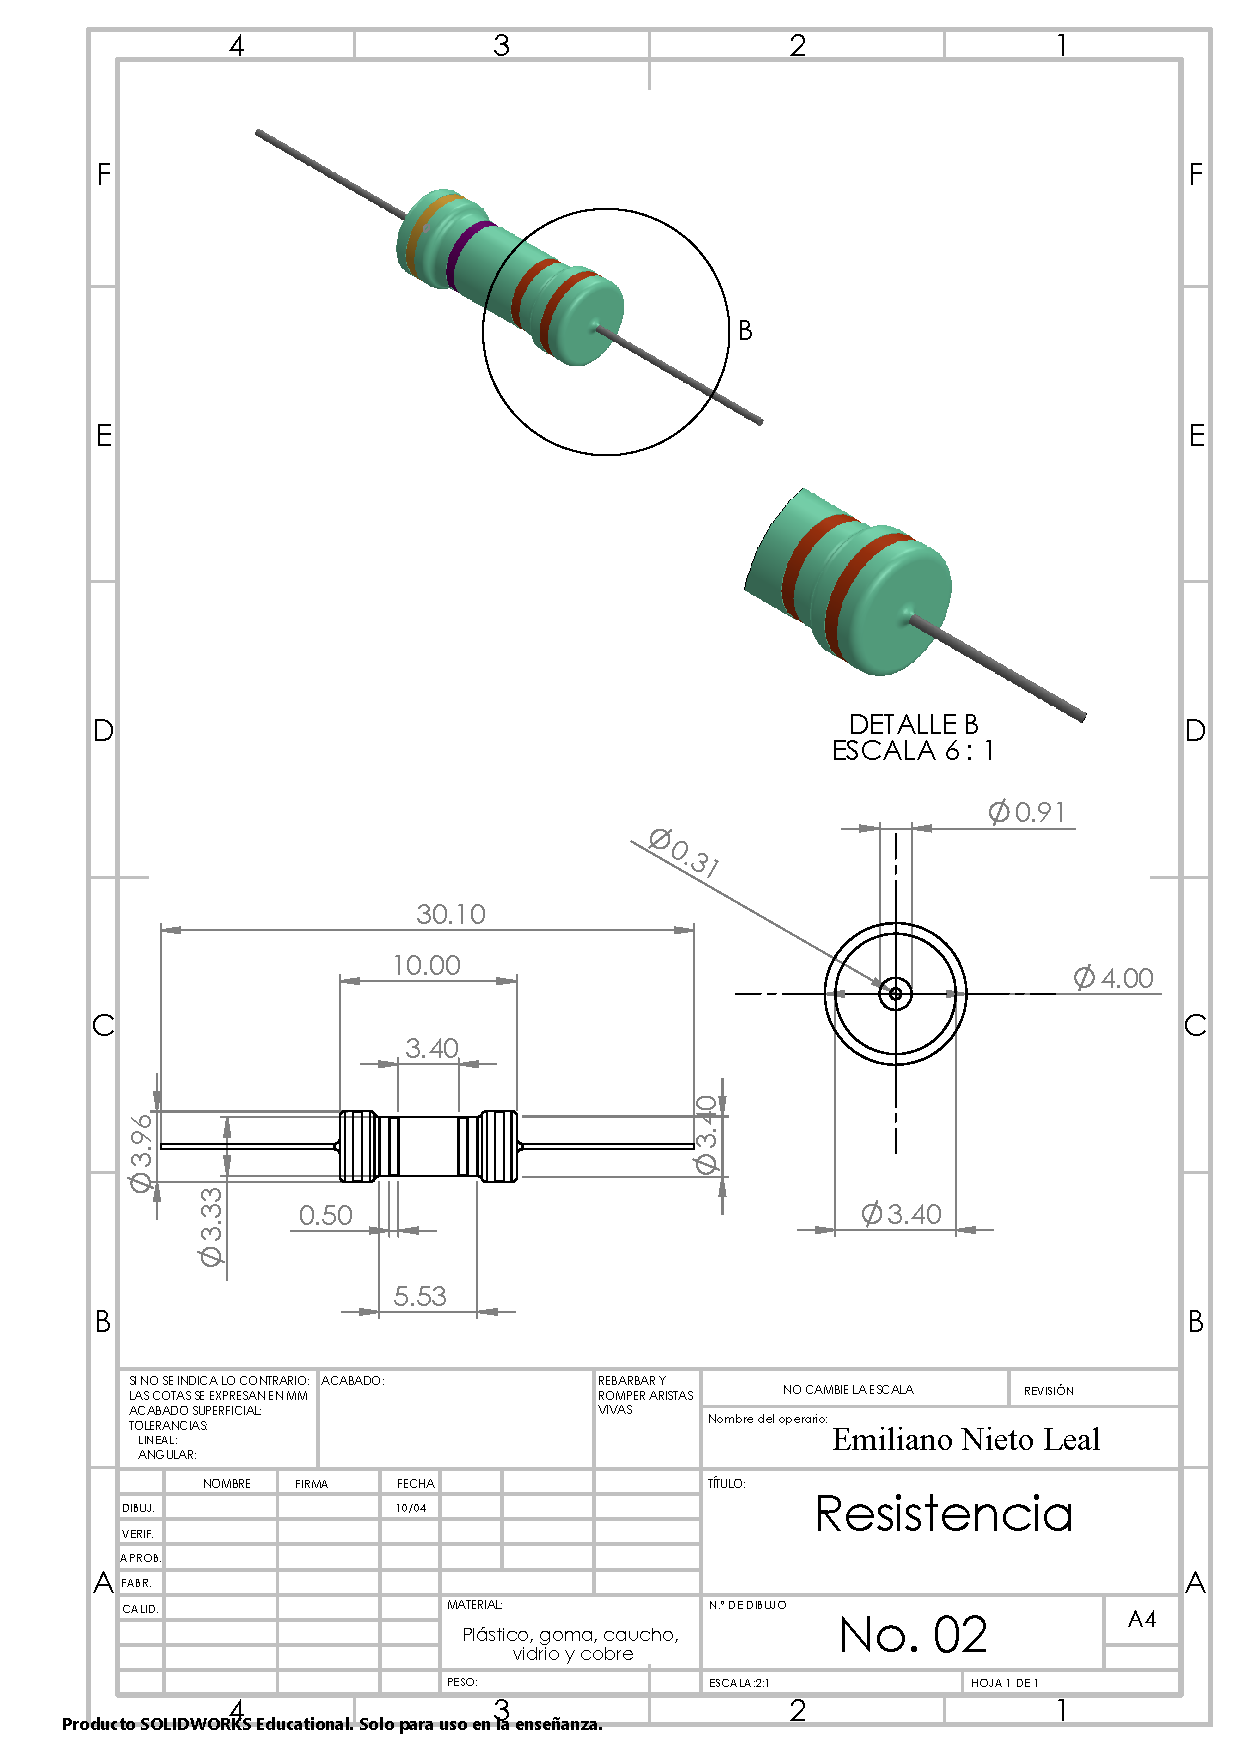
\includegraphics[trim = {1mm 1mm 1mm 1mm},clip,scale=0.3]{19/Img/resistenciaDibujo.pdf}
        \caption{Dibujo resistencia}
        \label{fig:Dibujo resistencia}
    \end{figure}
        
                \begin{figure}[H]
        \centering
        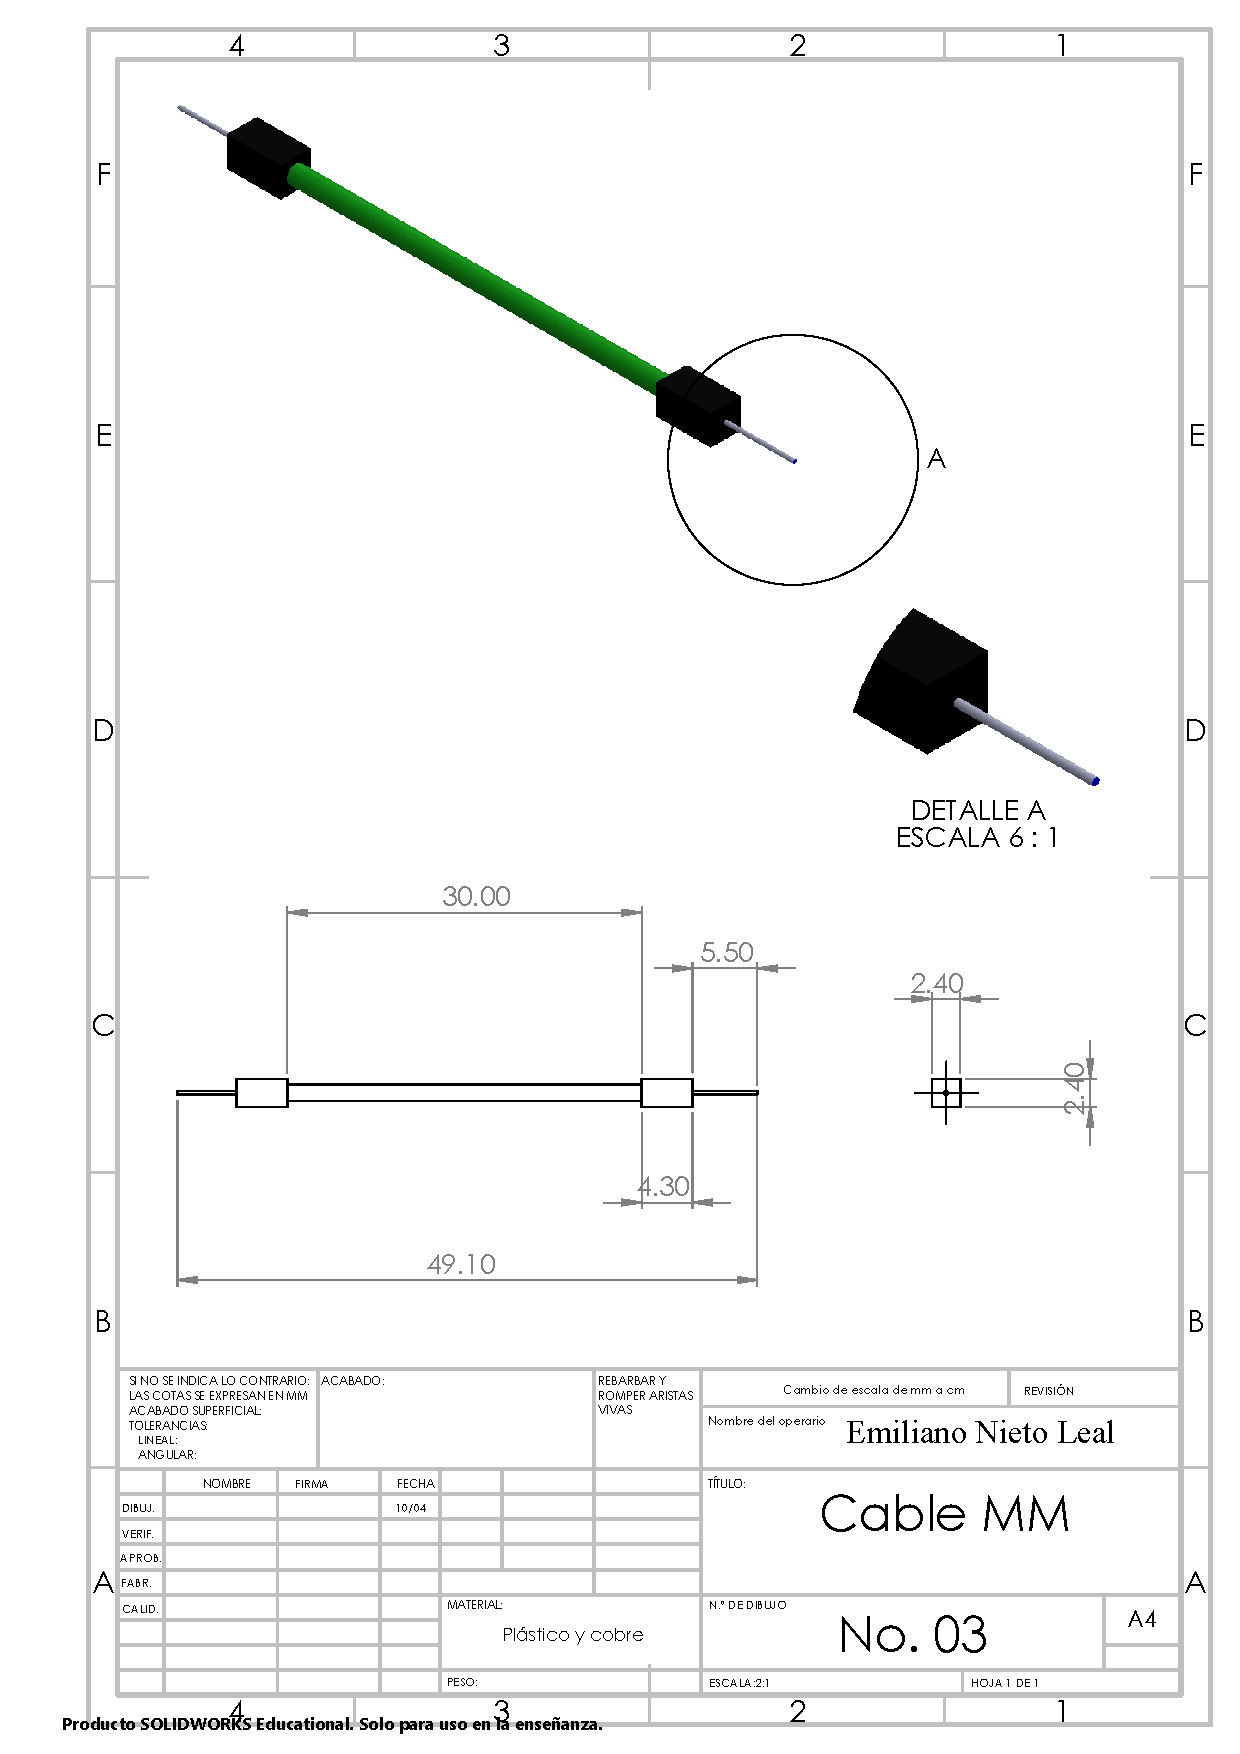
\includegraphics[trim = {1mm 1mm 1mm 1mm},clip,scale=0.3]{19/Img/cableMMDibujo.pdf}
        \caption{Dibujo CableMM}
        \label{fig:Dibujo cableMM}
    \end{figure}
    
                \begin{figure}[H]
        \centering
        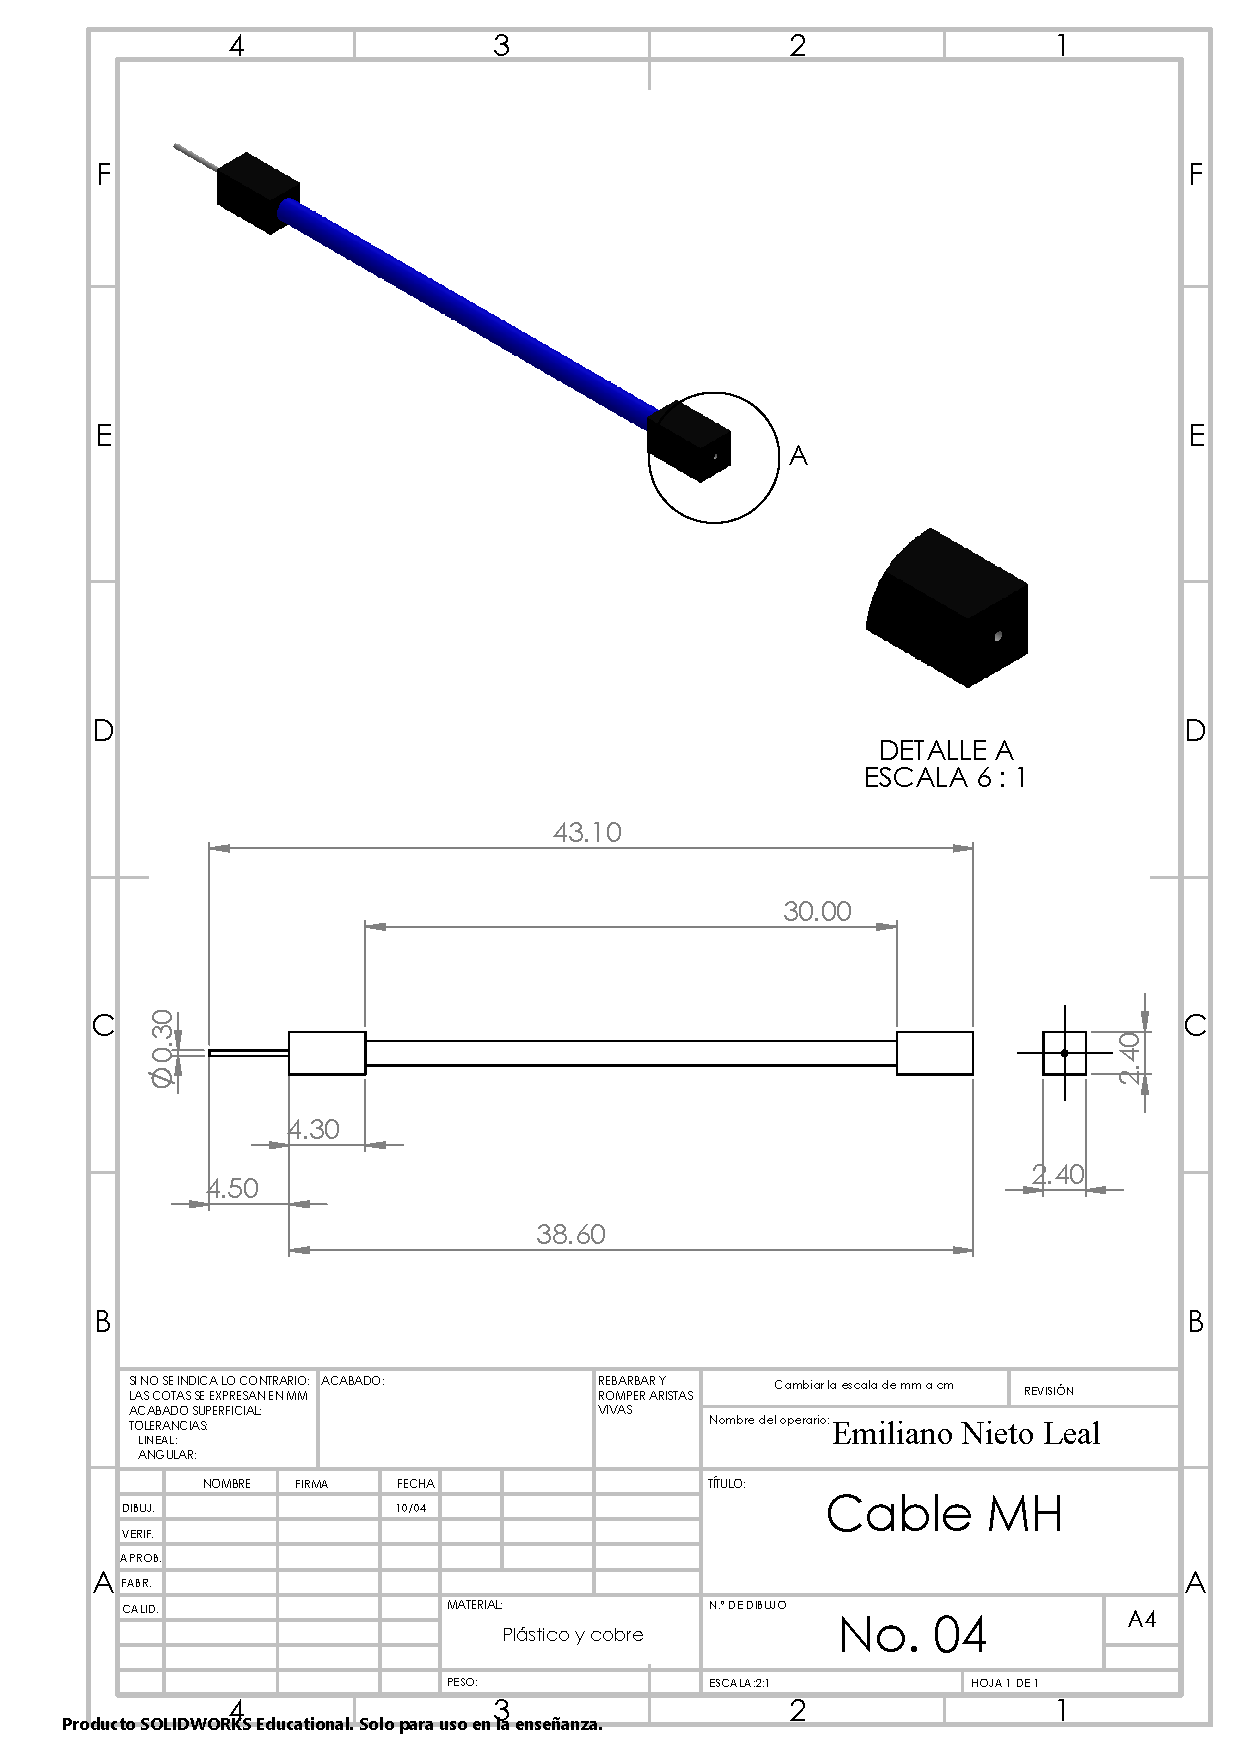
\includegraphics[trim = {1mm 1mm 1mm 1mm},clip,scale=0.3]{19/Img/cableMHDibujo.pdf}
        \caption{Dibujo CableMH}
        \label{fig:Dibujo cableMH}
    \end{figure}
    
                \begin{figure}[H]
        \centering
        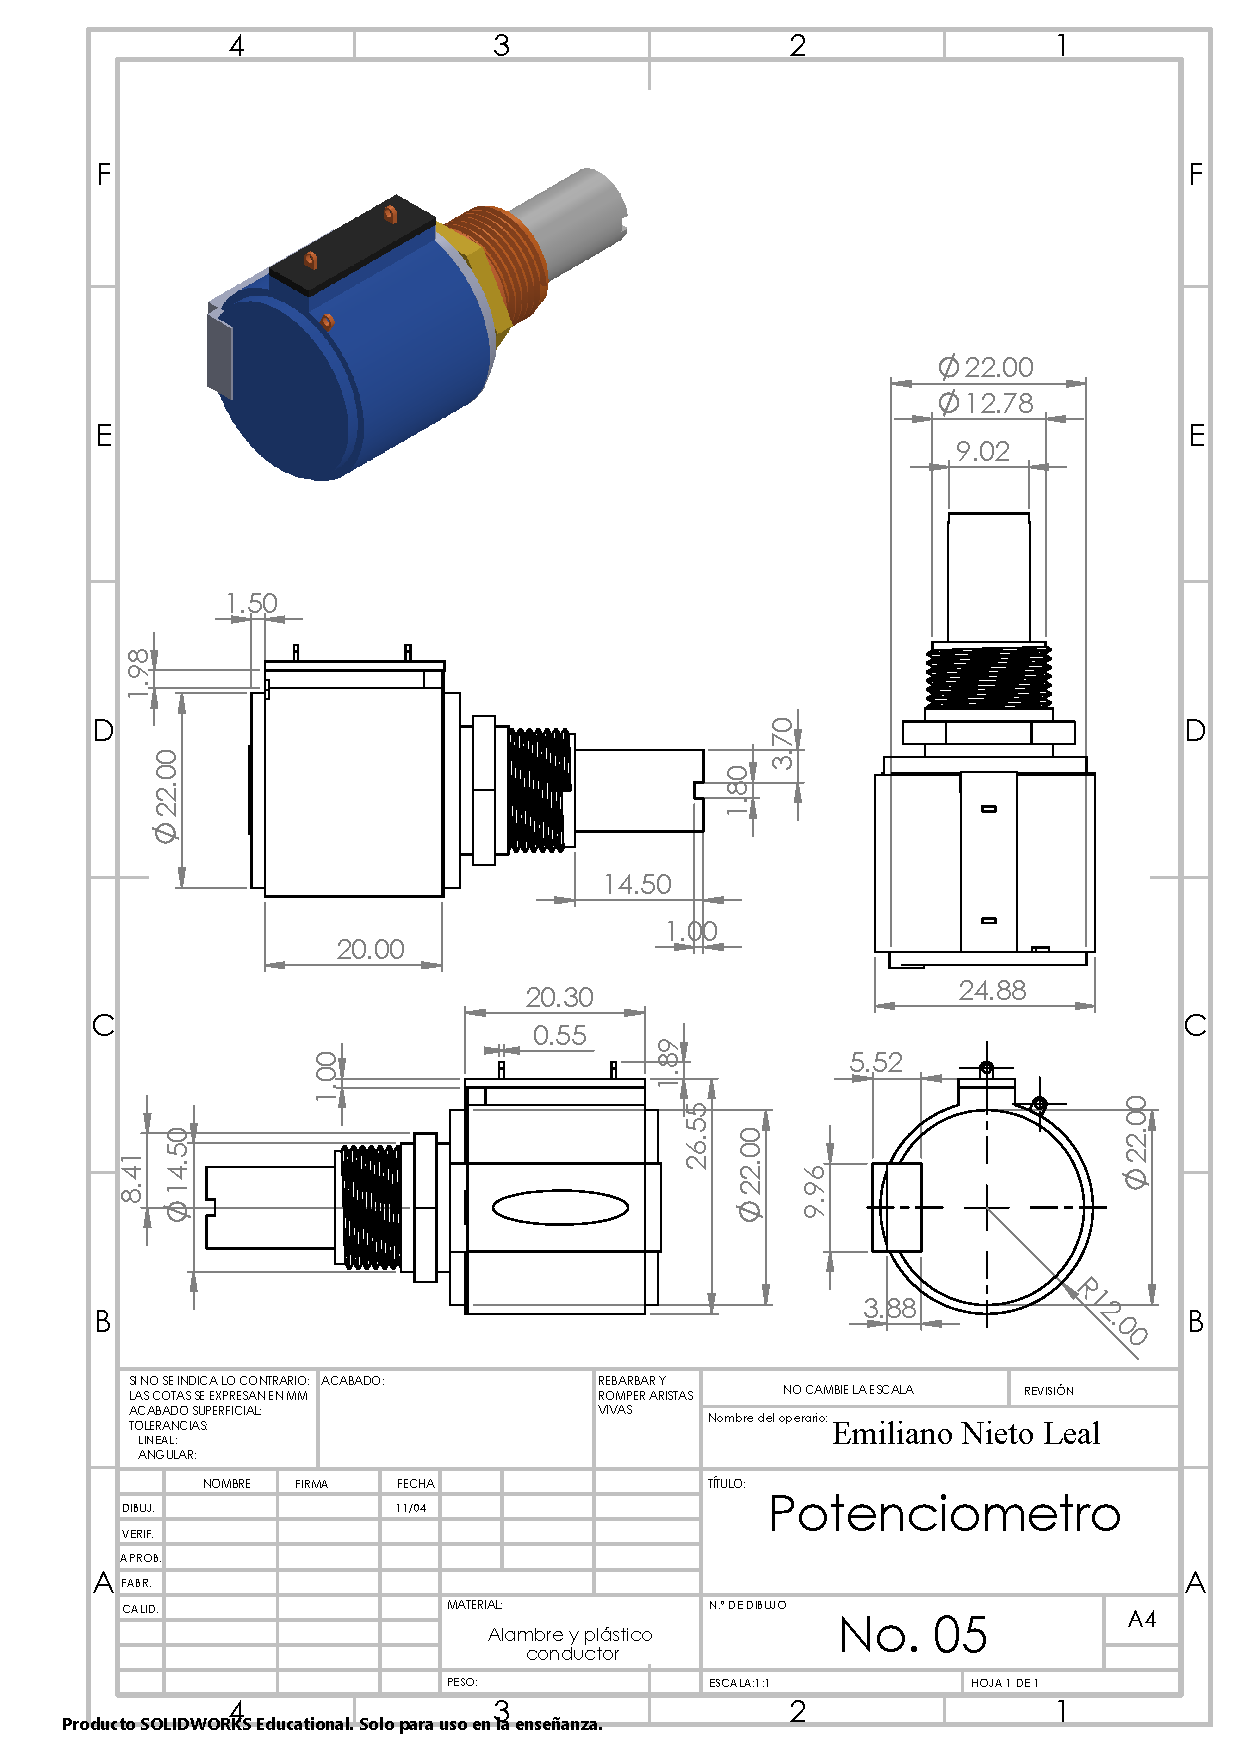
\includegraphics[trim = {1mm 1mm 1mm 1mm},clip,scale=0.3]{19/Img/potenciometroDibujo.pdf}
        \caption{Dibujo Potenciómetro}
        \label{fig:Dibujo Potenciómetro}
    \end{figure}

        \begin{figure}[H]
        \centering
        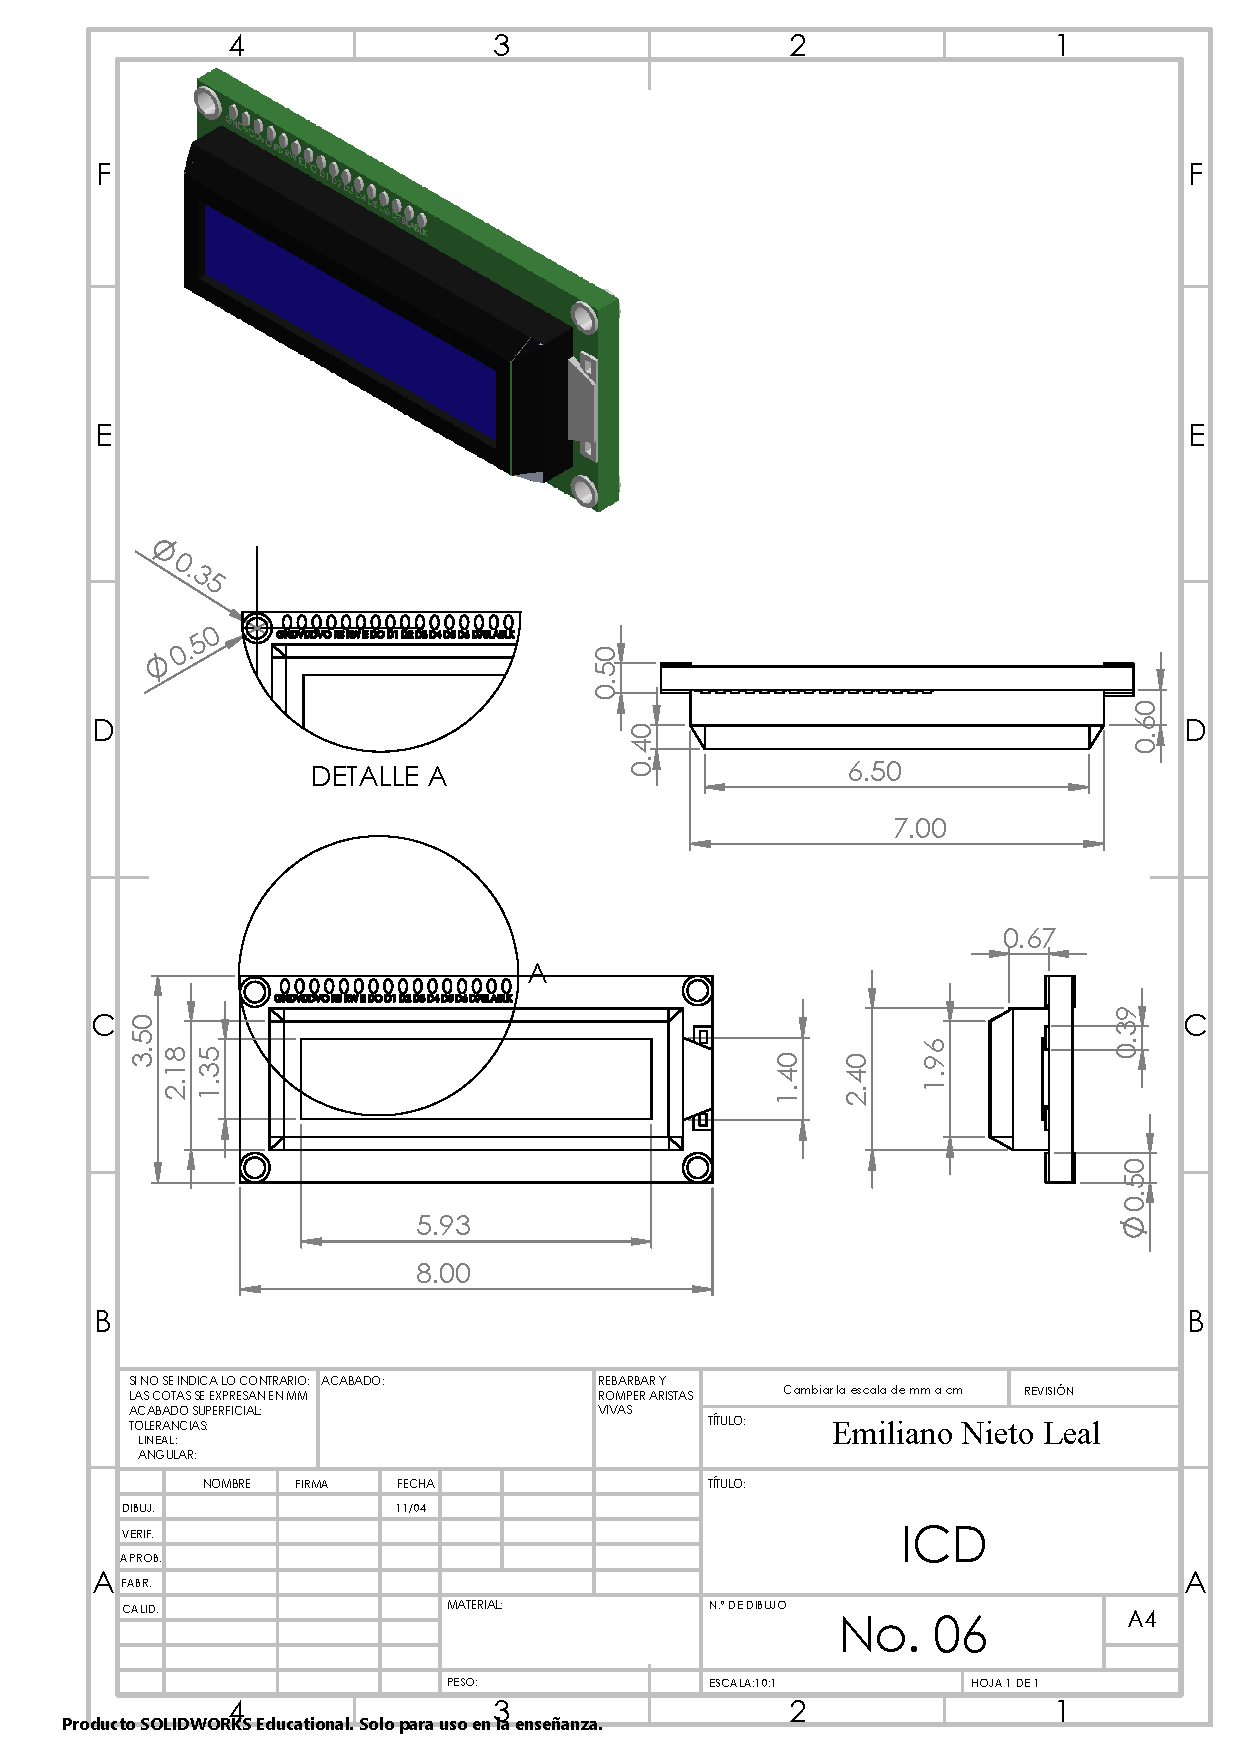
\includegraphics[trim = {1mm 1mm 1mm 1mm},clip,scale=0.3]{19/Img/icdDibujo.pdf}
        \caption{Dibujo LCD}
        \label{fig:Dibujo LCD}
    \end{figure}
                
                \begin{figure}[H]
        \centering
        \includegraphics[trim = {1mm 1mm 1mm 1mm},clip,scale=0.3]{19/Img/extensiónDibujo.pdf}
        \caption{Dibujo Extensión}
        \label{fig:Dibujo Extensión}
    \end{figure}
            
                \begin{figure}[H]
        \centering
        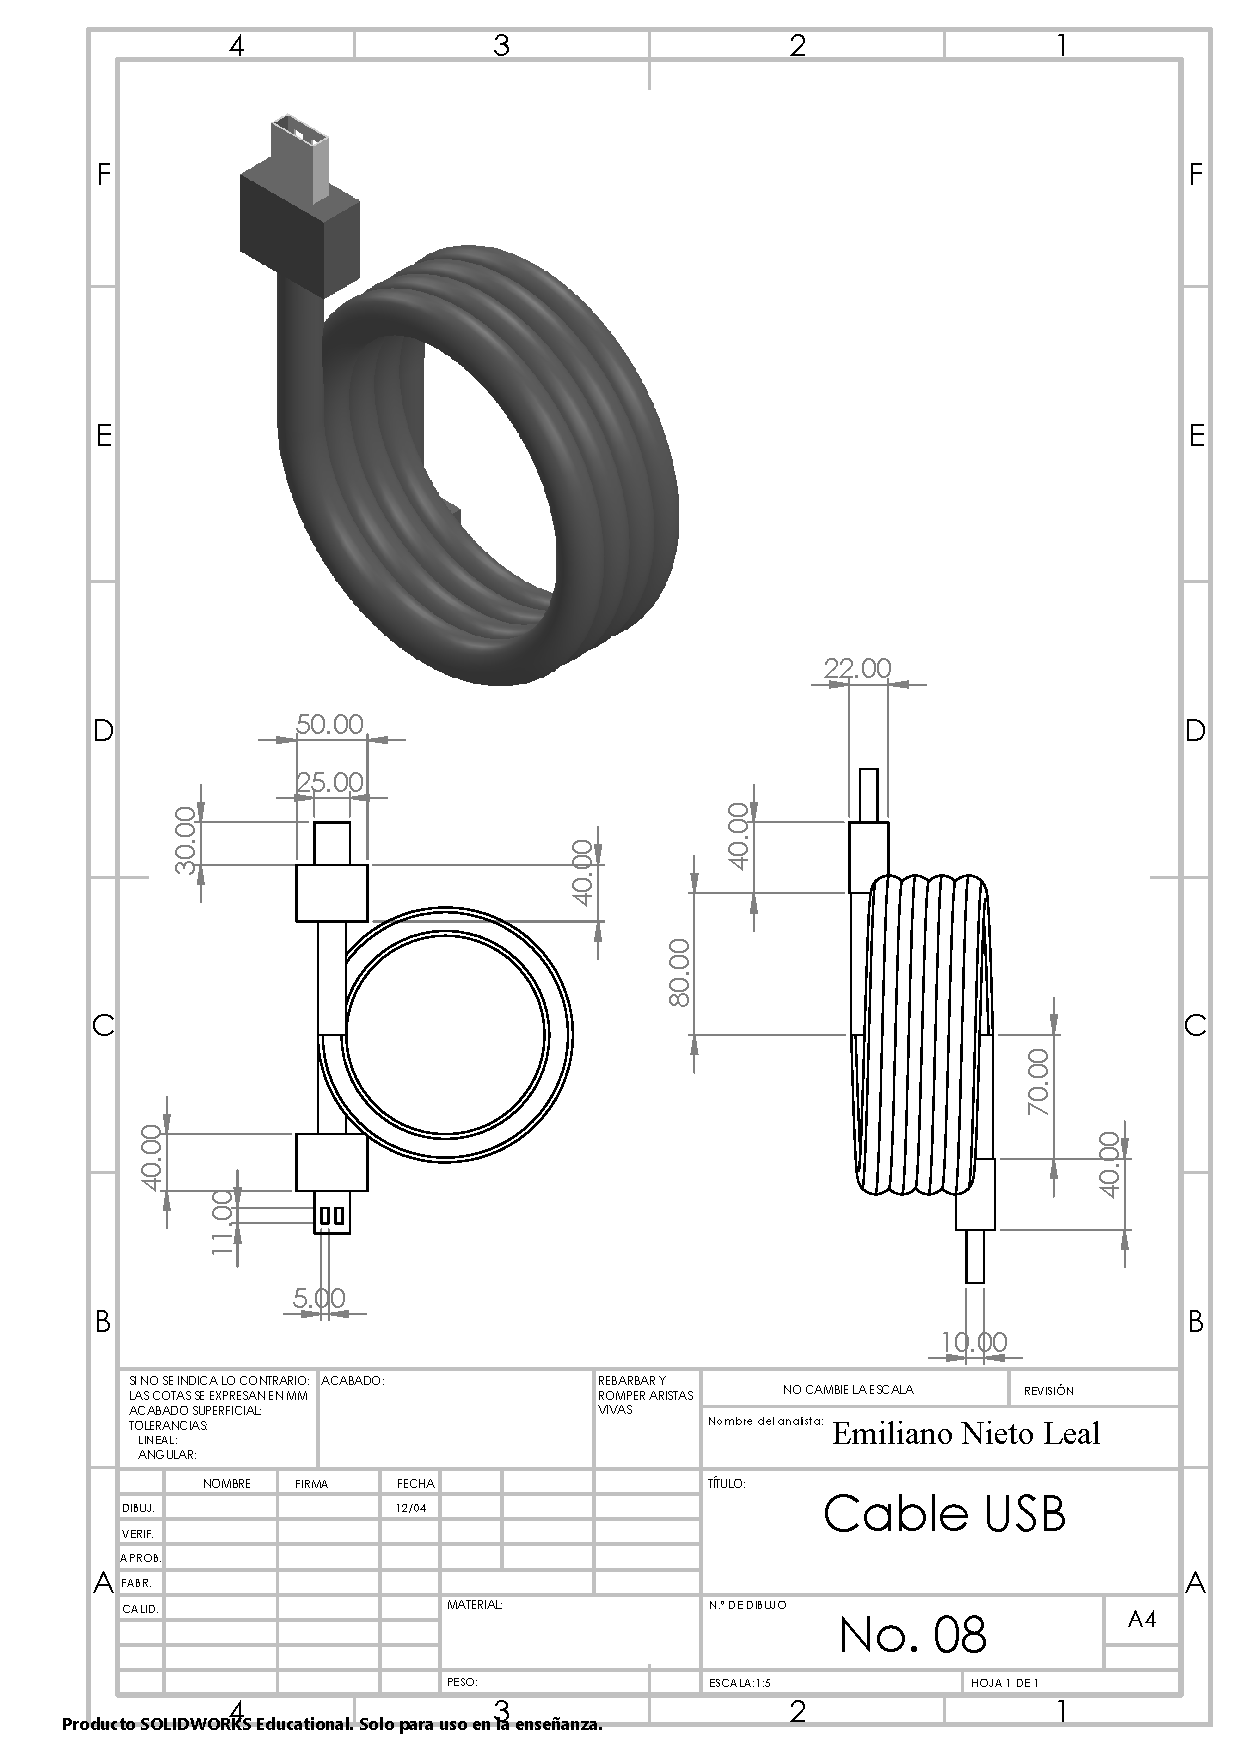
\includegraphics[trim = {1mm 1mm 1mm 1mm},clip,scale=0.3]{19/Img/cableUSBDibujo.pdf}
        \caption{Dibujo Cable USB}
        \label{fig:Dibujo CableUSB}
    \end{figure}
           
                \begin{figure}[H]
        \centering
        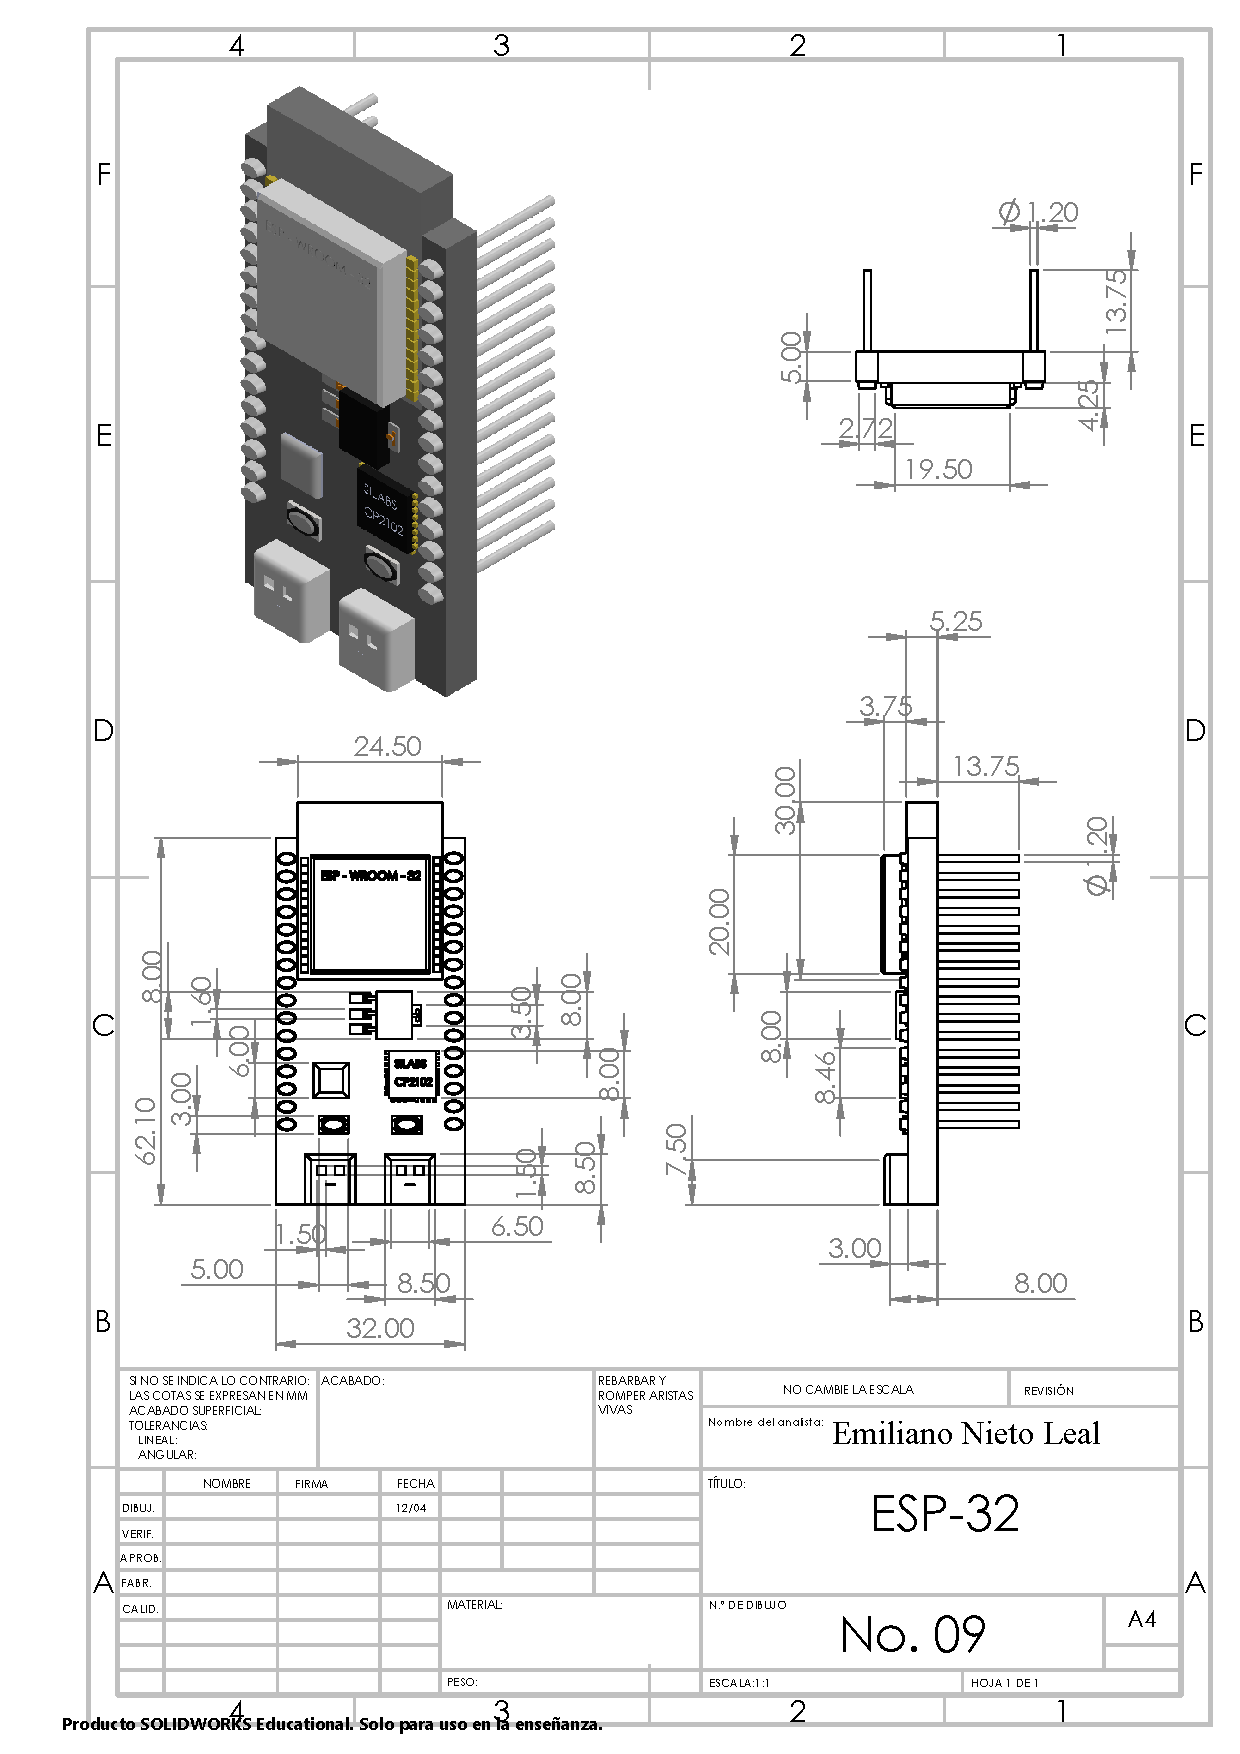
\includegraphics[trim = {1mm 1mm 1mm 1mm},clip,scale=0.3]{19/Img/esp32Dibujo.pdf}
        \caption{Dibujo ESP-32}
        \label{fig:Dibujo ESP-32}
    \end{figure}
    
    
                \begin{figure}[H]
        \centering
        \includegraphics[trim = {1mm 1mm 1mm 1mm},clip,scale=0.3]{19/Img/móduloI2CInterfazDibujo.pdf}
        \caption{Dibujo Módulo I2C Interfaz}
        \label{fig:modulodibujo}
    \end{figure}
           
         Estas piezas serán consideradas en la fabricación del manual para el operador, permitiendo conocer la forma de estas y el uso que se tendrá de las mismas.
         Cada pieza deberá encontrarse en un área accesible para el operador por lo que será necesario el uso de una herramienta para mantener los elementos con un orden y posición especifica, para la facilitación del operador, usando como ejemplo un tapete organizador, en donde se podrán colocar todo lo necesario para realizar el ensamble.\ref{fig:tapete}.
    
        \begin{figure}[H]
        \centering
        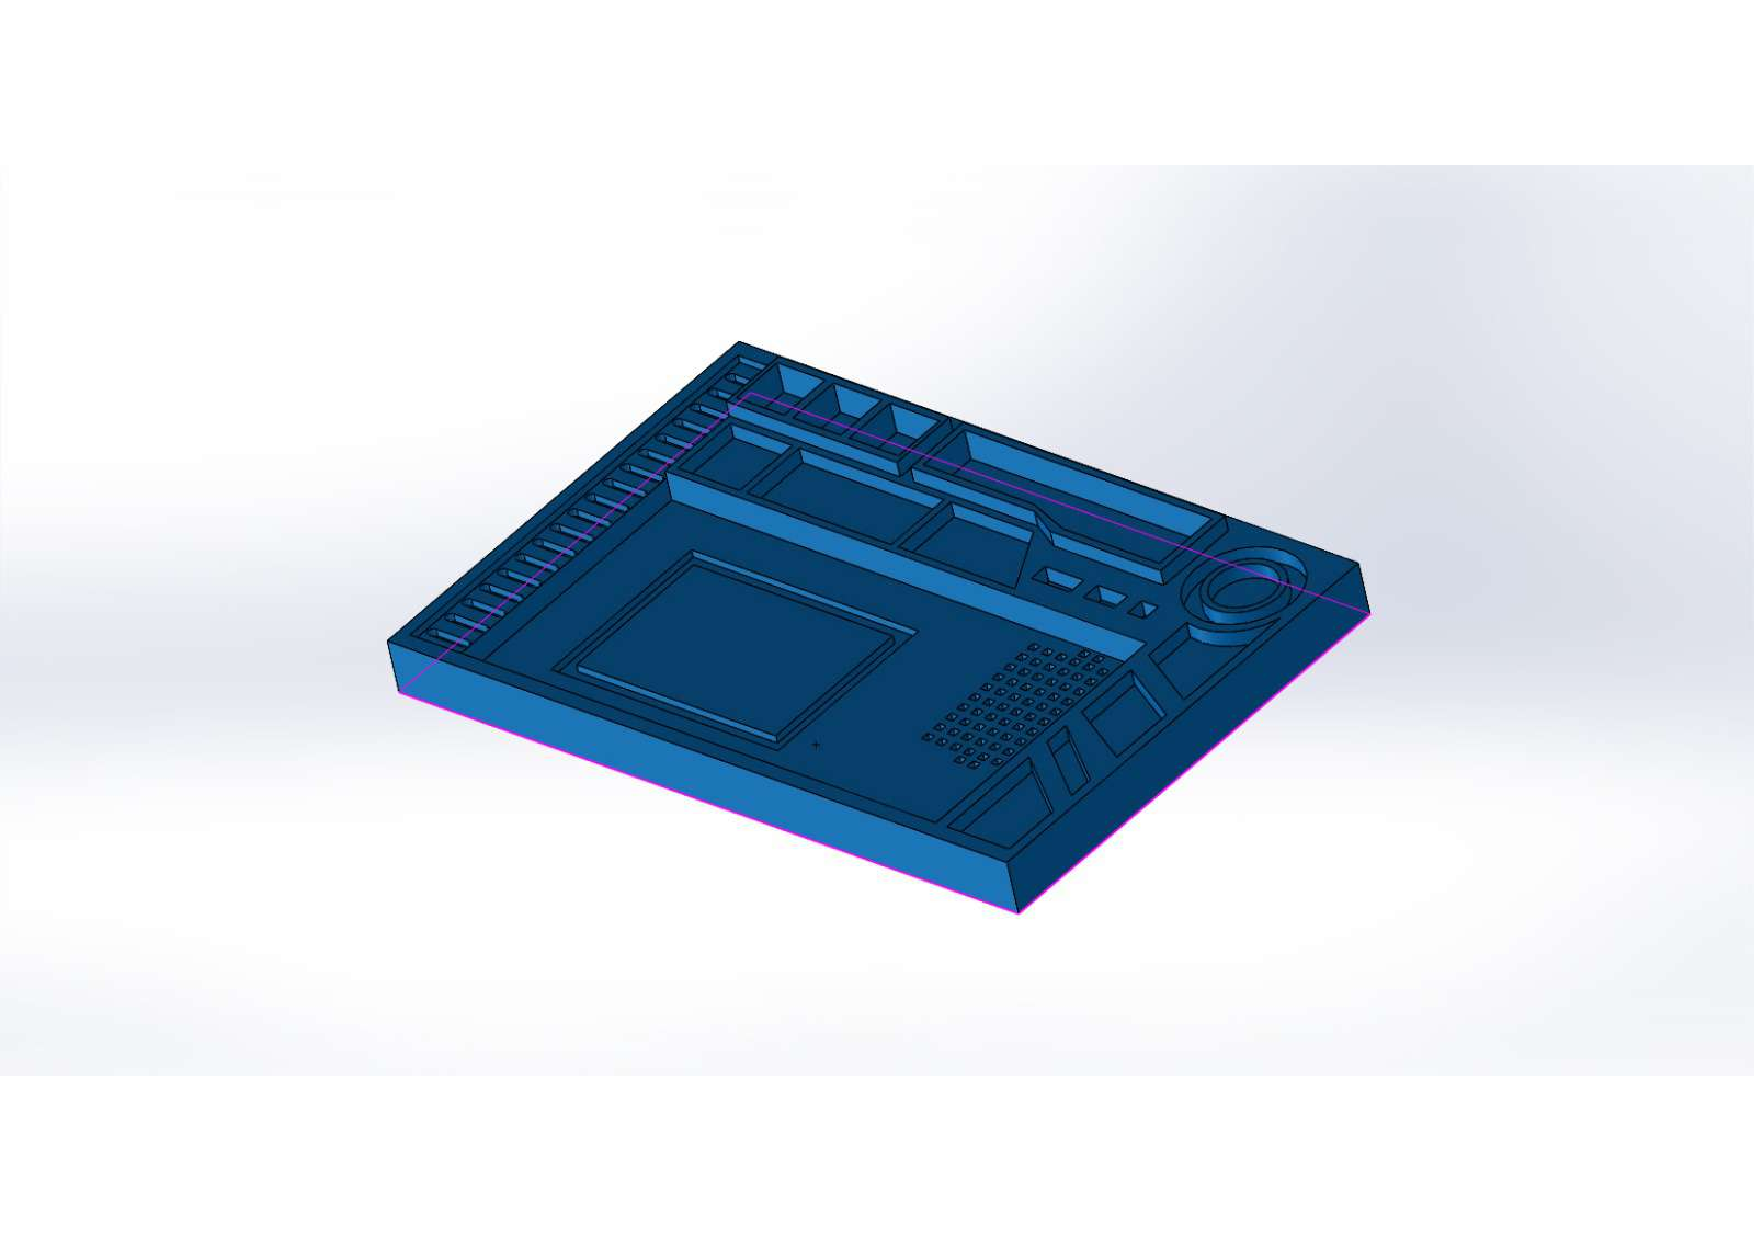
\includegraphics[trim = {65mm 55mm 65mm 55mm},clip,scale=0.5]{19/Img/tapeteOrganizadorFigura.pdf}
        \caption{Imagen del modelo 3D del Tapete organizador}
        \label{fig:tapete}
    \end{figure}
    
    \newpage
                \begin{figure}[H]
        \centering
        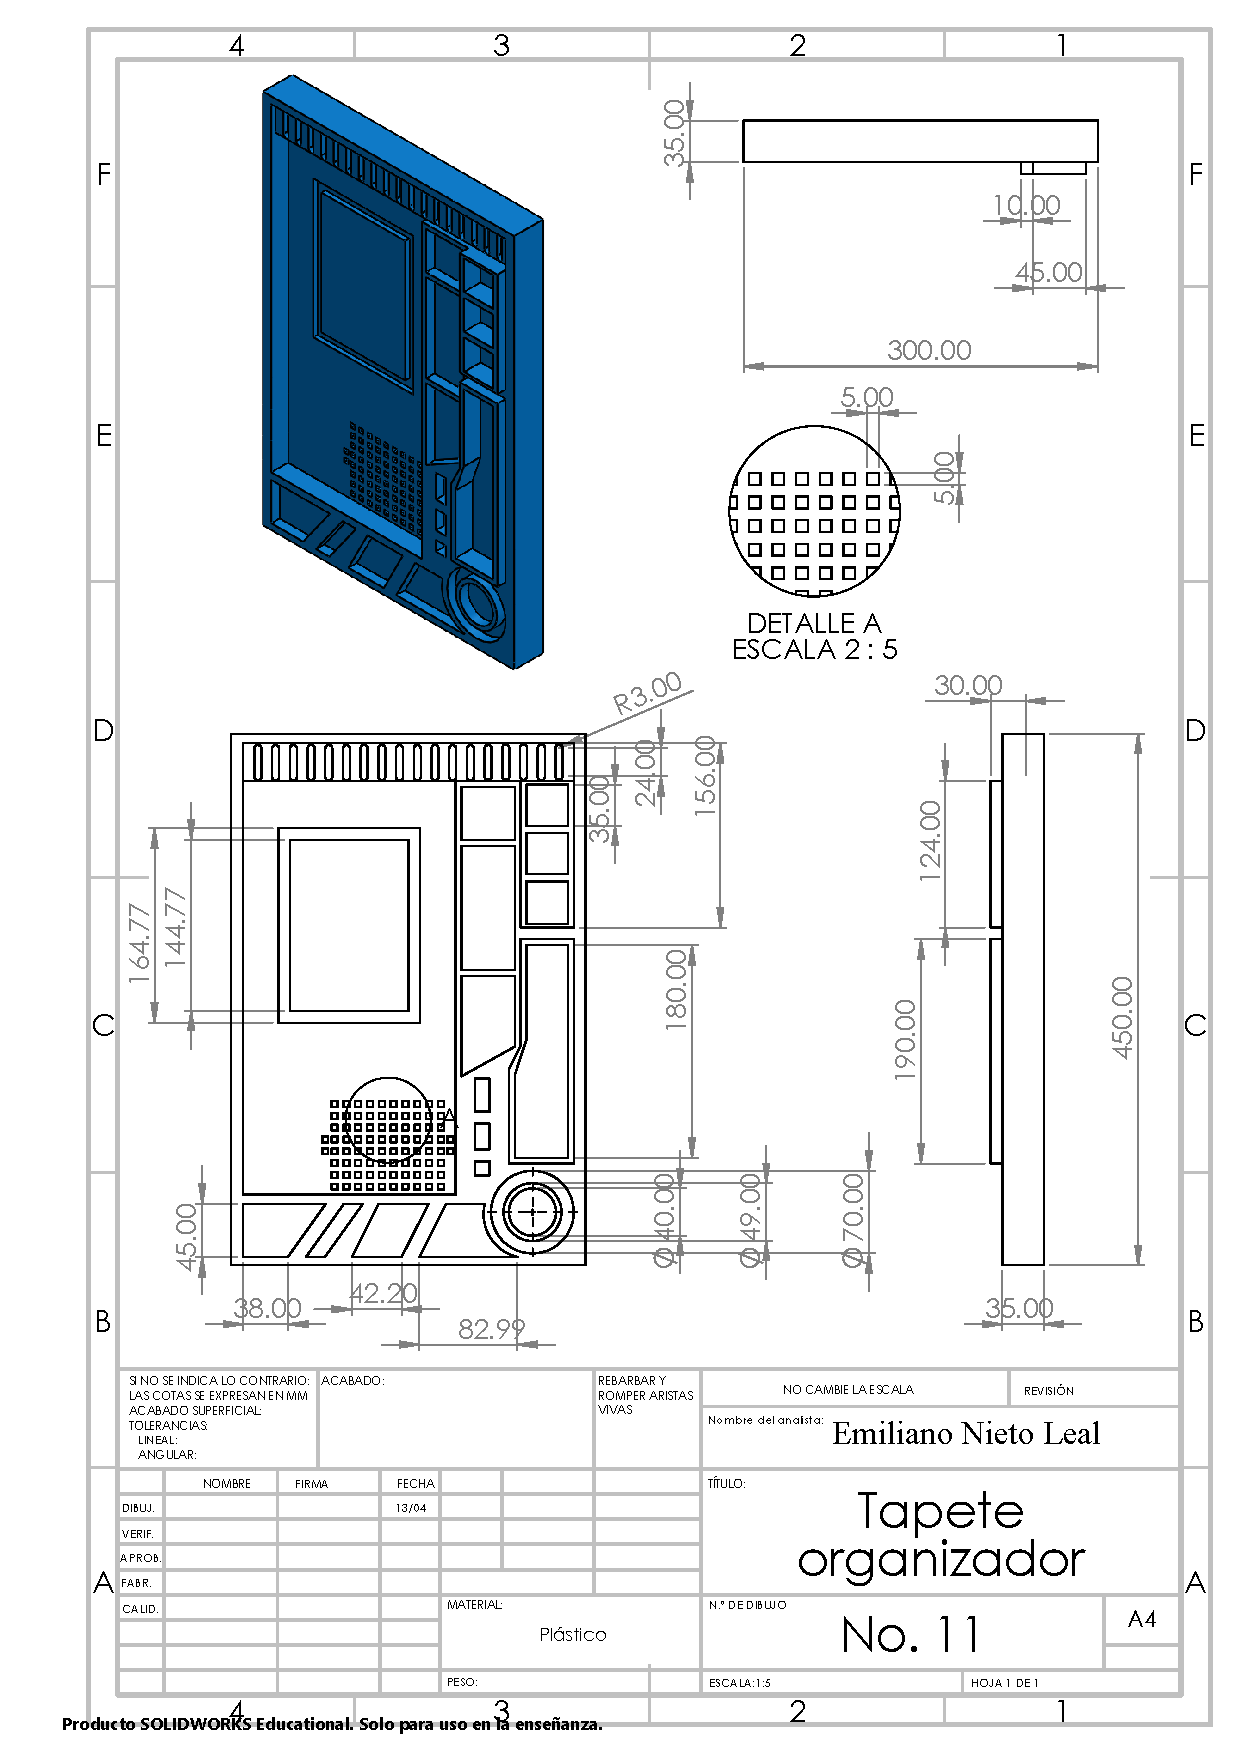
\includegraphics[trim = {1mm 1mm 1mm 1mm},clip,scale=0.35]{19/Img/tapeteOrganizadorDibujo.pdf}
        \caption{Dibujo Tapete Organizador}
        \label{fig:tapeteOrganizador}
    \end{figure}
    
        Después del operario entender los pasos y el proceso que se llevará acaba para realizar el ensamble se pedirá al operario que recuerde la cantidad de piezas a ocupar de cada material y cual es la función d esta en el circuito a ensamblar.
        \\Posterior a ello se pedirá que coloque todas las piezas y materiales necesarios para el proceso del ensamblaje en una posición adecuada alrededor del Tapete organizador como se presenta a continuación.\ref{fig:ensamblaje1}.
    \begin{figure}[H]
        \centering
        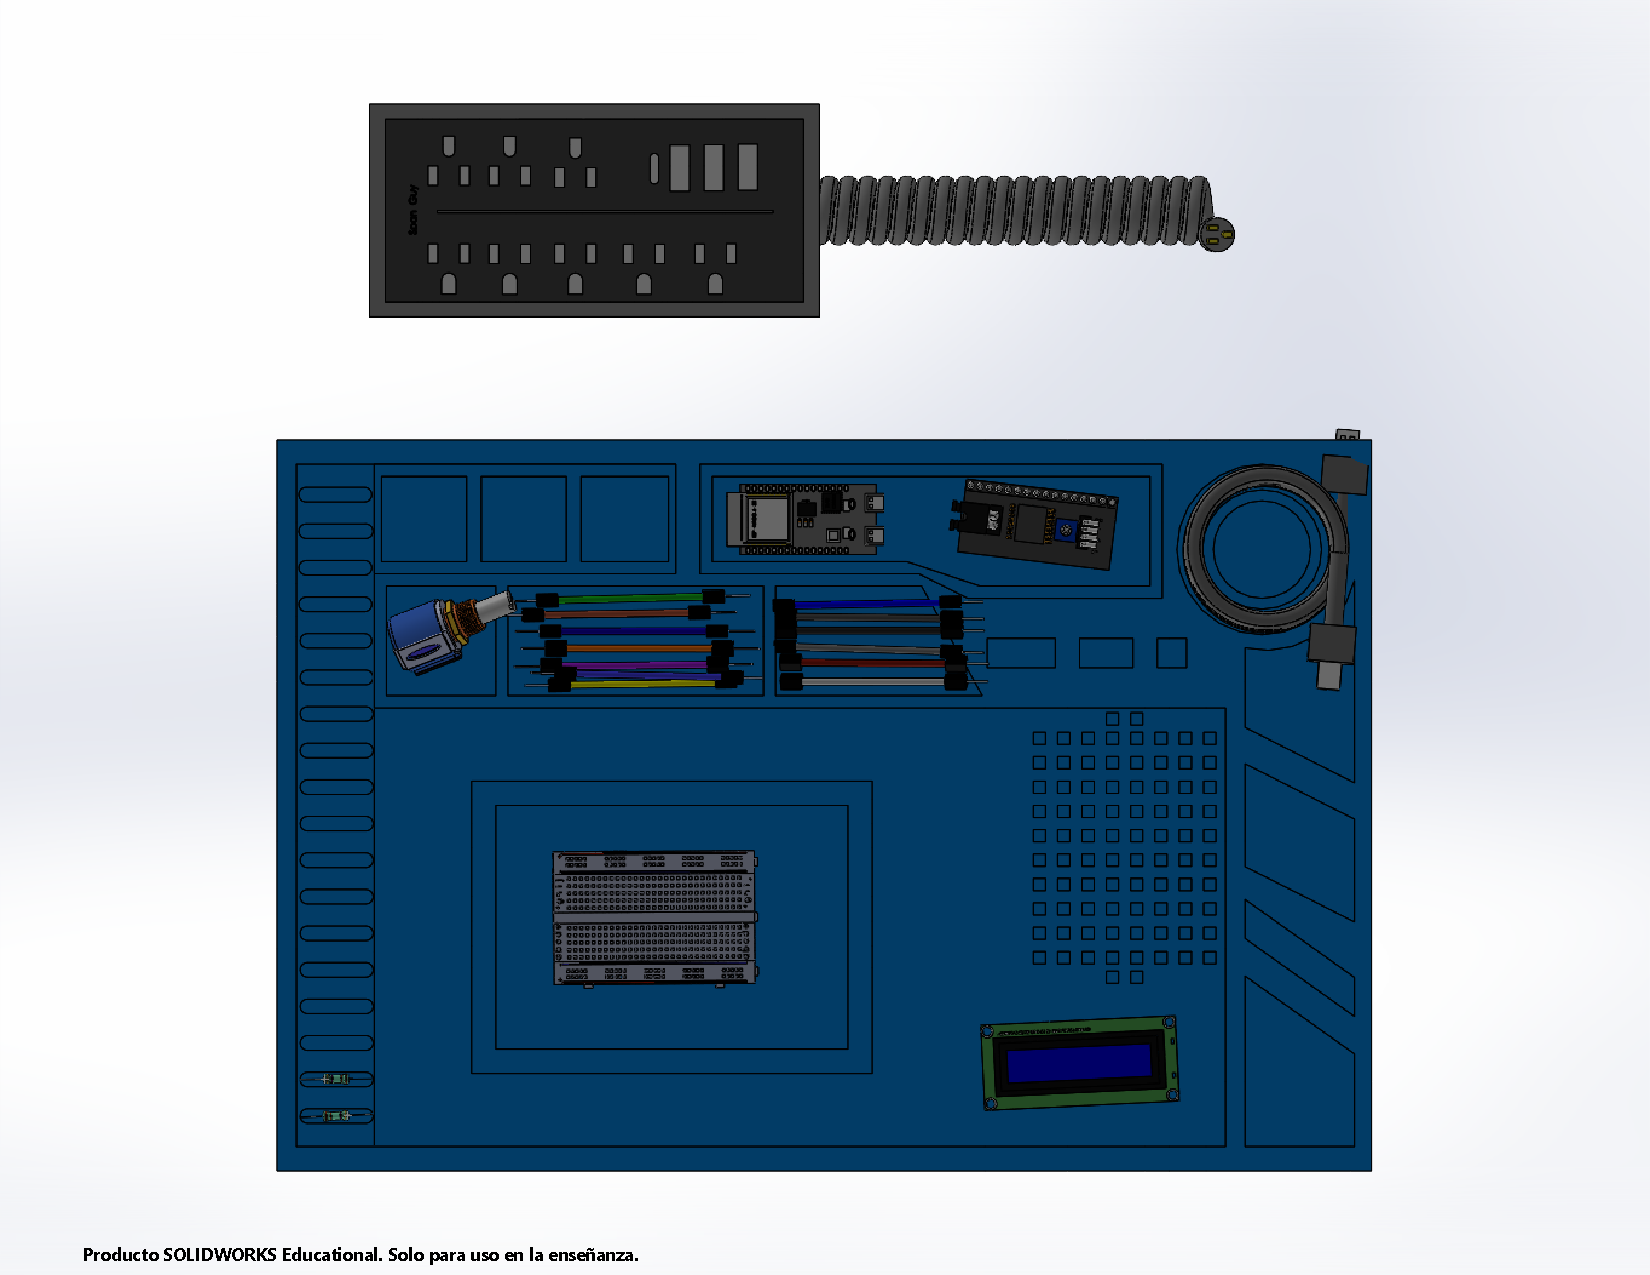
\includegraphics[trim = {55mm 15mm 40mm 20mm},clip,scale=0.38]{19/Img/ensamblaje1.pdf}
        \caption{Dibujo del Tapete Organizador con todas las piezas en orden}
        \label{fig:ensamblaje1}
    \end{figure}

        
         Después el operador dará inicio al proceso, con el inicio del operario el analista esta preparado con una cámara de vídeo con la cual se grabará la película en la cual podamos ver el proceso a realizar y la confirmación de haber realizado la prueba de calidad del producto.
        Al concluir este proceso con la confirmación de la prueba se terminará la primera observación, posteriormente el mismo analista deberá de llevar acabo una segunda observación para luego tomar el rol de operador, el cual igualmente ensamblara dos veces el circuito para obtener los valores  de cada observación usando la  fórmula para el valor esperado, el cual consiste en:
    
        \begin{equation}
        \label{eq1}
        (x1+x2+x3+........+xn)/n 
    \end{equation}
    
        para así poder obtener la media de todos los tiempos y concluir que este este es el tiempo esperado que se obtendrá al llevar acabo la metodología de tiempos continuos y de esta manera compararla con la siguiente metodología.

     \subsection{Determinación del tiempo estándar para que una persona competente realice el trabajo con marcha normal}
Para este momento ya se habrán estandarizado los tiempos en base a la muestra obtenida y de esta manera con el método y los materiales también ya estandarizados se podrá llegar a un valor exacto de tiempo en el que se debe de realizar el trabajo.
    %\subsection{Prepara tu documento}
    
    %Antes de que comiences a utilizar esta plantilla, es recomendable que prepare la información que contendrá en un archivo aparte. 
    %Ten preparadas tus gráficas, así como también las tablas aparte, para que sea más fácil integrarlo. 
    %Se recomienda fuertemente el uso de \textbf{formato Enhanced Metafile (.emf) para imágenes y gráficas} de resolución óptima. 
    %Finalmente, completa y organiza el contenido antes de darle el formato de esta plantilla. 
    
    %\subsection{Acrónimos y Abreviaciones}

    
    %Los acrónimos y abreviaciones deberán ser definidos únicamente la primera vez que aparecen en el texto, esto para que el lector entienda lo que significan.
    
    \newpage
    \section{Resultados y discusión}

    \subsection{Desarrollo de la guía del Plan de Emergencia}

    En esta guía de emergencia se desea generar e implementar las estrategias de seguridad que todo alumno, trabajador y  persona que se pueda encontrar dentro de las instalaciones debe de seguir en caso de encontrarse con diversos riesgos dentro del Instituto Tecnológico de Querétaro; detectando tanto a los miembros capacitados para seguir estas estrategias, los materiales pertinentes, conocimiento de instalaciones y todo conocimiento que se debe de tomar en cuenta para mitigar las consecuencias antes, durante y después de que ocurra esa situación de emergencia.
    
    Antes que todo se debe de poseer la información básica y los datos generales del Tecnológico Nacional, estando relativamente cerca del centro de Querétaro el Instituto Tecnológico de Querétaro o también llamado "ITQ" forma parte de un sistema de educación superior que es para muchos considerado la mejor escuela de Ingenierías del país, el cual tiene diversos campus a lo largo del país. Para esta guía nos centraremos en el campus centro del estado de Querétaro, a continuación en la figura \ref{fig:mapaITQ} se mostraran todos los datos básicos referentes al tecnológico.

\begin{figure}[H]
    \centering
    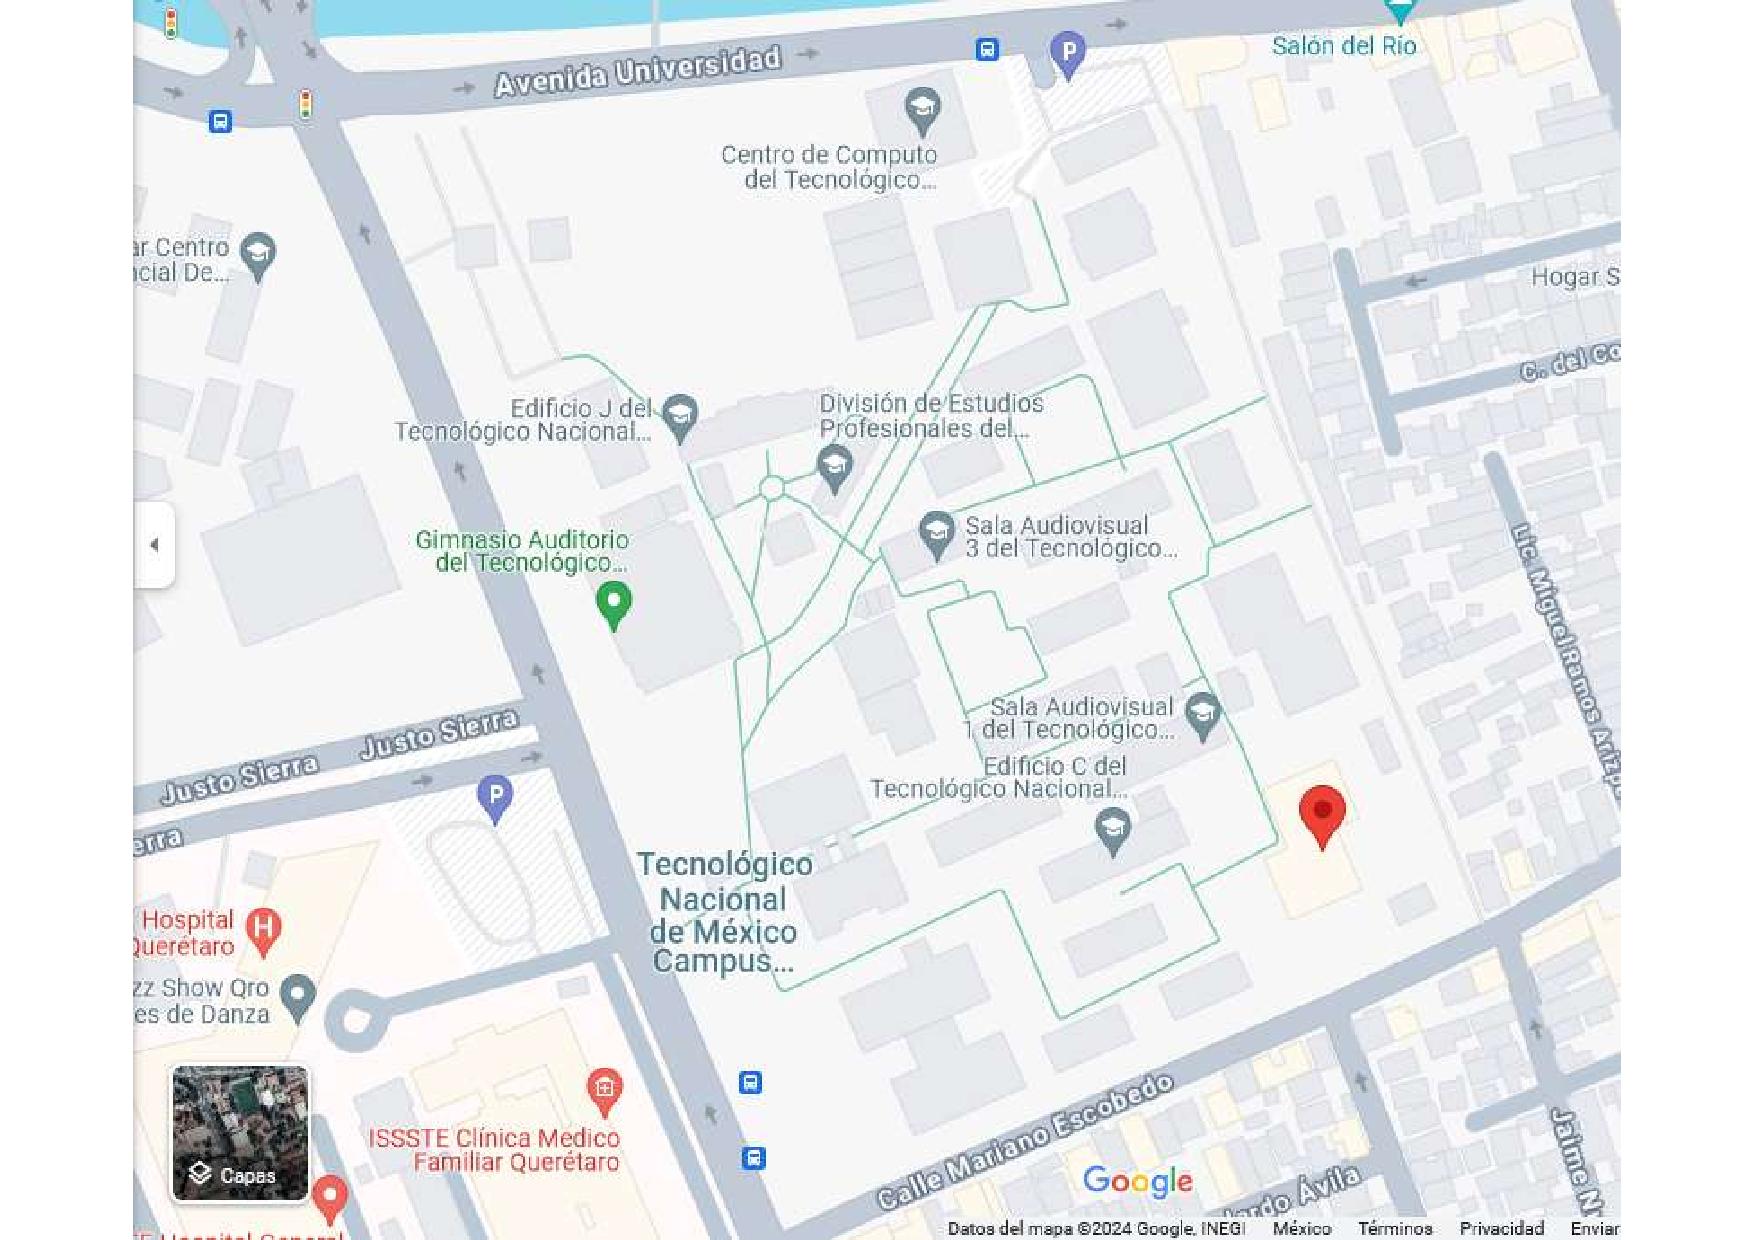
\includegraphics[scale=0.32]{19/Img/mapaITQ.pdf}
    \caption{Tecnológico Nacional de México, Instituto Tecnológico de Querétaro, Av. Tecnológico S/N, Centro Histórico, Centro, 76000 Santiago de Querétaro, Qro., Número telefónico: 442 227 4400 Ext. 4423}
    \label{fig:mapaITQ}
\end{figure}
    
    Aquí también se presenta la imagen satelital del Instituto Tecnológico de Querétaro, con el cual se puede observar con mayor facilidad las divisiones de los edificios dentro del inmueble \ref{fig:mapaITQ-2}.

    \begin{figure}[H]
    \centering
    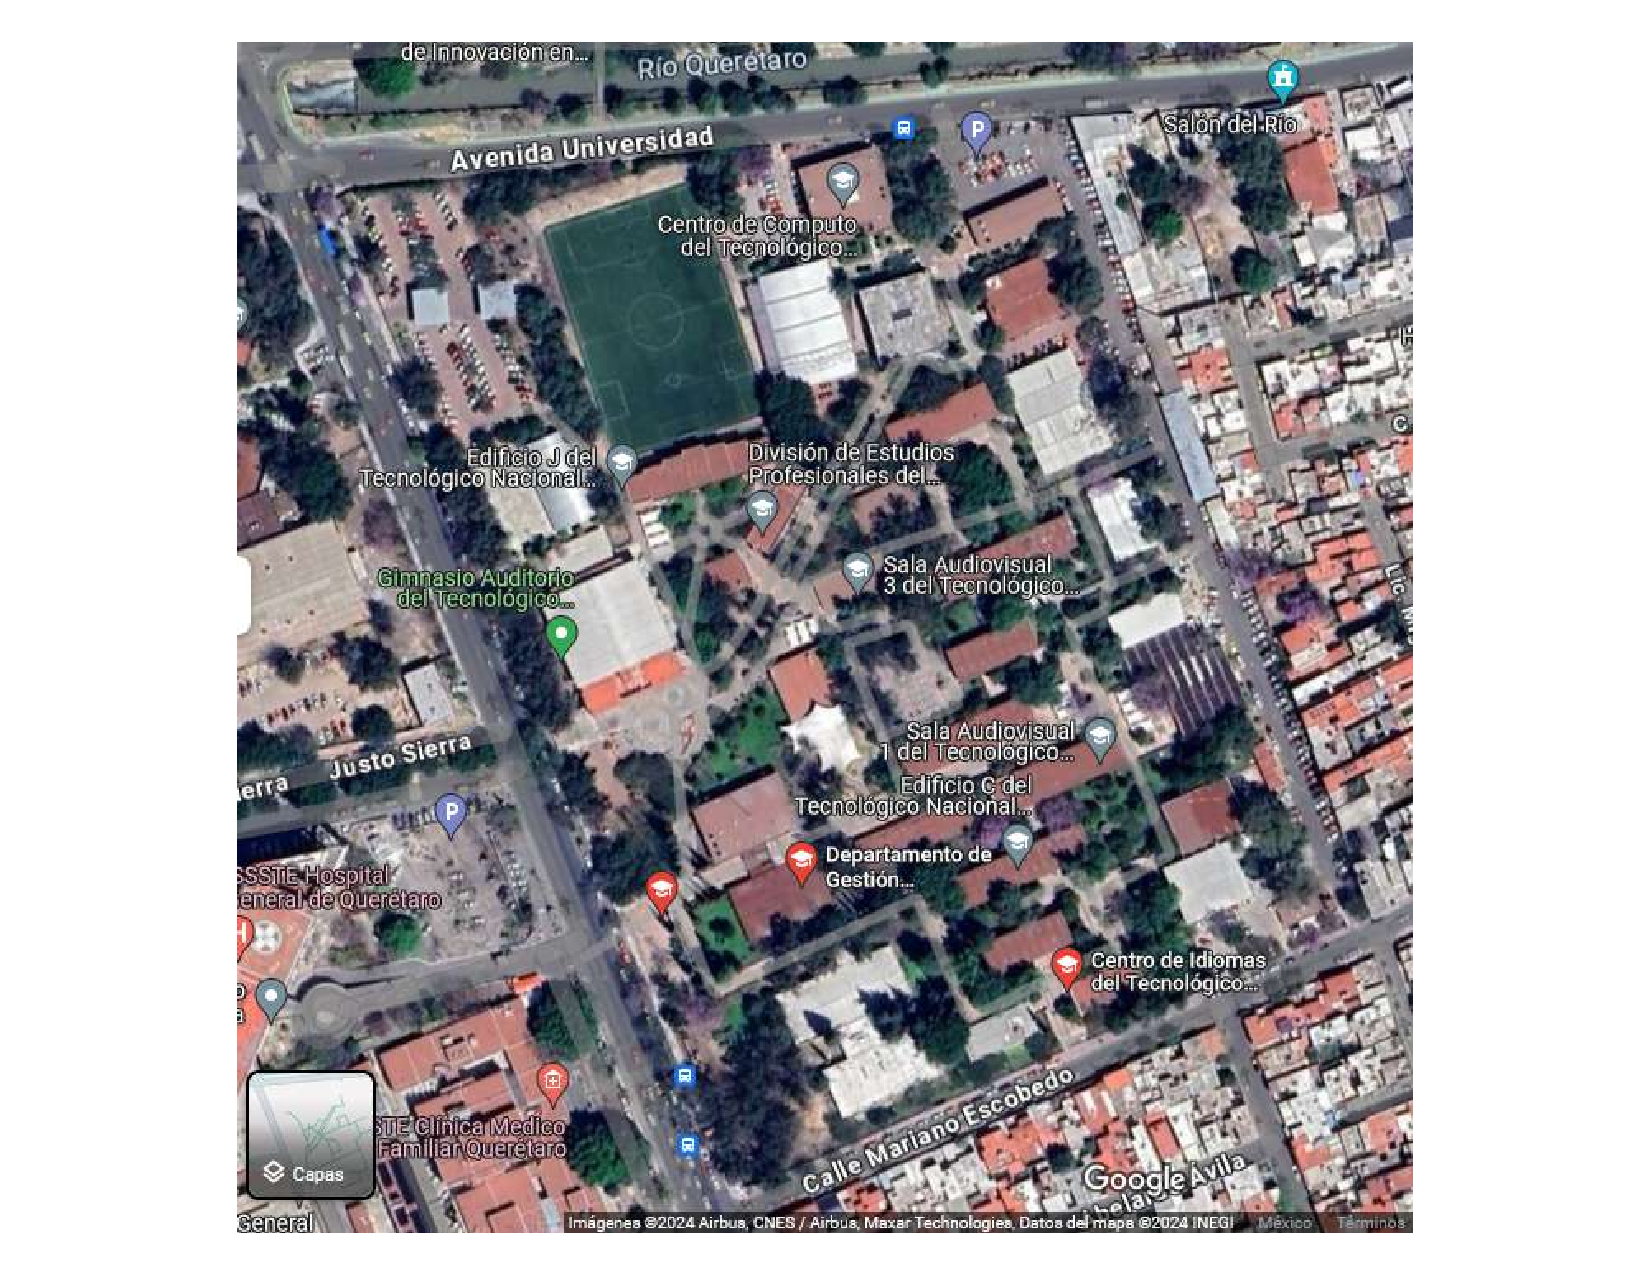
\includegraphics[scale=0.32]{19/Img/mapaITQ2.pdf}
    \caption{Imagen Satelital del Instituto Tecnológico Nacional de Querétaro.}
    \label{fig:mapaITQ-2}
\end{figure}

 \subsubsection{Análisis de riesgo}

 Al considerar el edificio del clases C como el área de desarrollo del ensamble, se realizó una revisión general a este y a sus edificios más cercanos con el propósito de observar no solo los riesgos más propensos a generarse, tanto dentro de los edificios, afuera de este, en la institución en general o incluso fuera de esta; para ello se generó un diagrama \ref{fig:diagrama-1} que especifica el como identificar y reaccionar ante alguna situación de riesgo, usando también como base la tabla \ref{tab:riesgos} para identificar el grado de riesgo que esta situación posee.

    \begin{figure}[H]
    \centering
    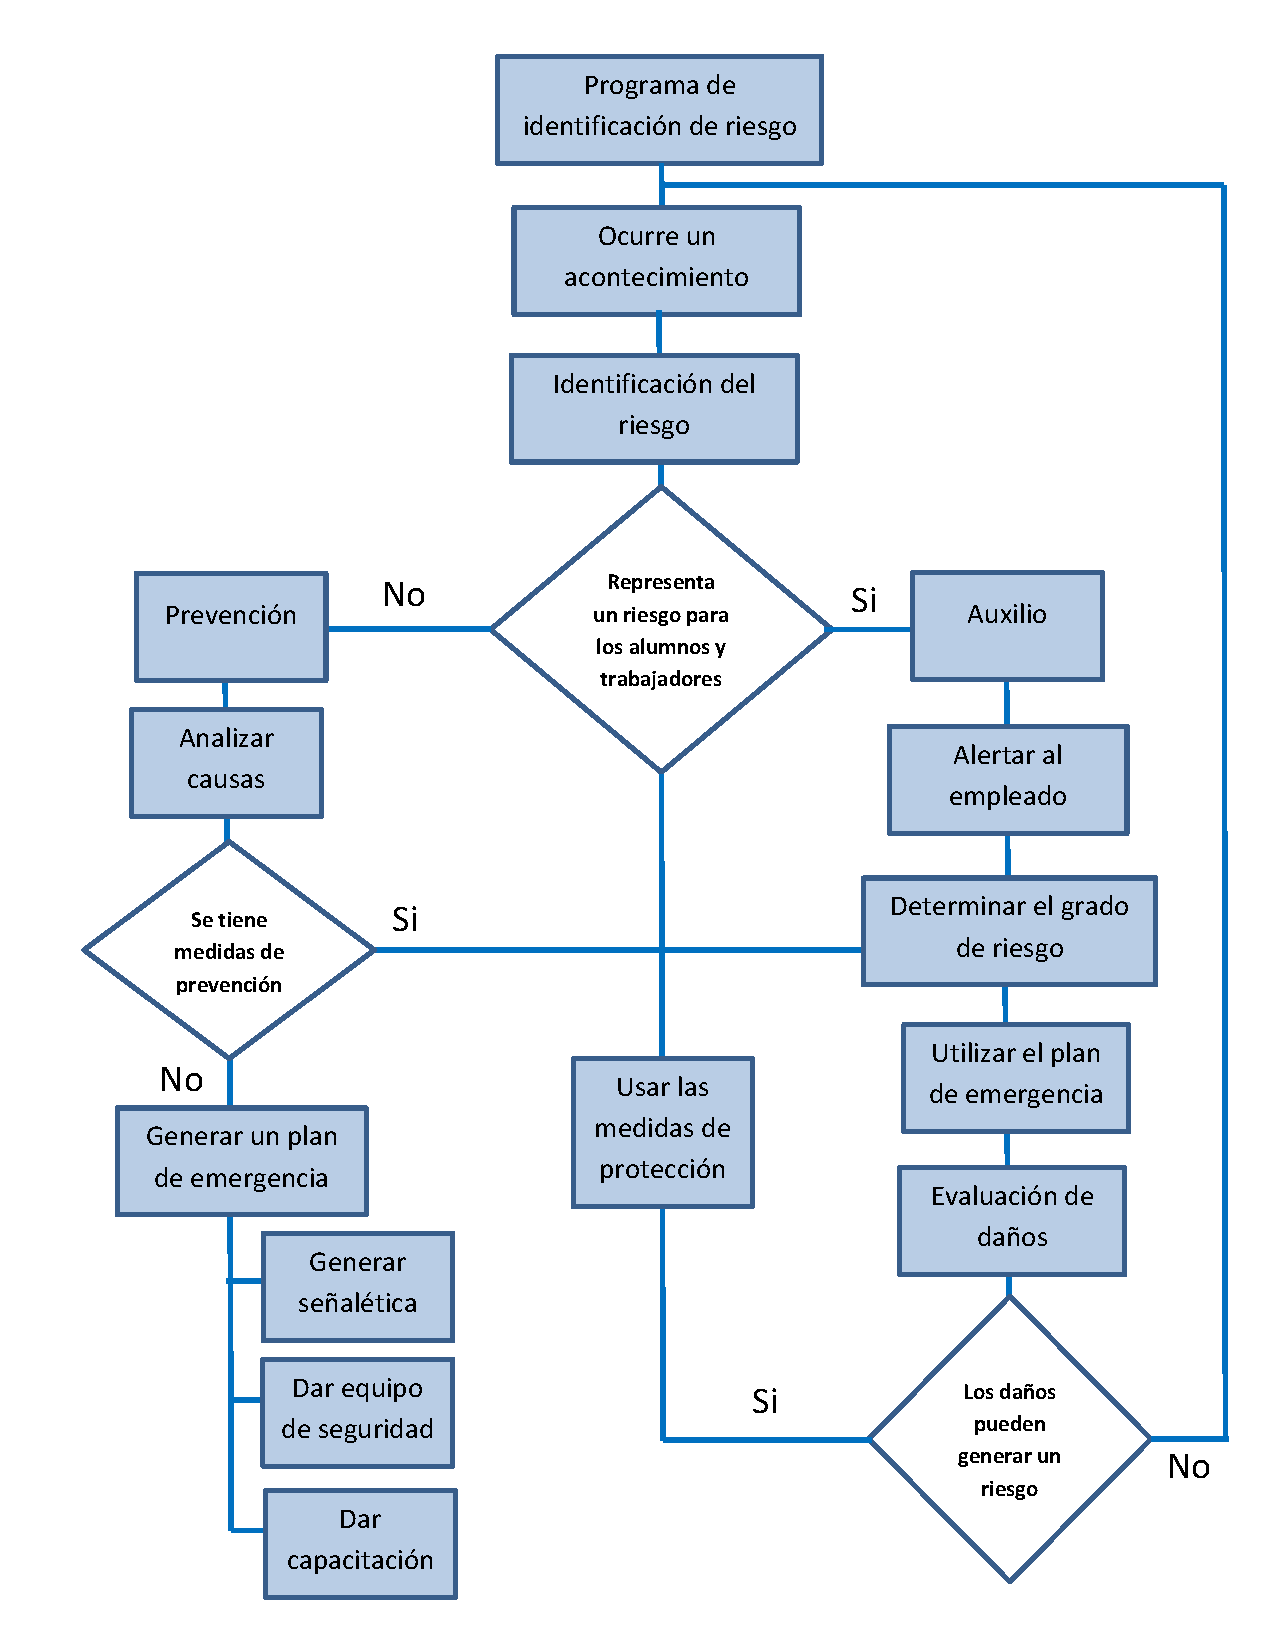
\includegraphics[scale=0.32]{19/Img/diagrama1.pdf}
    \caption{Diagrama para la identificación de riesgos y acciones}
    \label{fig:diagrama-1}
    \end{figure}

     \subsubsection{Riesgos internos}

     Descrito por la RAE el riesgo es definido como cada contingencia que se puede generar por un contrato de seguro o para cualquier daño en general que pueda ocurrir \cite{RAE2}, dicho de otro es cualquier situación que pueda poner en peligro la estabilidad de un ente o una persona. Siendo los riesgos internos aquellos daños que se generan dentro de la empresa o entidad, y cuyo responsable la mayoría del tiempo son trabajadores internos o como se maneja el funcionamiento de esta, siendo los mas probables presentados en la tabla de riesgos internos \ref{fig:riesgosInt}. 
     \\Para separar los riesgos en general en base a su nivel de peligrosidad se han desarrollado diversas ayudas visuales para los trabajadores, y así entender el grado de riesgo que ocupa cada problema, siendo el uso de tablas el más frecuente entre estos, siendo muy conocidos tablas de relación directa y las tablas 5x5, la cual será la usada para la guía de emergencia, que tomara como base tanto el impacto de la emergencia como las probabilidades de que ocurra, junto con un conjunto de colores que va cambiando de verde claro, verde oscuro, amarillo, naranja, rojo claro y rojo oscuro en base al mayor impacto que este suceso puede generar:
     \begin{table}[H]
    \centering
    \caption{Tabla de riesgos 5x5 en base al impacto y probabilidad de los sucesos}
    \begin{tabular}{p{1.4cm} p{1.7cm} p{0.8cm} p{1.5cm} p{1cm} p{1cm}}
    \hline
    \multicolumn{6}{c}{Impacto}\\
    {Probabilidad}\\
    \hline
        -- & Insignificante (1) & Menor (2) & Significativo (3)  & Mayor (4) & Severo (5)\\
    \hline
        (5) Casi seguro & Medio (5) & Alto (10)  & Muy alto (15) & Extremo (20) & Extremo (25) \\
    \hline
        (4) Probable & Medio (4) & Medio (8)  & Alto (12) & Muy alto (16) & Extremo (20) \\
    \hline
        (3) Moderado & Bajo (3) & Medio (6)  & Medio (9) & Alto (12) & Muy Alto (15) \\
    \hline 
        (2) Poco Probable & Muy Bajo (2) & Bajo (4)  & Medio (6) & Medio (8) & Alto (10) \\
    \hline
        (1) Bajo & Muy Bajo (1) & Muy bajo (2)  & Bajo (3) & Medio (4) & Medio (5) \\
    \hline
    \end{tabular}
    \label{tab:riesgos}
\end{table}
 
    \begin{figure}[H]
        \centering
        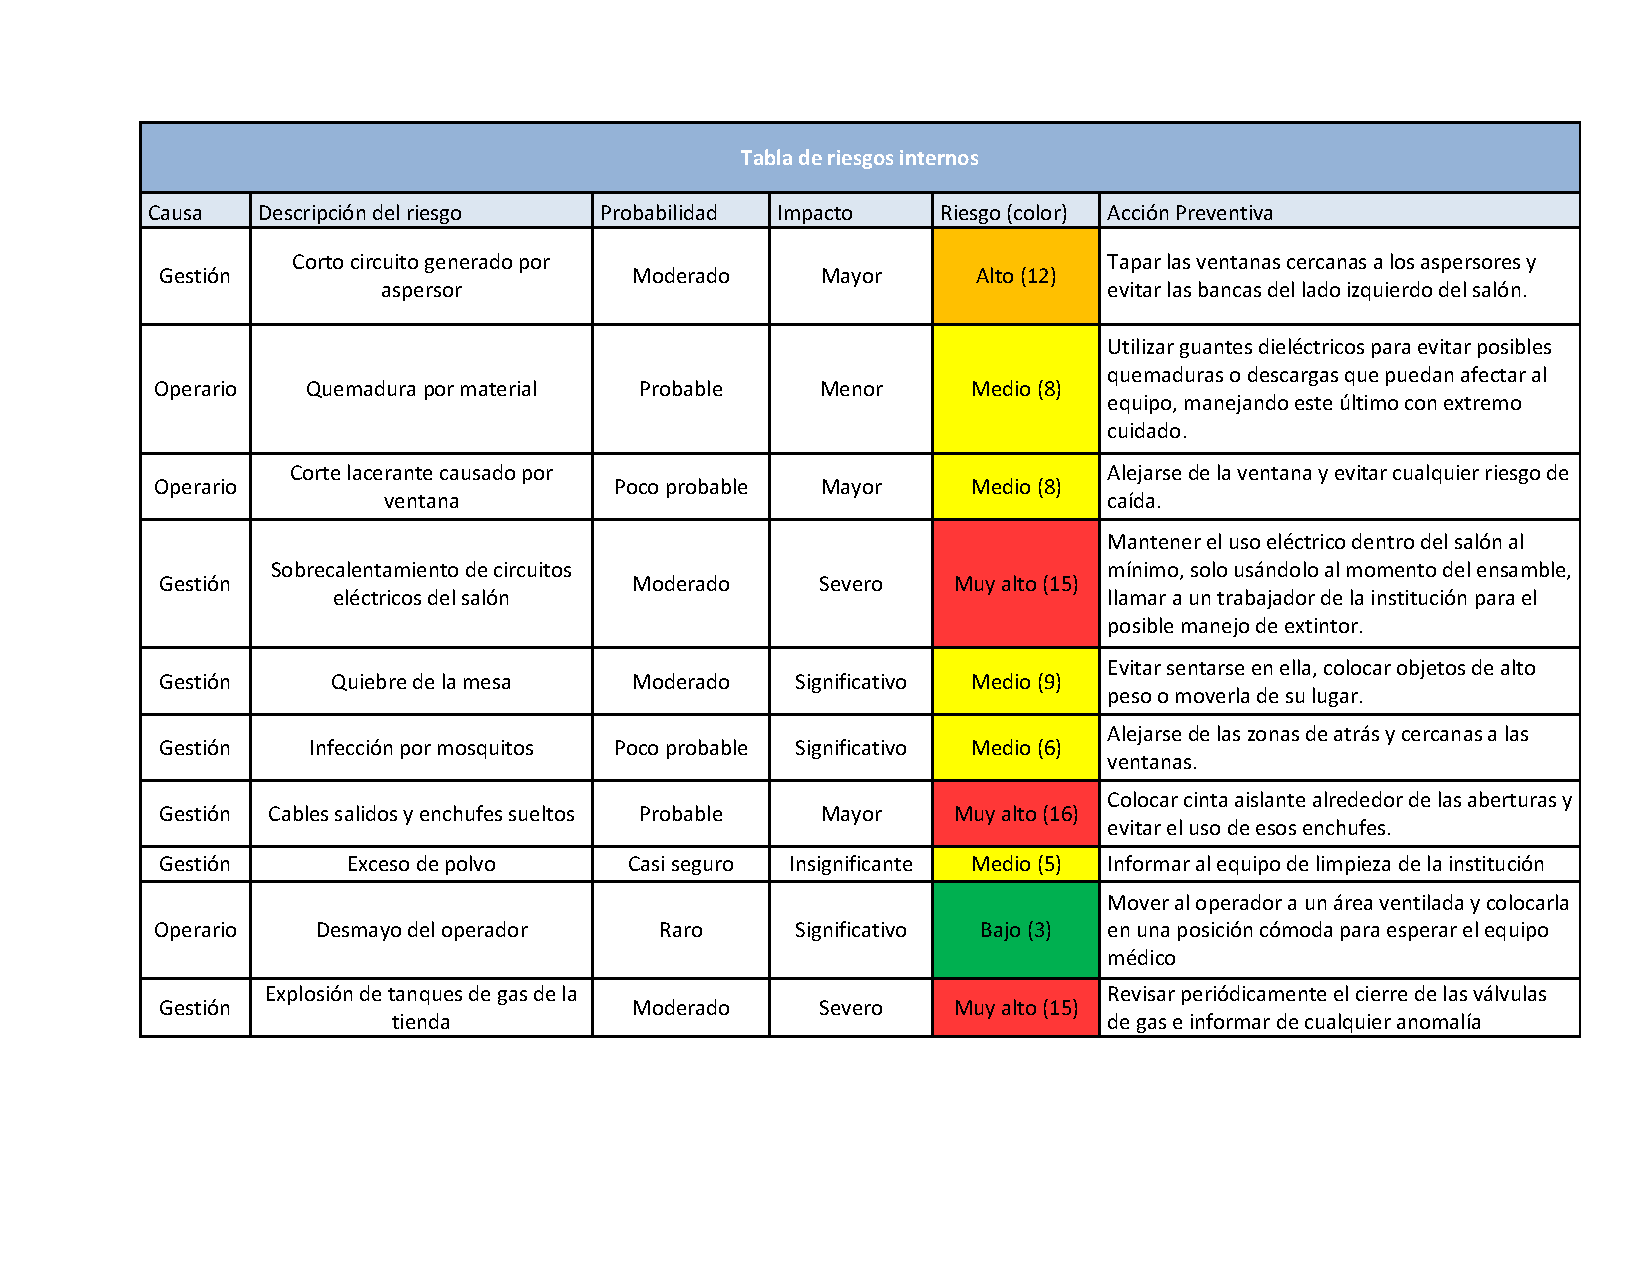
\includegraphics[trim = {20mm 15mm 10mm 20mm},clip,scale=0.35]{19/Img/riesgosInt.pdf}
        \caption{Tabla de riesgos internos que se pueden generar a la hora del ensamble en el edificio de salones C}
        \label{fig:riesgosInt}
    \end{figure}
    
    \subsubsection{Riesgos externos}

     Además de estos también existen los riesgos externos, los cuales a diferencia de los internos que ocurren a causa de algún factor dentro de la institución estos se generan por factores externos y que en casi todos los casos no tienen nada que ver con el Tecnológico, pero de igual manera pueden llegar a generar problemas para los alumnos y trabajadores dentro de las instalaciones de la institución, por lo que se debe de también poseer una tabla, la cual se presenta en la figura \ref{fig:riesgosExt}, la cual refleja el riesgo que este posee y un plan de acción para evitar que estos riesgos afecten el trabajo realizado .

     \begin{figure}[H]
        \centering
        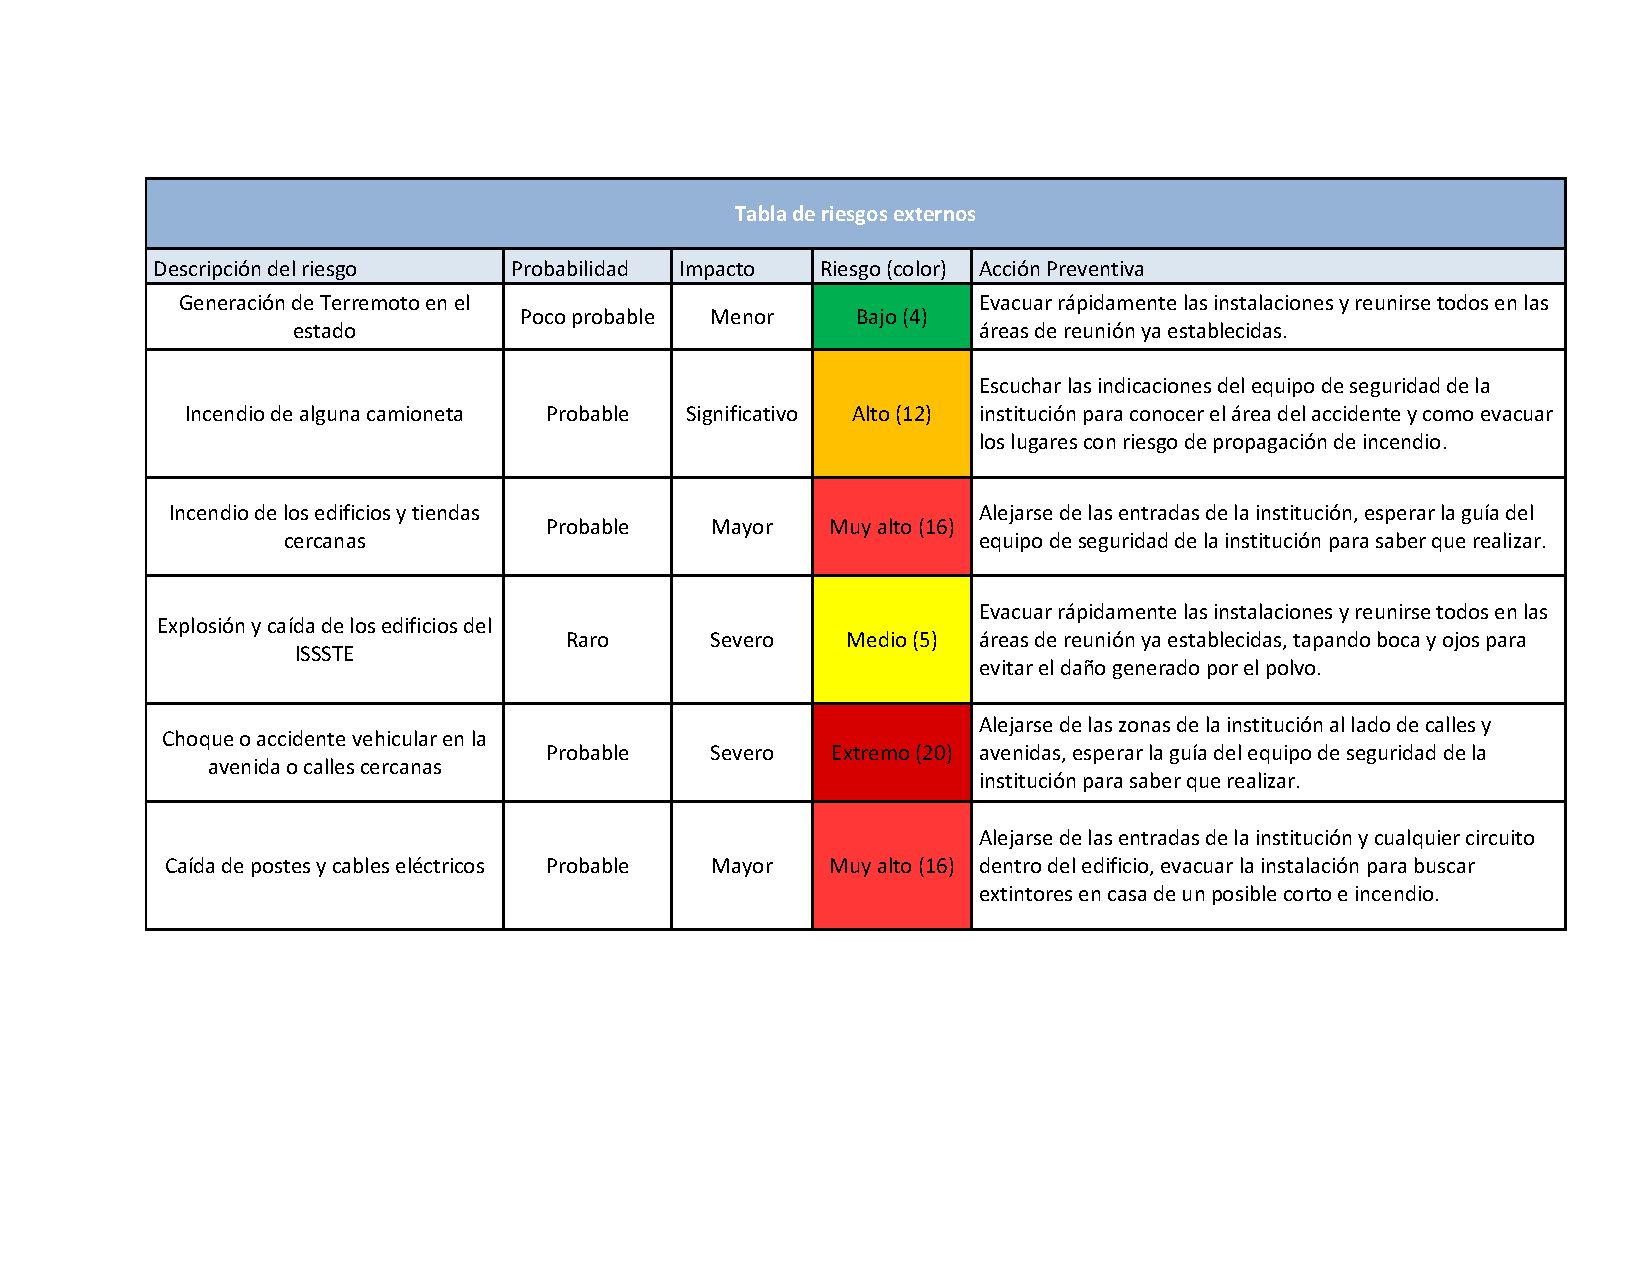
\includegraphics[trim = {20mm 80mm 10mm 20mm},clip,scale=0.35]{19/Img/riesgosExt.pdf}
        \caption{Tabla de riesgos internos que se pueden generar a la hora del ensamble en el edificio de salones C}
        \label{fig:riesgosExt}
    \end{figure}
     
    \subsubsection{Programa de actividades de prevención y auxilio}

Al ofrecer un servicio público es esencial que el Instituto Tecnológico ofrezca medidas de prevención en caso de que se generé algún fenómeno o evento extraordinario que pueda llegar a afectar la salud tanto de alumnos como de los trabajadores dentro de la institución, por lo cual se nos han brindado la información base a considerar en relación a posibles riesgos y accidentes que pueden afectar a nuestra salud.
Durante cada semestre se realizan simulacros en los cuales se pide a los alumnos abandonar los edificios y reunirse en los puntos de reunión ofrecidos por la escuela, Señalándonos el lugar en medio del simulacro para entender el área que toca a cada edificio en la institución.
\\También se nos presento de antemano el área de atención médica, la cual se encuentra cerca de los edificios J y nos ofrecen tanto apoyo médico como psicológico.
 \\Lastimosamente al realizar un estudio de la sala médica y consultar información con el enfermero que se encontraba en labor en ese momento pudimos detectar una gran cantidad de falencias que posee en cuanto a los materiales requeridos y solicitados, mostrándonos como a pesar de esta ser una de las áreas con botiquín este posee lo mínimo para considerarse uno, teniendo solo analgésicos y antipiréticos básicos (como el paracetamol), el cual dicho por el obtuvo de otro lugar ajeno al Tecnológico y equipo de limpieza de heridas como gasas y vendas pero nada más, apenas siendo útil para heridas no graves como raspones o cortes leves, sumado a que el tanque de gas nunca ha sido rellenado y los extintores, los cuales  dicho por el paramédico tampoco están rellenados, por lo que exceptuando los extintores presentes en el centro de información y el área de laboratorios, donde los laboratorios de química, electrónica todos los demás edificios pueden no tener medidas de seguridad adecuadas

 \subsubsection{Plan de acción}

 En base tanto a los riesgos internos como externos presentados anteriormente se debe de realizar un plan de acción en el que se presente que se debe de realizar para evitar de que esto ocurra, que hacer si este riesgo ya ocurrió y observar los resultados de llevar acabo estas acciones.

 \begin{figure}[H]
        \centering
        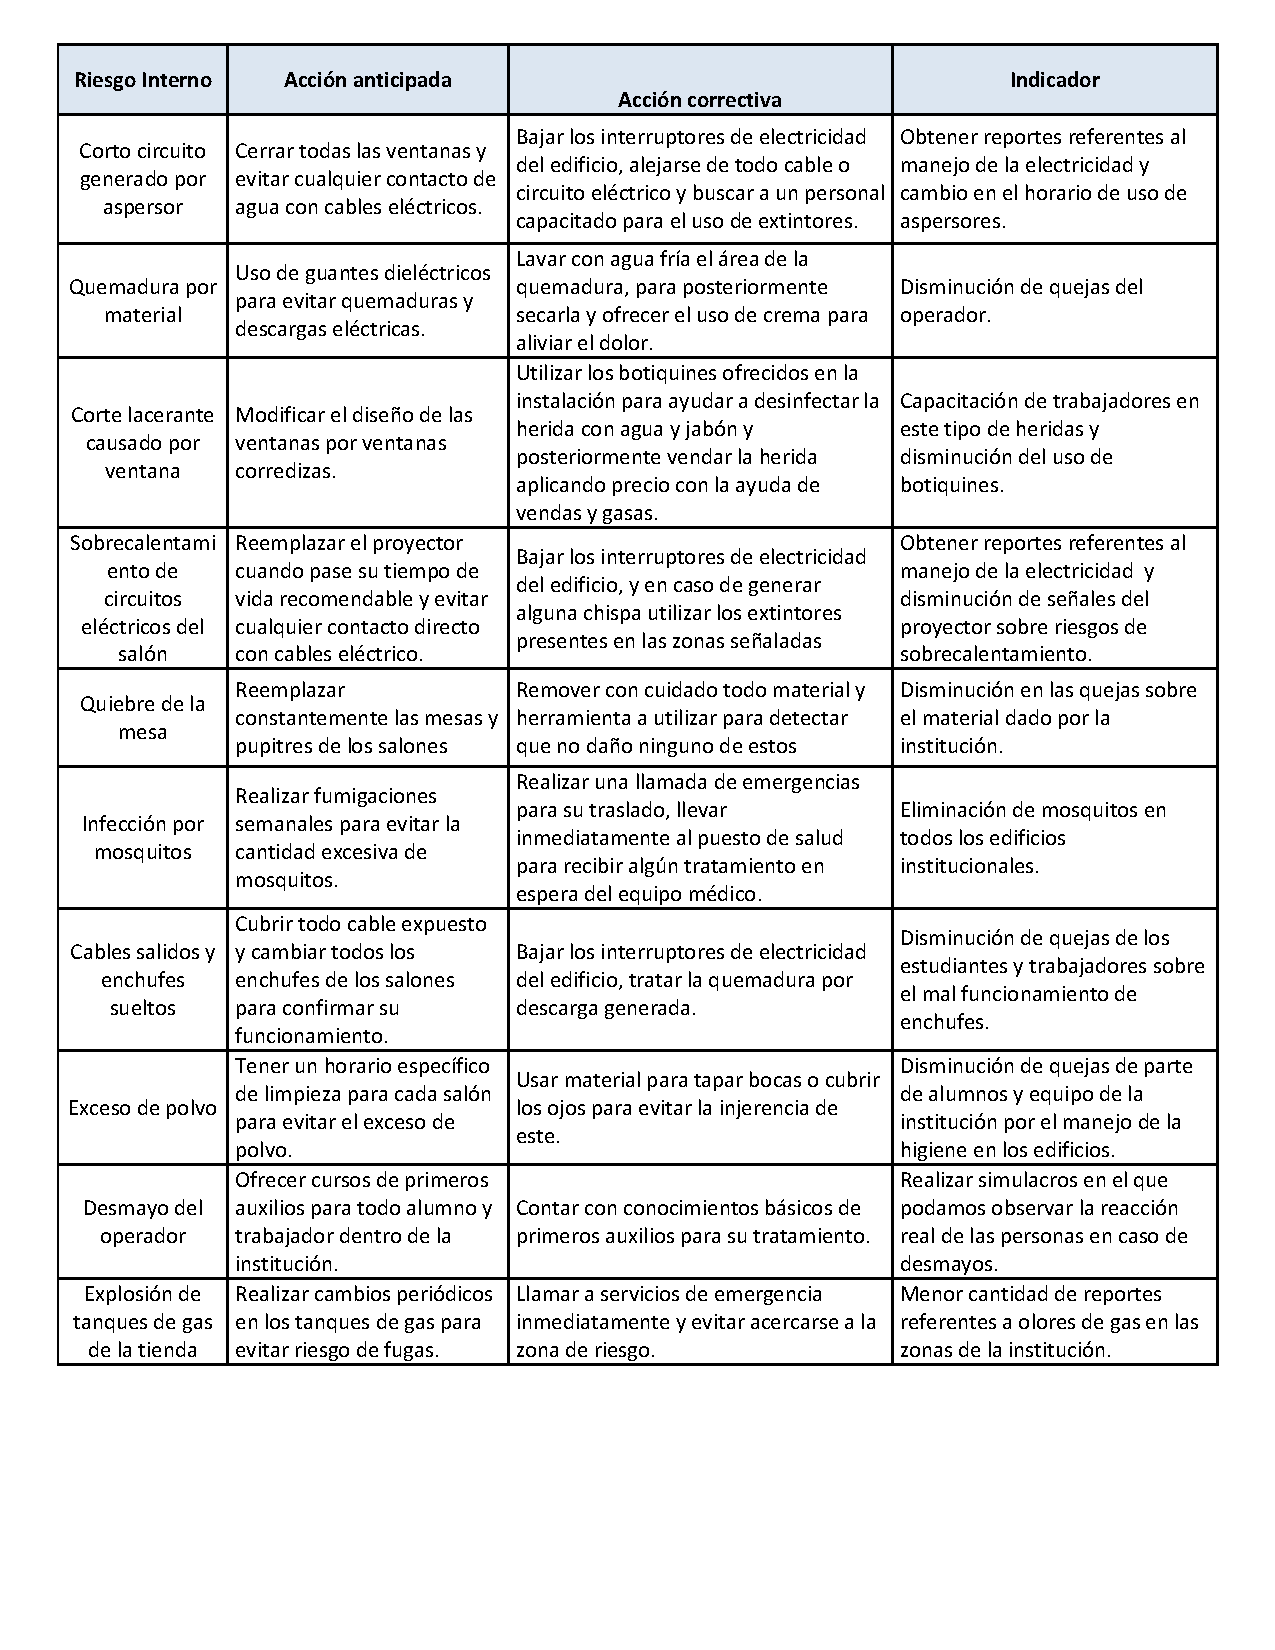
\includegraphics[trim = {1mm 40mm 1mm 1mm},clip,scale=0.35]{19/Img/accionAnti.pdf}
        \caption{Tabla de riesgos internos que se pueden generar a la hora del ensamble en el edificio de salones C}
        \label{fig:accionAnti}
    \end{figure}

    \begin{figure}[H]
        \centering
        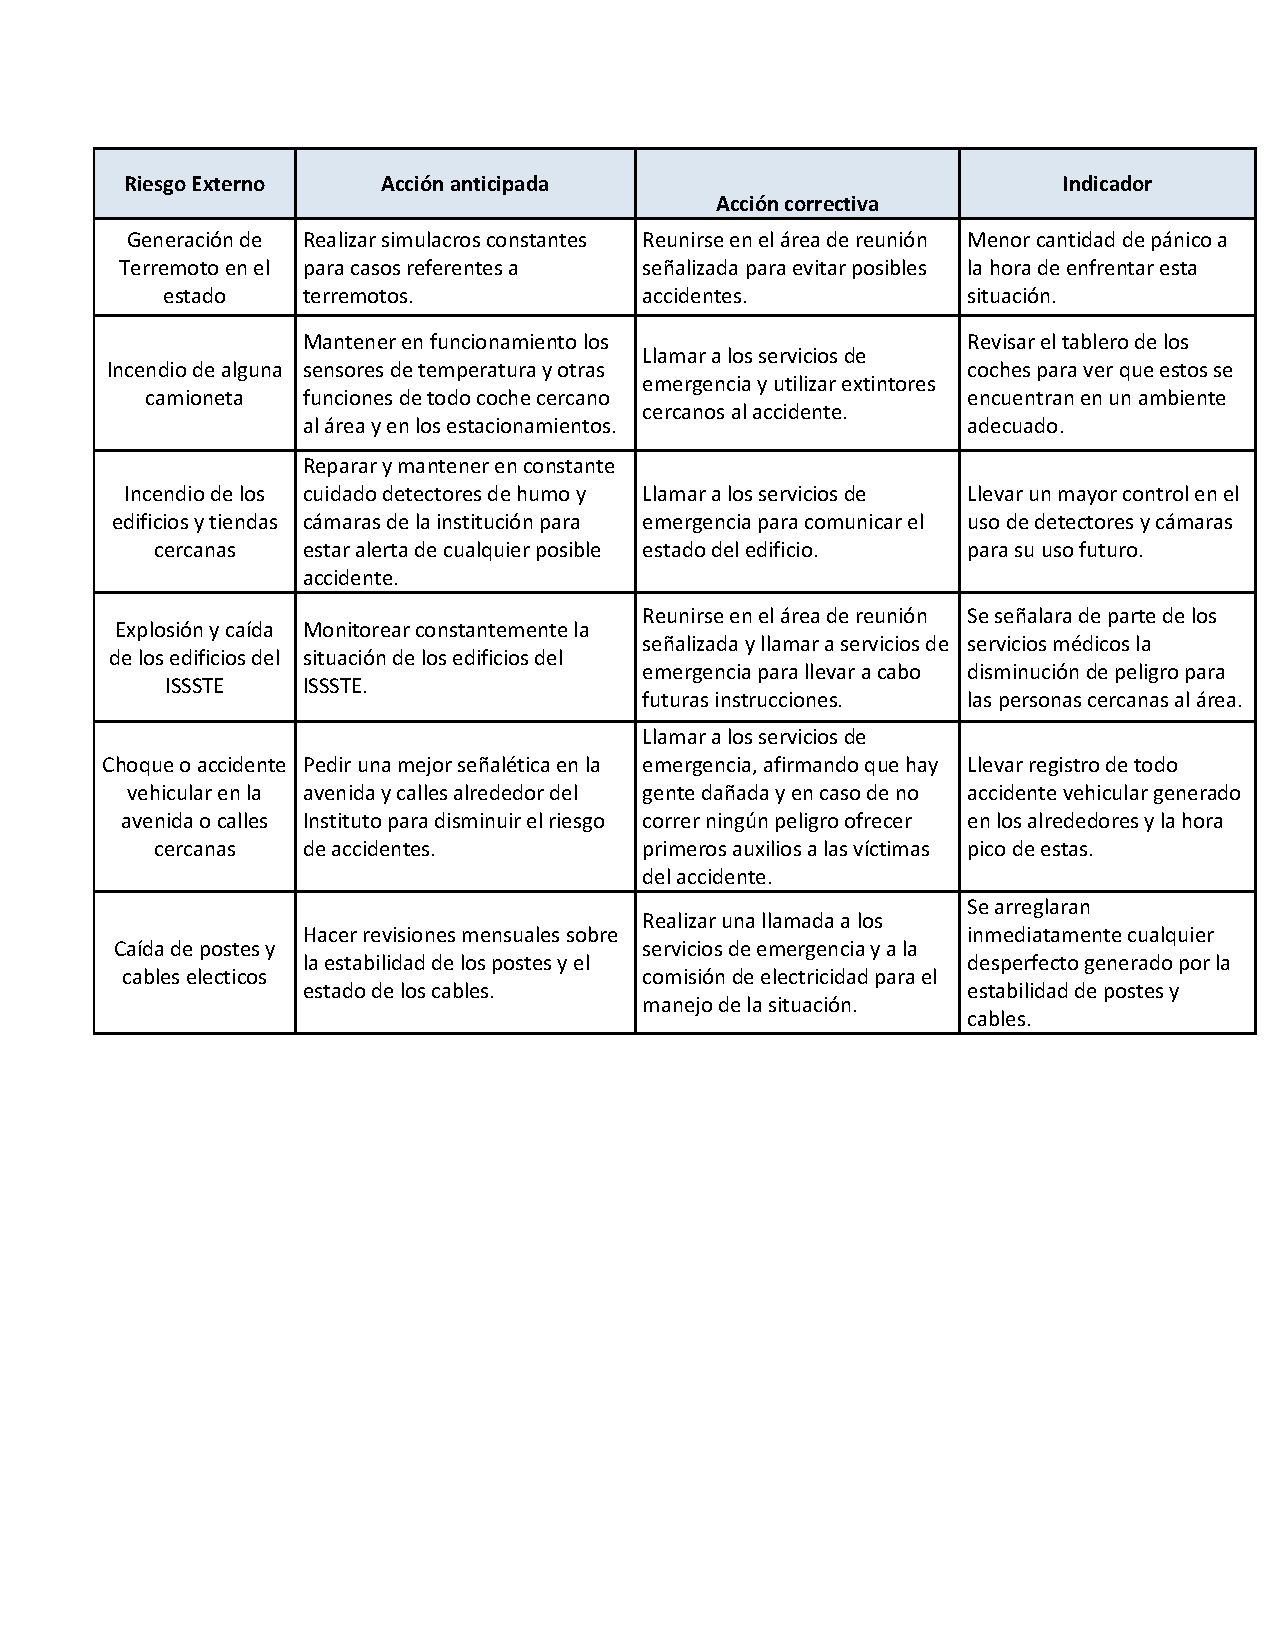
\includegraphics[trim = {1mm 100mm 1mm 10mm},clip,scale=0.35]{19/Img/accionAntiExt.pdf}
        \caption{Tabla de riesgos internos que se pueden generar a la hora del ensamble en el edificio de salones C}
        \label{fig:accionAntiExt}
    \end{figure}
     
     \subsubsection{Identificación de capacidades}

Como mencione es esencial el conocimiento de todo material referente al cuidado de la persona, por lo que se debe mantener un registro de todo equipo cercano al edificio relacionado con garantizar el bienestar de la persona como se presenta en la tabla \ref{tab:inventario}.

\begin{table}[H]
    \centering
    \caption{Recursos en materia de seguridad}
    \begin{tabular}{c c c}
    \hline
    \multicolumn{3}{c}{Inventario de recursos en materia de seguridad}\\
    \hline
         No.& Recurso & Cantidad  \\
    \hline
         1& Extintor & 5  \\
    \hline
         2& Botiquín & 2  \\
    \hline
         3& Detector de humo &  0\\
    \hline
         4& Lampara de emergencia &  2\\
    \hline     
    \end{tabular}
    \label{tab:inventario}
\end{table}

Para el caso de los extintores como mencione anteriormente se encuentran extintores colgados en los edificios del centro de información o C.I.y los laboratorios de eléctrica y mecánica, sumado al que se encuentra en el área médica y el segundo extintor del centro de información el cual mide aproximadamente un metro y es transportable, para el caso de botiquines además del área médica solo hay un botiquín cercano y es el que se encuentra en el C.I., mientras que no existe ningún detector de humo ni lamparas de emergencia en el edifico de salones C ni en áreas cercanas para el caso del detector, pero para el caso de las lamparas estas se encuentran en los laboratorios, los cuales son usados en caso de apagones.

\subsubsection{Plano de localización de recursos}

\begin{figure}[H]
    \centering
    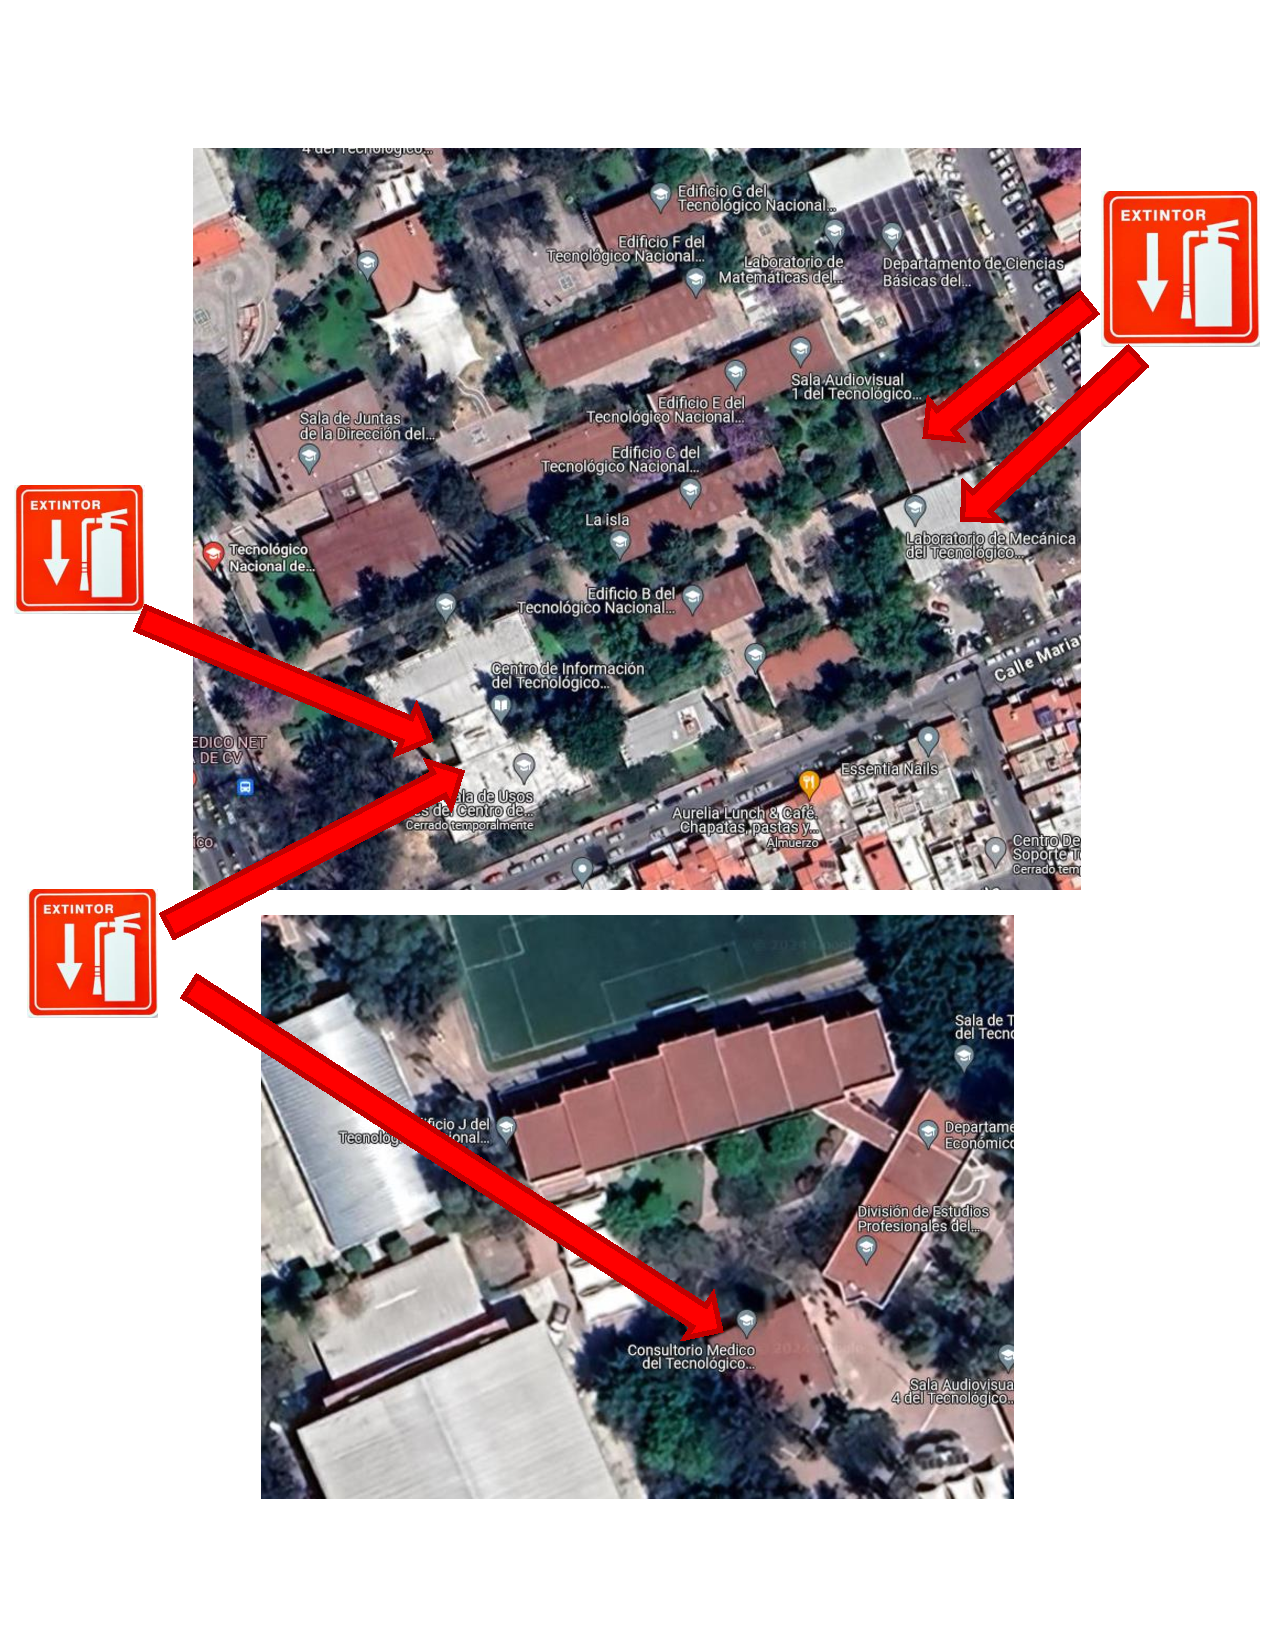
\includegraphics[trim = {0mm 25mm 0mm 12mm},clip,scale=0.3]{19/Img/planoLocalizadorExtintor.pdf}
    \caption{Plano del establecimiento de los Extintores en las cercanías del Edificio C.}
    \label{fig:planoLocalizadorExtintor}
\end{figure}
\begin{figure}[H]
    \centering
    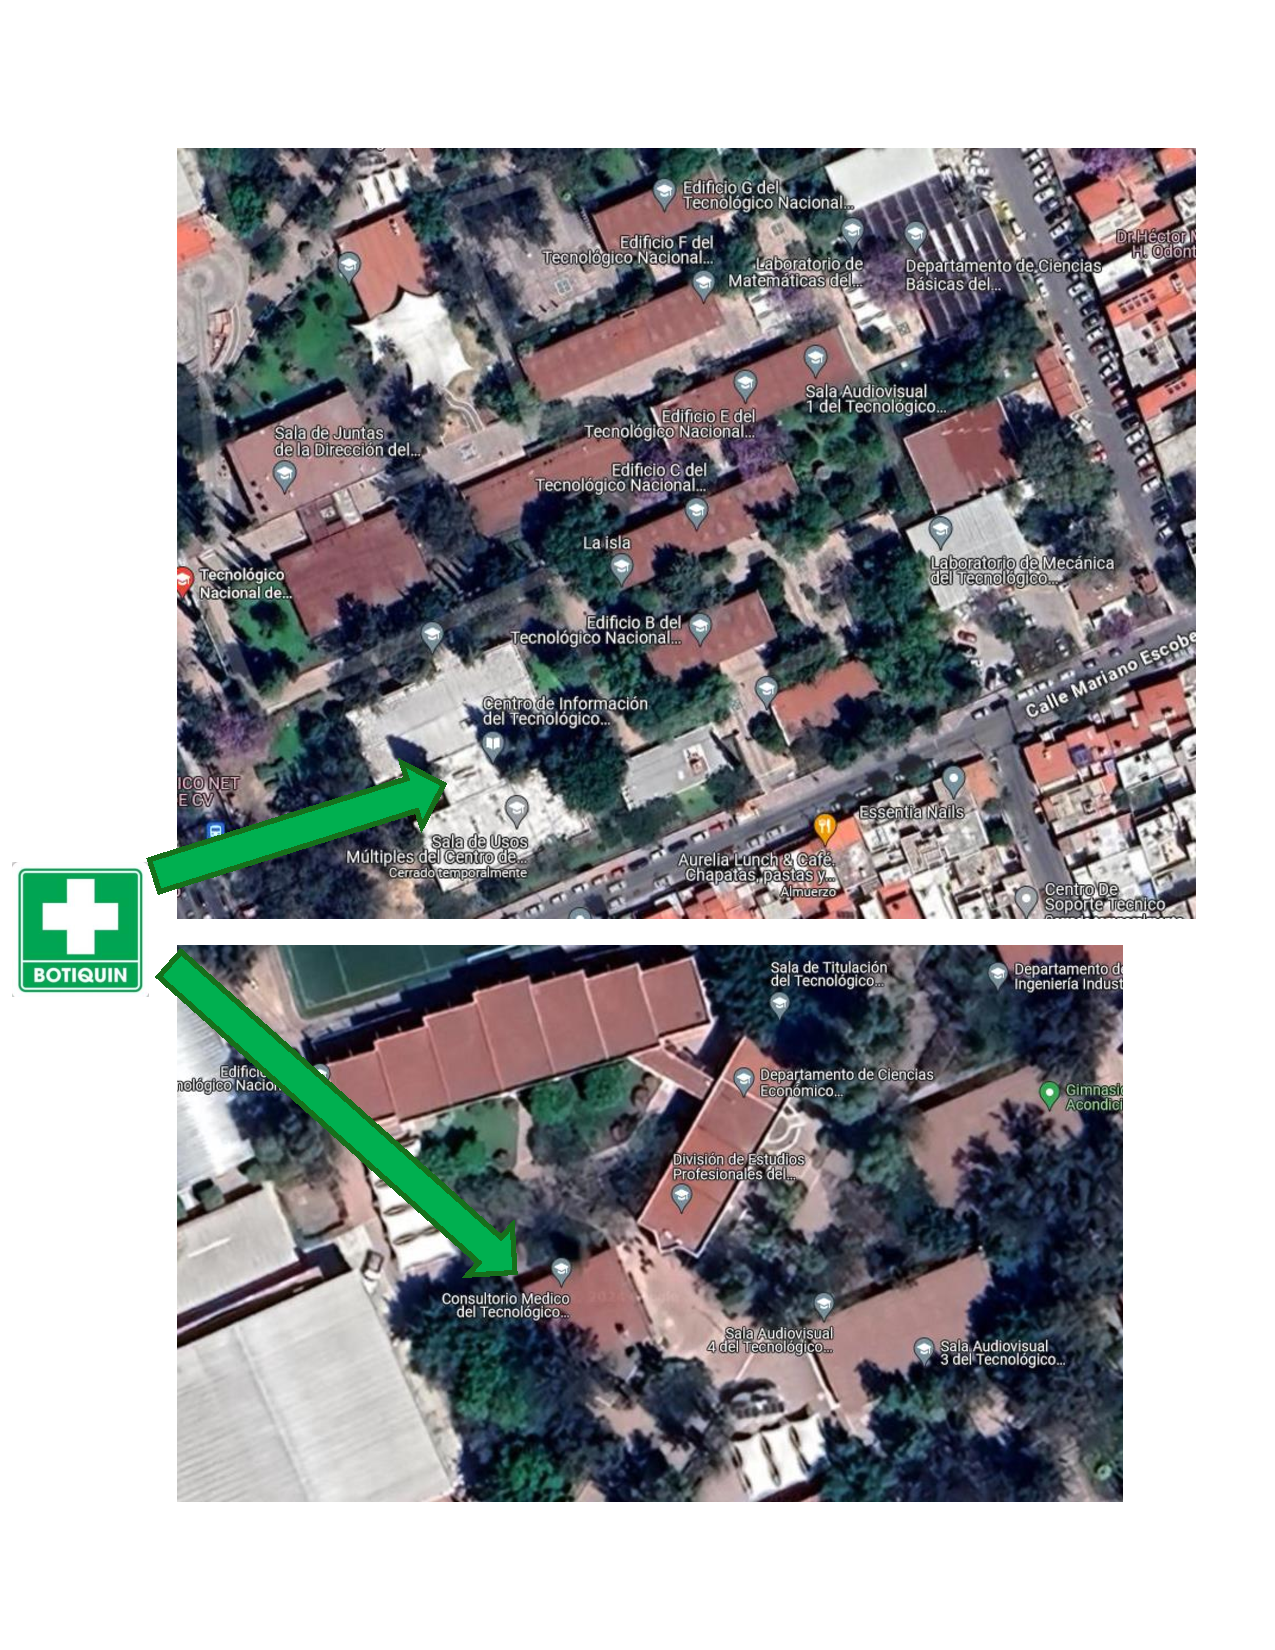
\includegraphics[trim = {0mm 25mm 0mm 12mm},clip,scale=0.3]{19/Img/planoLocalizadorBotiquin.pdf}
    \caption{Plano del establecimiento de los Botiquines en las cercanías del Edificio C.}
    \label{fig:planoLocalizadorBotiquin}
\end{figure}
\begin{figure}[H]
    \centering
    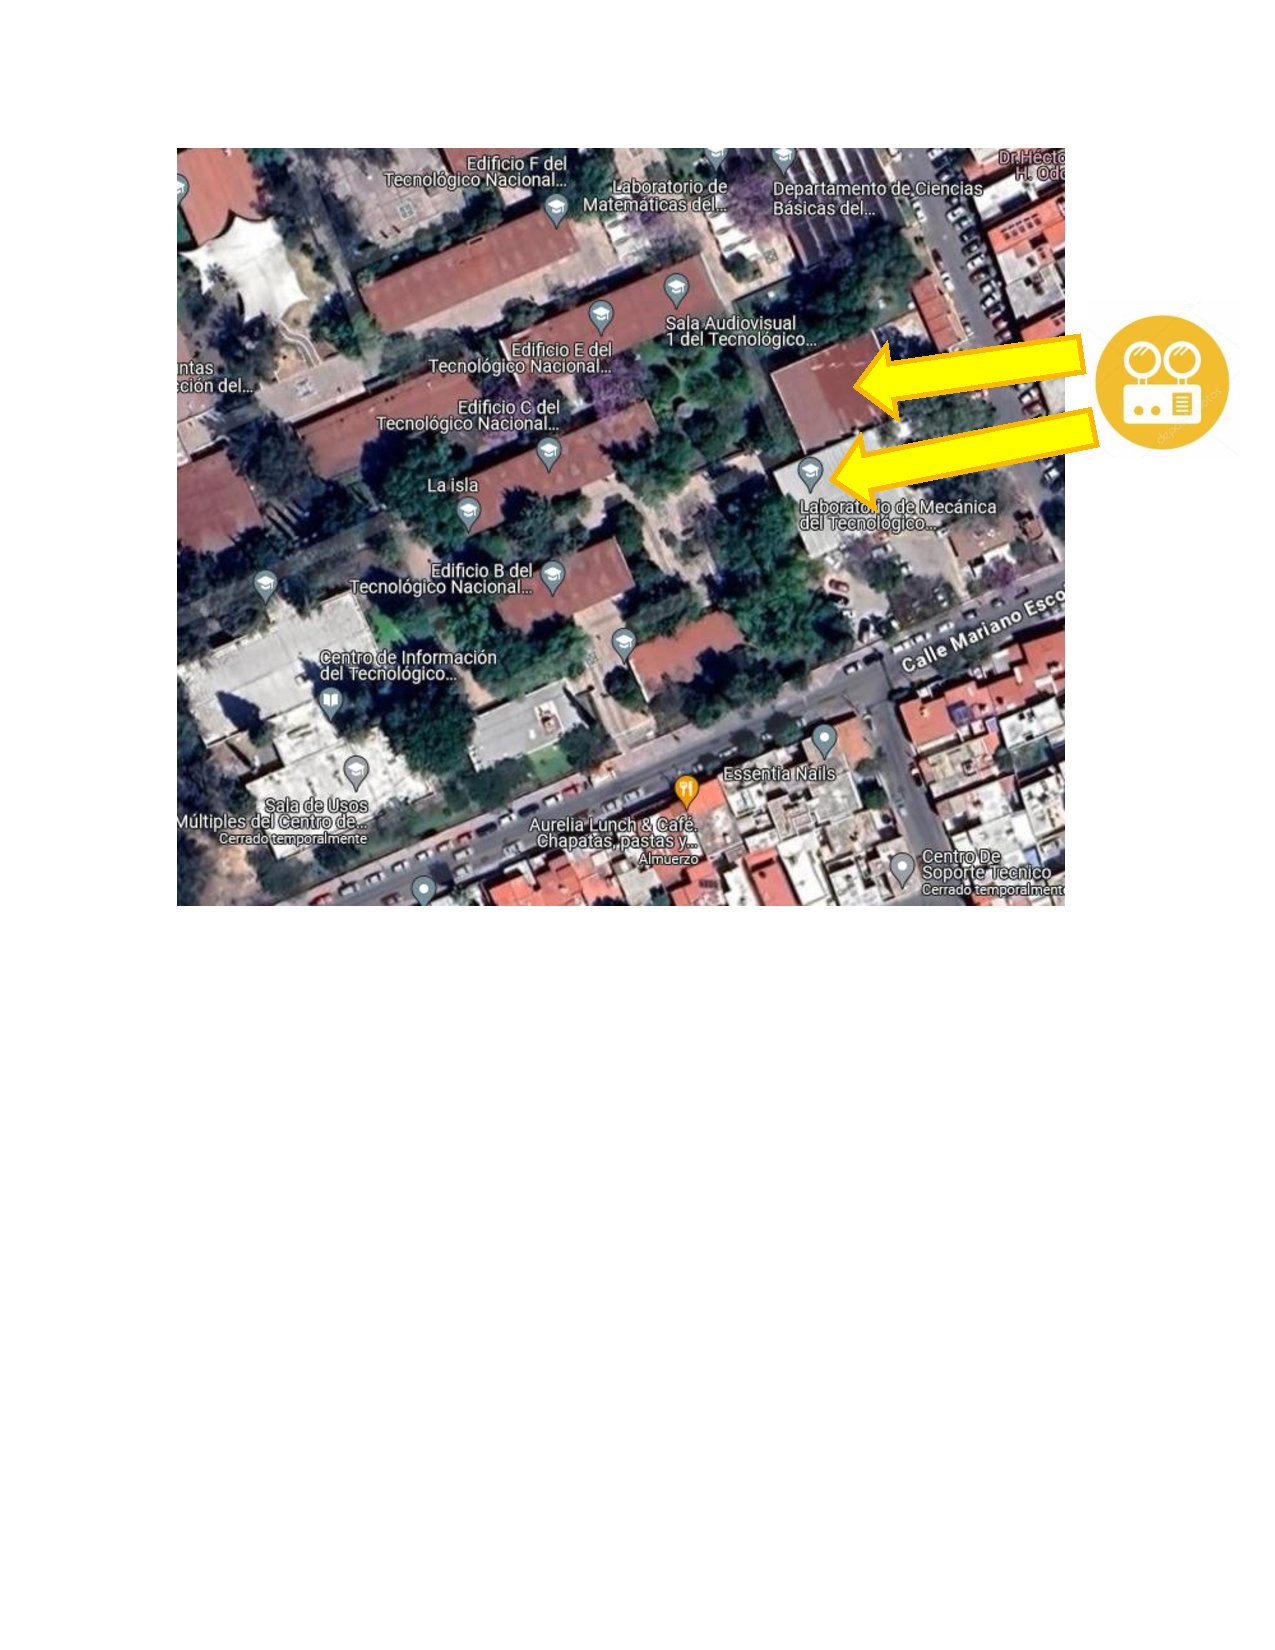
\includegraphics[trim = {0mm 140mm 0mm 12mm},clip,scale=0.3]{19/Img/planoLocalizadorLampara.pdf}
    \caption{Plano del establecimiento de las Lámparas de Emergencia en las cercanías del Edificio C.}
    \label{fig:planoLocalizadorLampara}
\end{figure}
\subsubsection{ Identificación de apoyos externos}
A pesar de todo esta sigue siendo una institución dedicada principalmente al desarrollo académico de futuros ingenieros por lo cual en muchos casos accidentes, enfermedades o diversas situaciones terminan rebasando la capacidad de los trabajadores por lo cual es pertinente poseer una lista de todo apoyo externo que exista en las cercanías de la institución, como se presenta en la figura \ref{fig:apoyosExt}.

\begin{figure}[H]
    \centering
    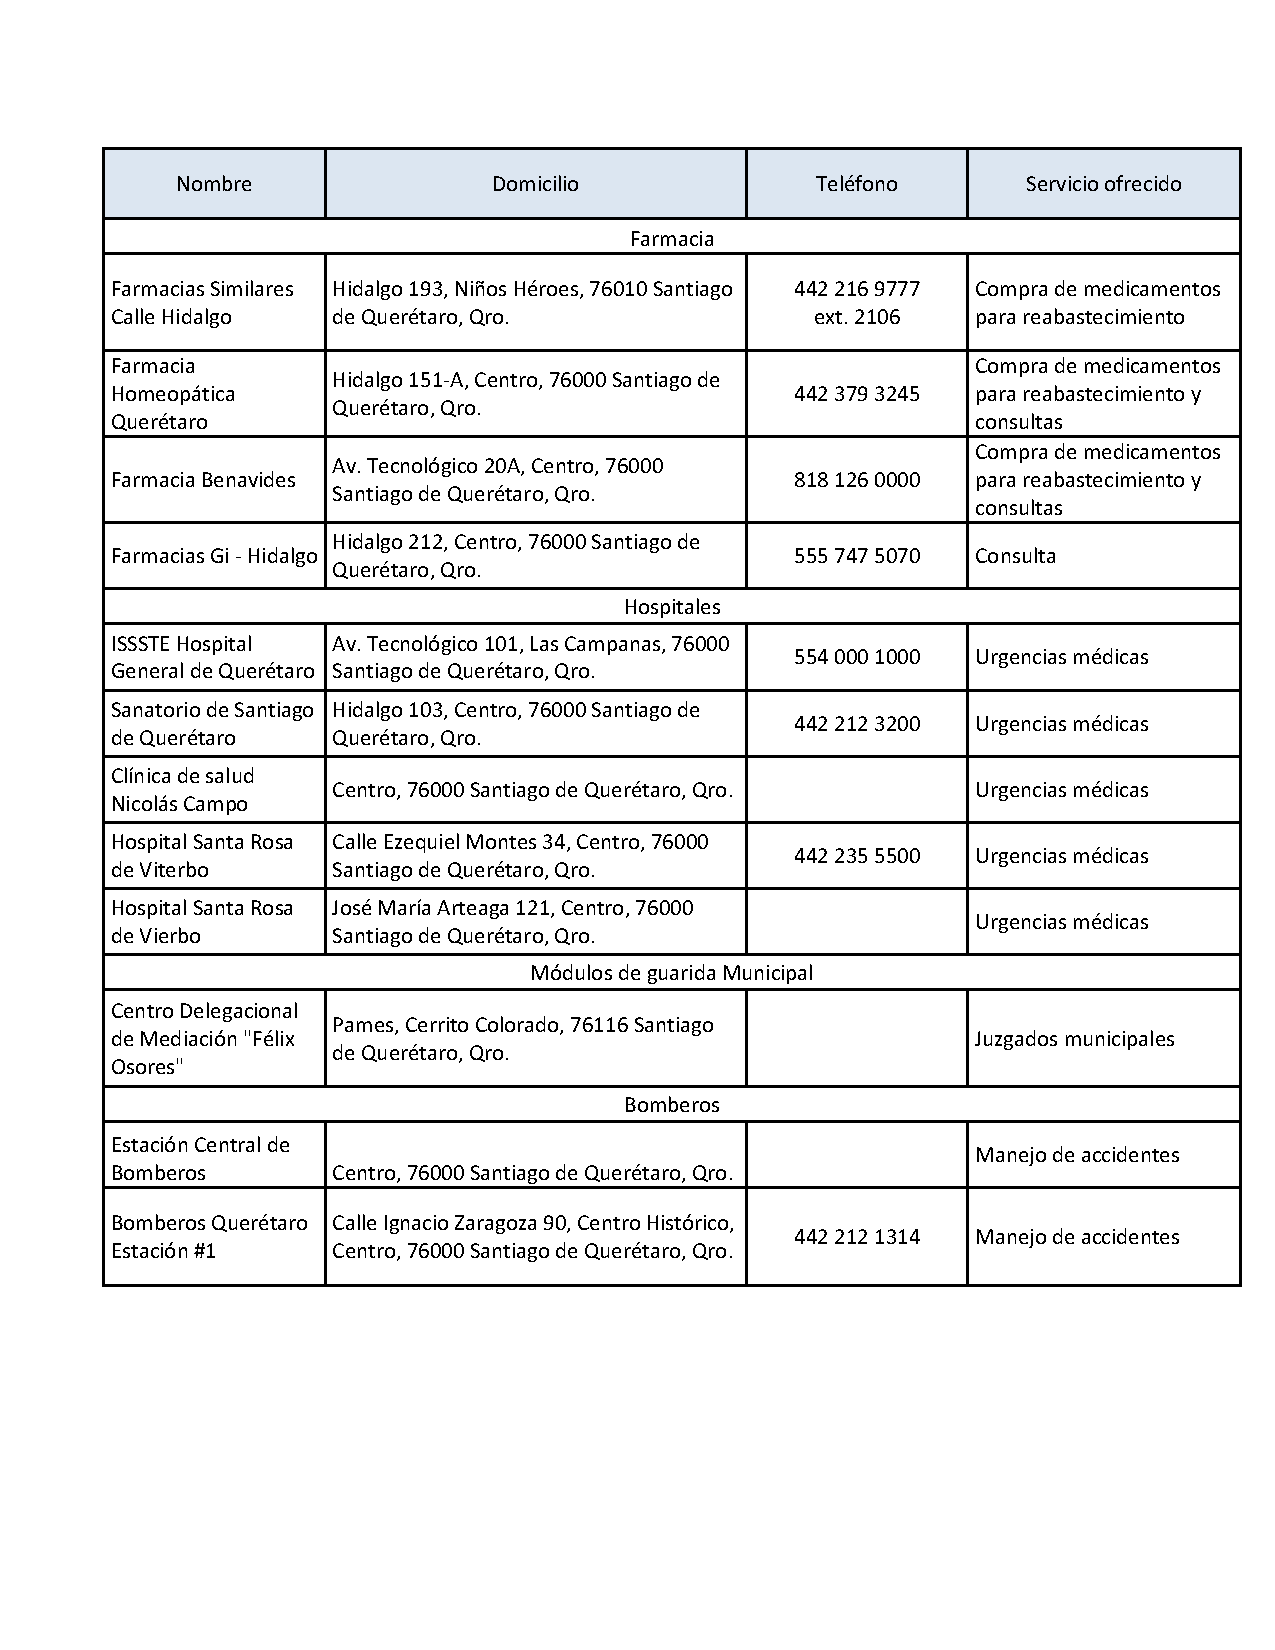
\includegraphics[trim = {15mm 60mm 5mm 25mm},clip,scale=0.4]{19/Img/apoyosExt.pdf}
    \caption{ Lugares que servirán de apoyo en un situación de emergencia.}
    \label{fig:apoyosExt}
\end{figure}
\subsubsection{Identificación de puntos de reunión}
Como se ha mencionado anteriormente uno de los lugares explicados a la hora de realizar un simulacro son los puntos de reunión, lugar donde se debe de resguardar para evitar cualquier daño generado por la caída o cualquier otro fenómeno que llegue a dañar la integridad de las estructuras circundantes, siendo en el caso del tecnológico debido a su gran tamaño se poseen diversas zonas de reunión en donde se deberán de reunir en base a los edificios y carreras circundantes.
\begin{figure}[H]
    \centering
    \includegraphics[trim = {100mm 140mm 20mm 40mm},clip,scale=0.6]{19/Img/puntosDeReunión.pdf}
    \caption{Zona segura en caso de una evacuación de emergencia.}
    \label{fig:puntosDeReunión}
\end{figure}
\subsubsection{Brigada de evacuación}

Al buscar información sobre una brigada relacionada a la institución o una autónoma generada por los trabajadores no había ninguna información de que esta existiera, sin embargo al momento de realizar los trabajos que una brigada debería tener se llego a la conclusión de que en caso de accidentes estas labores serian realizadas por los docentes que se encuentren en la zona en el momento del suceso.
\begin{figure}[H]
    \centering
    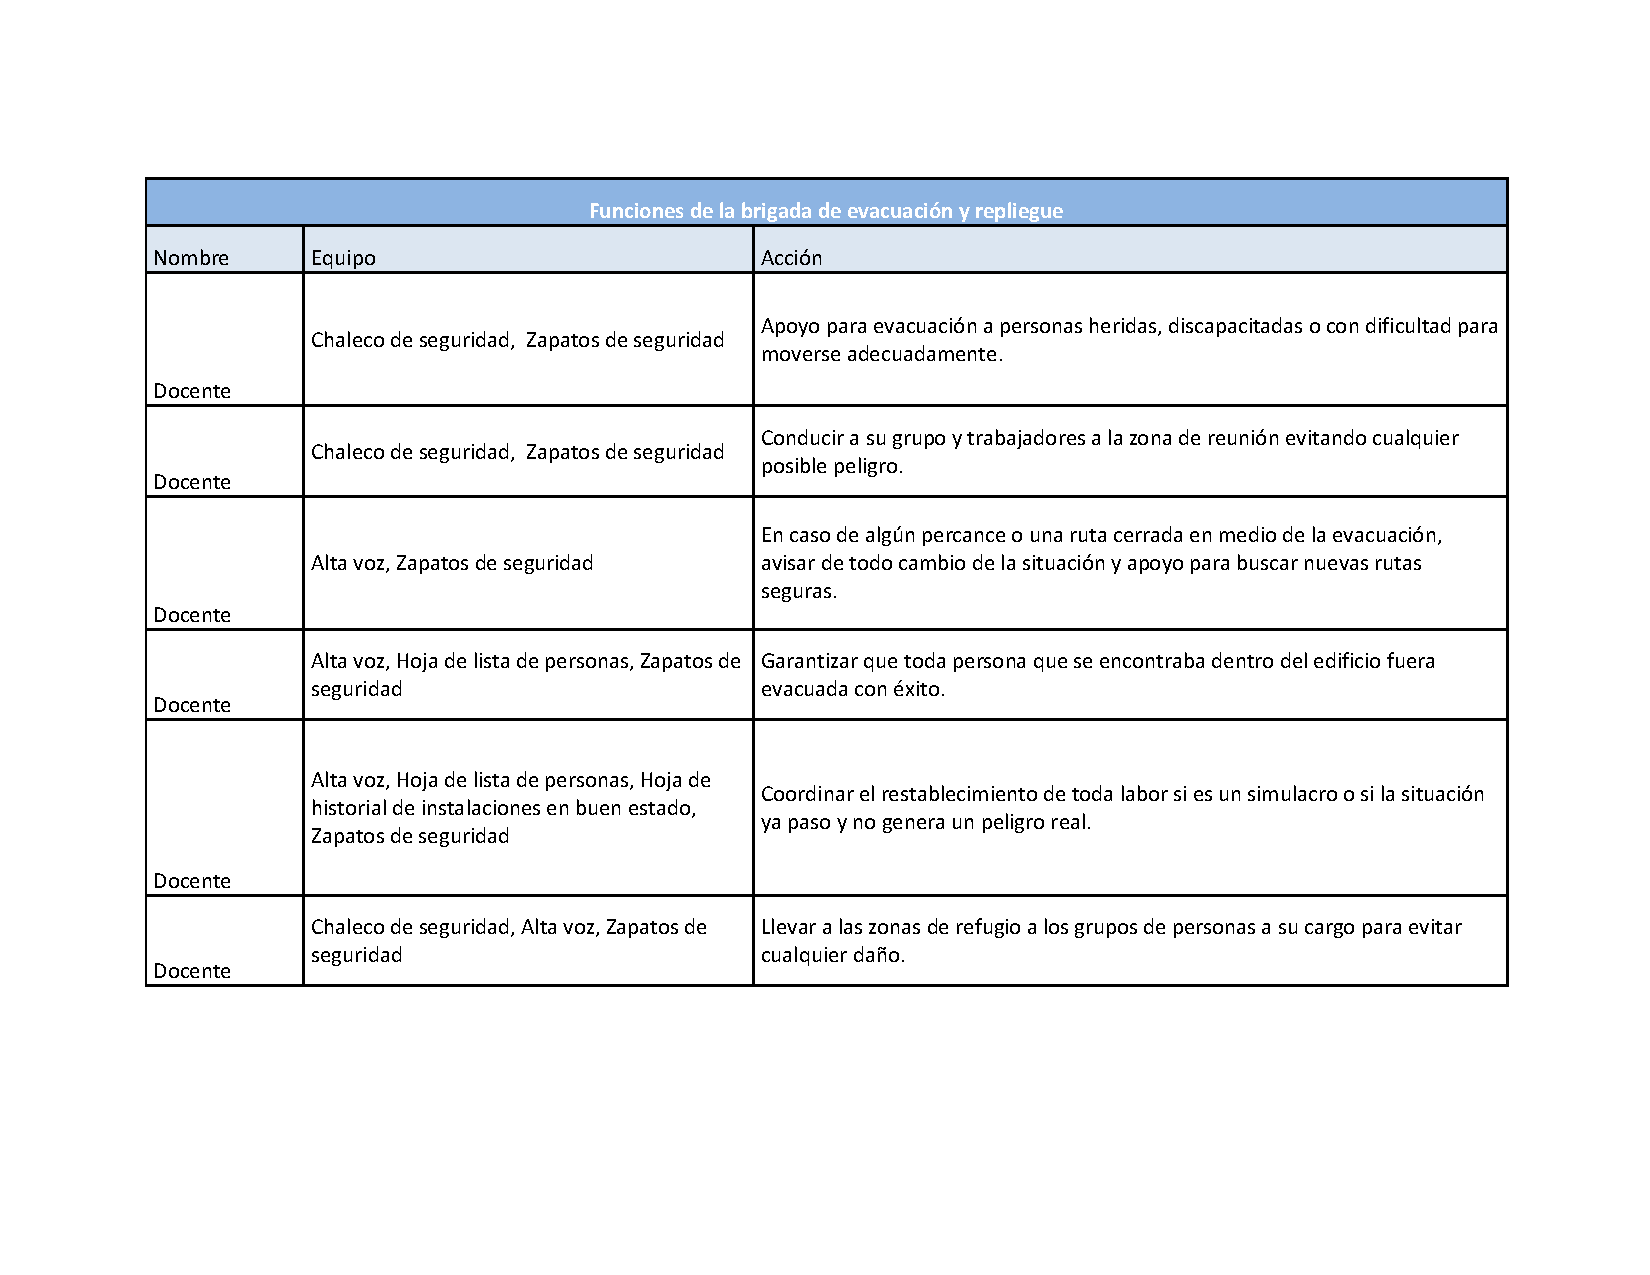
\includegraphics[trim = {20mm 40mm 20mm 10mm},clip,scale=0.35]{19/Img/brigadaEvacuacion.pdf}
    \caption{Acciones asignadas a realizar por el grupo de docentes para la Brigada de evacuación.}
    \label{fig:brigadaEvacuacion}
\end{figure}
\subsubsection{Directorio de telefónicos de emergencia}
En caso de algún accidente o situación en la que no puede ser manejada por el equipo interno de la institución y no se puede trasladar hacia algún hospital es necesario tener una lista con los numero primordiales a llamar en caso de cualquier percance, siendo primordialmente el mas común de todos \ref{fig:numero911}.
\begin{figure}[H]
    \centering
    
\includegraphics[trim = {20mm 30mm 20mm 30mm},clip,scale=0.35]{19/Img/numero911.pdf}
    \caption{Número de emergencias básico en México.}
    \label{fig:numero911}
\end{figure}

\begin{figure}[H]
    \centering
    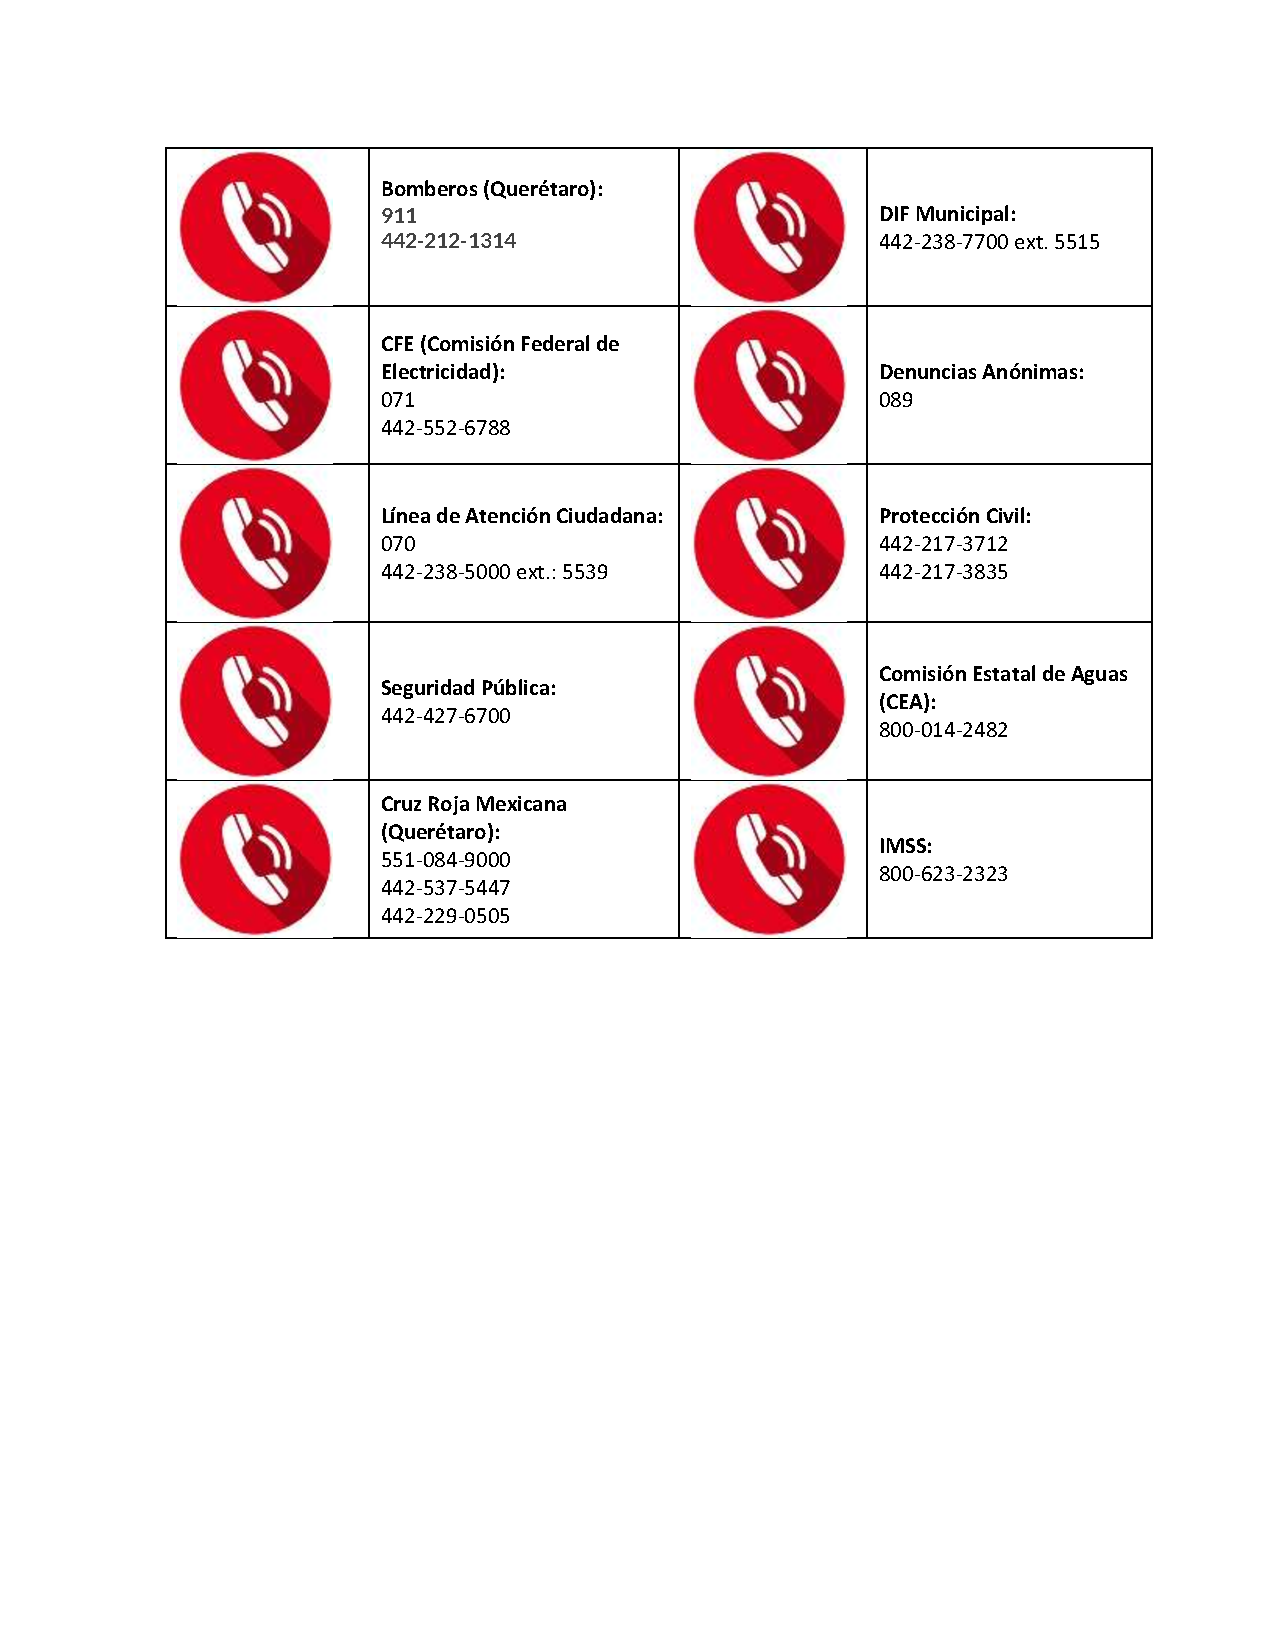
\includegraphics[trim = {25mm 120mm 20mm 20mm},clip,scale=0.5]{19/Img/directorioSeguridad.pdf}
    \caption{Directorio de todos los números necesarios en caso de algún accidente.}
    \label{fig:directorioSeguridad}
\end{figure}

     \subsection{Análisis de los métodos, materiales, herramientas e instalación utilizada en la ejecución del ensamble de un circuito electrónico}
\subsubsection{Verificación}
    
    Ya con la lectura, análisis y memorización del manual de fabricación por parte del operador se iniciara de manera manual el ensamblaje del circuito a manos del operador, rellenando una hoja de referencia con todos los datos solicitados para poder llevar acabo la operación \ref{fig:tablaOperador}, mientras que el analista observa y realice la película (muestra continua) sobre como el operario llevo acabo todo el proceso de ensamblaje utilizando únicamente como base las instrucciones dadas con anterioridad, sin ningún tipo de apoyo externo, para de esta manera concluir si el circuito fue armado correctamente.
\begin{figure}[H]
    \centering
    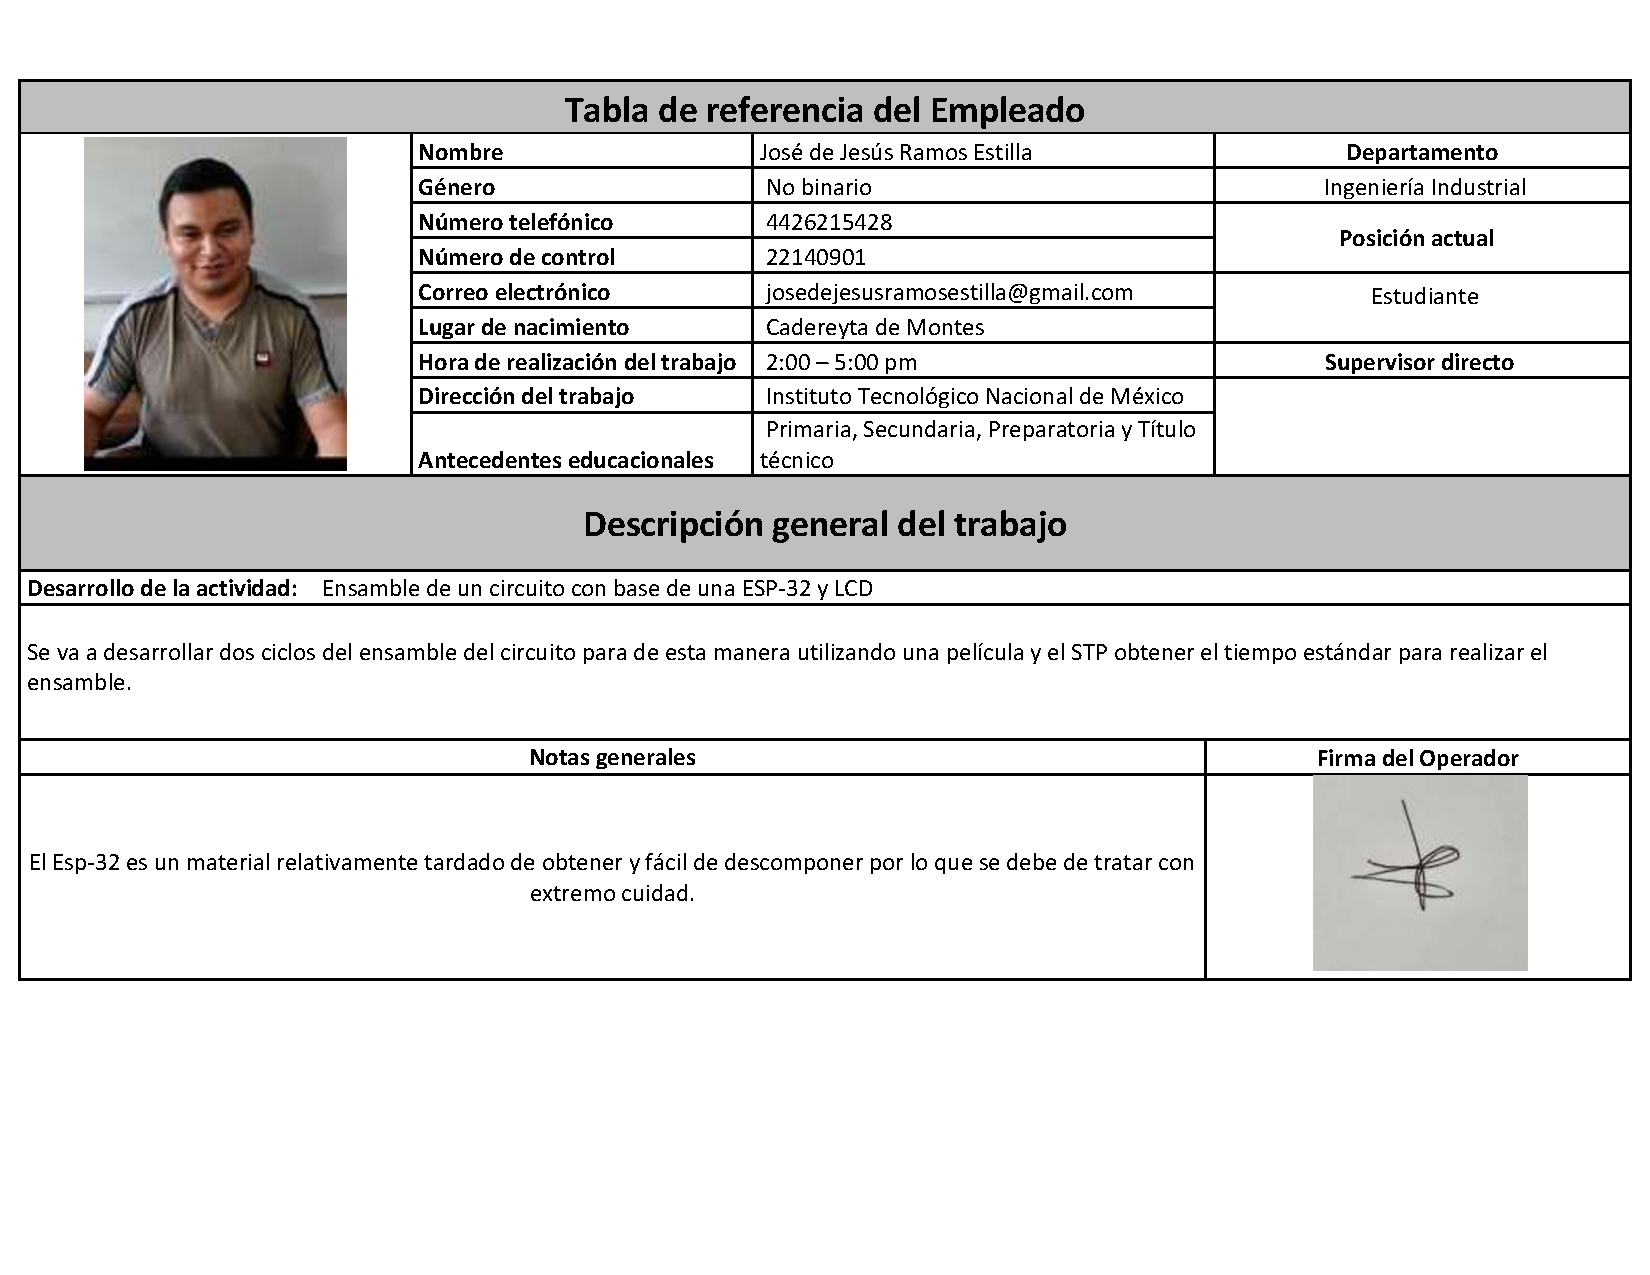
\includegraphics[trim = {1mm 50mm 1mm 1mm},clip,scale=0.3]{19/Img/tablaOperador.pdf}
    \caption{Hoja de referencia del Operador José de Jesús Ramos.}
    \label{fig:tablaOperador}
\end{figure}
    Al terminar todo el proceso de armado para confirmar que este se realizo adecuadamente se necesitará que el operador realice una modificación al rango del potenciómetro, al moverlo y modificar su resistencia para observar su cambio en la pantalla, de esta manera el analista deberá de tomar evidencia de como no solo la pantalla LCD funciona adecuadamente al prender y enviar una señal, sino también el hecho de que si se genera algún cambio en la lectura ofrecida por el potenciómetro a la hora de variar la resistencia de este último como se y de esta manera poder verificar que estos cambios ocurren de manera adecuada como en la figura \ref{fig:evidenciaCambio1}.
                \begin{figure}[H]
        \centering
        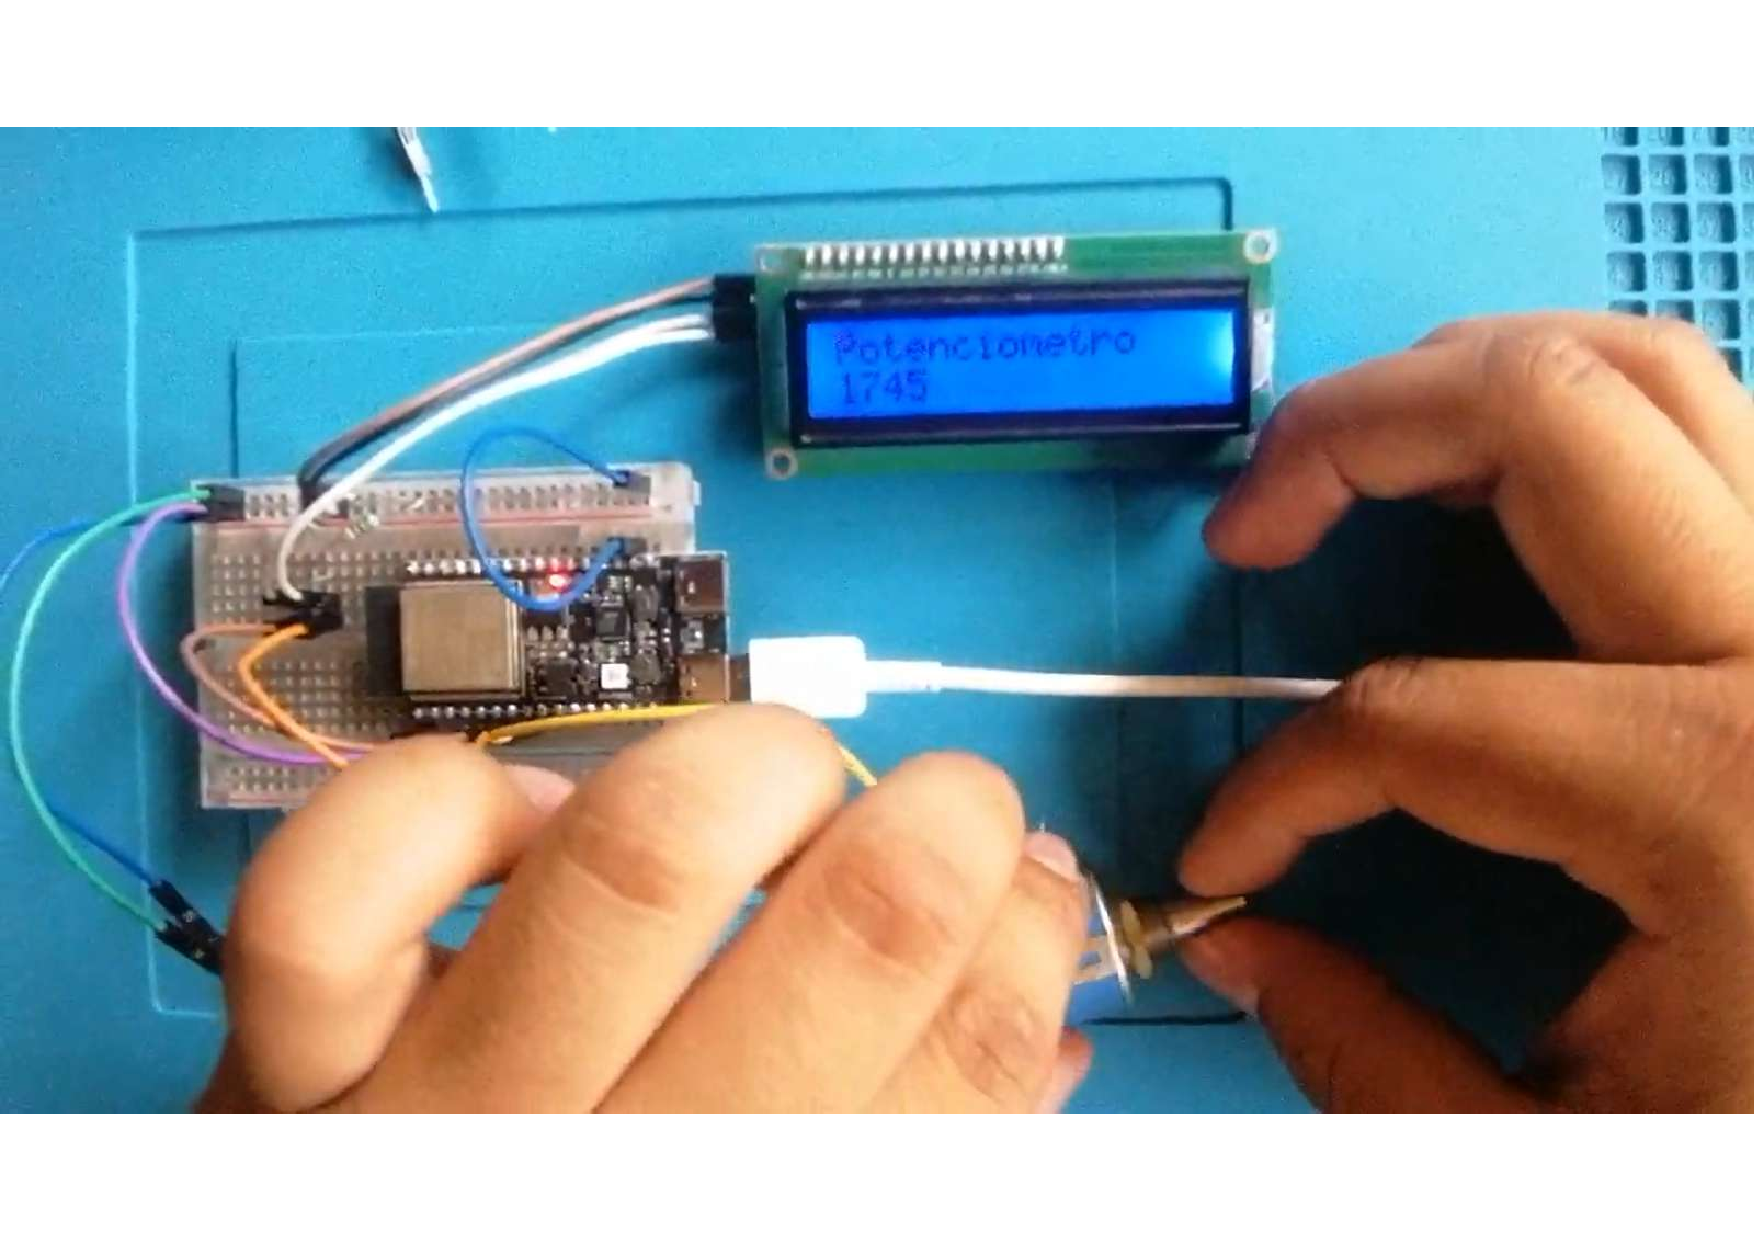
\includegraphics[trim = {50mm 20mm 0mm 0mm},clip,scale=0.3]{19/Img/evidenciaCambio1.pdf}
        \caption{Primer lectura obtenida a la hora de armar el circuito por primera vez.}
        \label{fig:evidenciaCambio1}
    \end{figure}
    Como se puede observar en la figura \ref{fig:evidenciaCambio1} se puede confirmar como al realizar el ensamble usando como base el manual realizado se logro no solo que se generará una señal a la pantalla, sino además como se muestra en la figura \ref{fig:evidenciaCambio2} se puede confirmar que a la hora de mover el potenciómetro este efectivamente cambio el valor presentado en el LCD, por lo que puede pasar la prueba de verificación.
                    \begin{figure}[H]
        \centering
        \includegraphics[trim = {50mm 20mm 0mm 0mm},clip,scale=0.3]{19/Img/evidenciaCambio2.pdf}
        \caption{Segunda lectura obtenida a la hora de armar el circuito por primera vez.}
        \label{fig:evidenciaCambio2}
    \end{figure}
    Continuando con el mismo proceso se realizaron otras dos modificaciones al valor de la resistencia del potenciómetro para de esta manera tener evidencia sólida de que la modificación y todo el proceso fue el adecuado, demostrado en las siguientes figuras:
    \begin{figure}[H]
        \centering
        \includegraphics[trim = {50mm 20mm 0mm 0mm},clip,scale=0.3]{19/Img/evidenciaCambio3.pdf}
        \caption{Tercera lectura obtenida a la hora de armar el circuito por primera vez.}
        \label{fig:evidenciaCambio3}
    \end{figure}
\begin{figure}[H]
        \centering
        \includegraphics[trim = {50mm 20mm 0mm 0mm},clip,scale=0.3]{19/Img/evidenciaCambio4.pdf}
        \caption{Cuarta lectura obtenida a la hora de armar el circuito por primera vez.}
        \label{fig:evidenciaCambio4}
    \end{figure}

    Como se muestra en las figuras \ref{fig:evidenciaCambio3} y \ref{fig:evidenciaCambio4}, podemos confirmar que los cuatro cambios requeridos para la verificación del primer ciclo por lo que aceptamos que el ensamble del circuito se realizo de manera exitosa, por lo que se deberá de realizar el mismo procedimiento en otro día para poder obtener los valores de tiempo de otro ciclo del mismo operador.
    \\Después de realizado todo el ensamble al día siguiente pudimos observar una disminución en la iluminación del LCD, sin embargo gracias a la figura \ref{fig:evidenciaCambio5} podemos observar que si da señal y si genera una lectura del potenciómetro, por lo que para confirmar el cambio en la resistencia de este al igual que el día anterior se movió el valor del potenciómetro para observar el cambio, pudiendo observar un cambio en las otras lecturas de las figuras \ref{fig:evidenciaCambio6}, \ref{fig:evidenciaCambio7} y \ref{fig:evidenciaCambio8} por lo que al igual que le ciclo anterior este se concluyo satisfactoriamente.

\begin{figure}[H]
        \centering
        \includegraphics[trim = {50mm 20mm 0mm 5mm},clip,scale=0.3]{19/Img/evidenciaCambio5.pdf}
        \caption{Primera lectura obtenida a la hora de armar el circuito por segunda vez.}
        \label{fig:evidenciaCambio5}
    \end{figure}
    \begin{figure}[H]
        \centering
        \includegraphics[trim = {50mm 20mm 0mm 10mm},clip,scale=0.3]{19/Img/evidenciaCambio6.pdf}
        \caption{Segunda lectura obtenida a la hora de armar el circuito por segunda vez.}
        \label{fig:evidenciaCambio6}
    \end{figure}
    \begin{figure}[H]
        \centering
        \includegraphics[trim = {50mm 20mm 0mm 0mm},clip,scale=0.3]{19/Img/evidenciaCambio7.pdf}
        \caption{Tercera lectura obtenida a la hora de armar el circuito por segunda vez.}
        \label{fig:evidenciaCambio7}
    \end{figure}
    \begin{figure}[H]
        \centering
        \includegraphics[trim = {50mm 20mm 0mm 0mm},clip,scale=0.3]{19/Img/evidenciaCambio8.pdf}
        \caption{Cuarta lectura obtenida a la hora de armar el circuito por segunda vez.}
        \label{fig:evidenciaCambio8}
    \end{figure}

    \subsubsection{Desarrollo del sistema de tiempos predeterminado}

    Después de confirmar que ambos ciclos se realizaron de manera exitosa se debe de utilizar un diagrama Bimanual que permitirá al analista poder observar los movimientos llevados acabo por el operador a la hora de armar el circuito, colocando el tapete como base se hará una separación de acciones en el que se especificara que movimientos se utilizaran para cada mano.

    \begin{figure}[H]
        \centering
        \includegraphics[trim = {280mm 1318mm 250mm 0mm},clip,scale=0.25]{19/Img/diagramaBimanual1.pdf}
        \newpage
        \label{fig:diagramaBimanual11}
    \end{figure}
\begin{figure}[H]
        \centering
        \includegraphics[trim = {280mm 500mm 250mm 790mm},clip,scale=0.25]{19/Img/diagramaBimanual1.pdf}
        \newpage
        \label{fig:diagramaBimanual12}
    \end{figure}
    \begin{figure}[H]
        \centering
        \includegraphics[trim = {280mm 0mm 250mm 1608mm},clip,scale=0.25]{19/Img/diagramaBimanual1.pdf}
        \newpage
        \caption{Diagrama Bimanual para la creación del circuito eléctrico.}
        \label{fig:diagramaBimanual13}
    \end{figure}
    Posterior a la separación de movimientos de Therbligs se realizará un nuevo diagrama Bimanual en este caso considerando los 10 movimientos básicos presentados en la Medición del Tiempo de Métodos 1 (MTM-1) como se presenta en la figura \ref{fig:diagramaBimanual23}, para de esta manera utilizar sus tablas ya establecidas y así facilitar la generación de los tiempos para cada movimiento 
    \begin{figure}[H]
        \centering
        \includegraphics[trim = {260mm 1359mm 250mm 0mm},clip,scale=0.25]{19/Img/diagramaBimanual2.pdf}
        \newpage
        \label{fig:diagramaBimanual21}    
    \end{figure}
    \begin{figure}[H]
        \centering
        \includegraphics[trim = {260mm 530mm 250mm 750mm},clip,scale=0.25]{19/Img/diagramaBimanual2.pdf}
        \newpage
        \label{fig:diagramaBimanual22}    
    \end{figure}
    \begin{figure}[H]
        \centering
        \includegraphics[trim = {260mm 210mm 250mm 1578mm},clip,scale=0.25]{19/Img/diagramaBimanual2.pdf}
        \newpage
        \caption{Diagrama Bimanual hecho en base a los movimientos del MTM-1.}
        \label{fig:diagramaBimanual23}    
    \end{figure}

    En base a la tabla \ref{fig:diagramaBimanual23}  y con apoyo de las tablas \ref{fig:tablaAlcanzar}, \ref{fig:tablaMover}, \ref{fig:tablaGirar}, \ref{fig:tablaAplicarPresión}, \ref{fig:tablaColocar} y \ref{fig:tablaSoltar}, las cuales representan los valores de TMU para cada uno de los movimientos del MTM-1 y de esta manera obtener en base a la situación del movimiento la cantidad de TMU's para cada micromovimiento de cada acción con ambas manos, para posterior a eso sumar todos esos valores y obtener el "tiempo ciclo" que se obtendría de un movimiento de manos adecuado.
        \begin{figure}[H]
        \centering
        \includegraphics[trim = {5mm 60mm 1mm 10mm},clip,scale=0.3]{19/Img/tablaTMU1.pdf}
        \newpage
        \label{fig:tablaTMU1}    
    \end{figure}
            \begin{figure}[H]
        \centering
        \includegraphics[trim = {5mm 45mm 1mm 10mm},clip,scale=0.35]{19/Img/tablaTMU2.pdf}
        \newpage
        \label{fig:tablaTMU2}    
    \end{figure}
            \begin{figure}[H]
        \centering
        \includegraphics[trim = {5mm 37mm 1mm 10mm},clip,scale=0.35]{19/Img/tablaTMU3.pdf}
        \newpage
        \label{fig:tablaTMU3}    
    \end{figure}
                \begin{figure}[H]
        \centering
        \includegraphics[trim = {5mm 45mm 1mm 10mm},clip,scale=0.35]{19/Img/tablaTMU4.pdf}
        \newpage
        \label{fig:tablaTMU4}    
    \end{figure}
            \begin{figure}[H]
        \centering
        \includegraphics[trim = {1mm 140mm 1mm 10mm},clip,scale=0.35]{19/Img/tablaTMU5.pdf}
        \newpage
        \caption{Tabla de TMU para los micromovimientos de Diagrama Bimanual MTM-1.}
        \label{fig:tablaTMU5}    
    \end{figure}
Para estos valores medimos el tamaño de distancia en el que se encontraba el tapete organizador del cuerpo del operario, obteniendo aproximadamente 45 cm de distancia, el cual transformado a pulgadas que es la medición que la tablas utilizan dan como resultado 17.7165 pulgadas, las cuales decidimos redondear a 18 plg. para facilitar el uso de la tabla. También considerando un ángulo de 120 grados varias veces y otros factores solicitados para la obtención de cada uno dependiendo del movimiento deseado.
\\Posterior a esto se realizo un análisis de holguras para el ensamble, considerando los factores presentes en la figura \ref{fig:tablaHolguras} pudimos obtener los valores presentes en la figura \ref{fig:tablaHolguraTMU} y de esta manera conseguir el porcentaje de holgura de 14\% el cual será el que se usará en el tiempo estándar.
            \begin{figure}[H]
        \centering
        \includegraphics[trim = {25mm 30mm 1mm 140mm},clip,scale=0.4]{19/Img/tablaTMU5.pdf}
        \newpage
        \caption{Resultados del análisis de holgura del ensamble.}
        \label{fig:tablaHolguraTMU}    
    \end{figure}
    Para concluir, se requiere de la suma tanto del tiempo ciclo como del tiempo otrogado por holguras para obtener el tiempo estándar, por lo que se suman todos los TMU y en base a la cantidad de TMU's presentes por minuto se obtiene un valor en minutos del tiempo ciclo, para luego obtener el 14\% de este y sumarlo para finalmente obtener el tiempo estándar de casi 2.50 minutos como se presenta en la figura \ref{fig:resultadoTMU}.
                \begin{figure}[H]
        \centering
        \includegraphics[trim = {25mm 190mm 1mm 20mm},clip,scale=0.4]{19/Img/resultadoTMU.pdf}
        \newpage
        \caption{Resultados del análisis de holgura del ensamble.}
        \label{fig:resultadoTMU}    
    \end{figure}
  \subsubsection{Desarrollo del muestreo del trabajo}
Para la obtención de la muestra de cada uno de los analistas primero se debe de obtener un estándar propio para luego realizar la comparación con los demás, por lo que primero se debe de analizar la película del primer ciclo y dividirlo en ciertas actividades para obtener el tiempo en minutos de cuanto le tomo realizar cada una, para claro en sumatorio dar el tiempo total de la película, anotando estos valores en una tabla que presente tanto las actividades como sus tiempos. Después se realiza lo mismo con el segundo ciclo y se anotan los valores para de esta manera obtener un promedio de tiempo para cada actividad y un rango de tiempo en el que fluctuara esta actividad \ref{fig:valorMáximoAnalista}como se presenta en la figura \ref{fig:tiemposAnalista}, siendo el promedio de cada actividad el que se comparara con los demás muestras de los otros analistas.
                \begin{figure}[H]
        \centering
        \includegraphics[trim = {1mm 10mm 1mm 1mm},clip,scale=0.4]{19/Img/tiemposAnalista.pdf}
        \newpage
        \caption{Tiempos promedio de cada actividad  usados en la obtención del tiempo ciclo individual.}
        \label{fig:tiemposAnalista}    
    \end{figure}
    Además de obtener el promedio de cada actividad ya se puede obtener el tiempo de estándar gracias a la muestra de dos ciclos realizada por el operador, al sumarle la desviación estándar de los tiempos de cada actividad a la suma de segundos de esta, pero dado a que cada analista solo realizo dos ciclos este tiempo resulta poco confiable y por ende solo es un valor de la muestra de tiempos de los demás analistas.
    \begin{figure}[H]
        \centering
        \includegraphics[trim = {1mm 130mm 1mm 1mm},clip,scale=0.3]{19/Img/valorMáximoAnalista.pdf}
        \newpage
        \caption{Rango de tiempo para cada uno de los valores.}
        \label{fig:valorMáximoAnalista}    
    \end{figure}
    Después de asegurar que los valores promedio de cada actividad fueron sacados adecuadamente se compartirán con los demás analistas para hacer una tabla en la que se presenten los tiempos promedios de ambas ciclos de cada operador, para así obtener un tiempo promedio de cada actividad, un rango de tiempos para cada una (figura \ref{fig:valorMáximoMuestro}) para finalmente sumar todos los tiempos promedio y obtener el tiempo ciclo, el cual es el tiempo que se toma el operador para realizar el ensamble adecuadamente. Como se menciona anteriormente la razón por la que se decidió utilizar también los valores promedio de otro analista es para tener un valor ciclo y un tiempo estándar más realista y adecuado, ya que no todos los trabajadores se desenvuelven de la misma manera y debemos de tener una muestra más amplia en base a ello.
    \begin{figure}[H]
        \centering
        \includegraphics[trim = {1mm 40mm 1mm 1mm},clip,scale=0.25]{19/Img/tiemposMuestreo1.pdf}
        \newpage
        \label{fig:tiemposMuestreo1 }    
    \end{figure}
        \begin{figure}[H]
        \centering
        \includegraphics[trim = {1mm 37mm 1mm 1mm},clip,scale=0.25]{19/Img/tiemposMuestreo2.pdf}
        \newpage
        \caption{Tiempos promedio de actividades de todos los analistas.}
        \label{fig:tiemposMuestreo2 }    
    \end{figure}
    \begin{figure}[H]
        \centering
        \includegraphics[trim = {1mm 125mm 1mm 1mm},clip,scale=0.3]{19/Img/valorMáximoMuestro.pdf}
        \newpage
        \caption{Rango de tiempos para cada actividad del muestreo.}
        \label{fig:valorMáximoMuestro}    
    \end{figure}
    Después de obtener los valores de promedio de cada actividad al igual en el caso individual se debe de realizar la sumatoria de todos estos valores y así obtener el tiempo ciclo, sumado a tener que obtener la desviación estándar para estos valores como en la figura \ref{fig:resultadoMuestreo}, al obtener ambos valores se vuelven a sumar entre sí para poder obtener el tiempo estándar del ensamble, el cual es el tiempo general que cualquier buen operador capacitado debería de tomar para poder realizar todo el ensamble en tiempo y forma.
\begin{figure}[H]
        \centering
        \includegraphics[trim = {10mm 150mm 1mm 20mm},clip,scale=0.4]{19/Img/resultadoMuestreo.pdf}
        \newpage
        \caption{Tiempos promedio de actividades de todos los analistas.}
        \label{fig:resultadoMuestreo}    
    \end{figure}
    Siendo el resultado dado por las muestras un tiempo de 10 minutos con 48, casi 11 minutos, valores que como se puede observar en comparación al tiempo estándar obtenido de un solo analista resulta ser casi el doble, demostrando que la diferencia entre habilidades de los operadores varía considerablemente entre las muestras obtenidas de cada analista, generando que este tiempo estándar pueda resultar bastante exagerado para algunos y aceptable para otros.
    %Antes de comenzar a preparar tu artículo, es importante que lea primero la guía del autor, la cual incluye los temas o apartados que son necesarios para tener tu trabajo completo.
    %Una vez completada la edición del texto, el documento está listo para el uso de esta plantilla. En este archivo recién creado, resalte todo el contenido e importe el archivo de texto preparado. Ahora esta listo para estilizar su documento.
    %En esta sección se deben presentar todo lo obtenido de la sección 2, incluidas deducciones o efectos del desarrollo. También se podrán incluir subsecciones numeradas de la siguiente forma:
    
    %\subsection{Autores y Afiliaciones}
    
    %Para distinguir las afiliaciones de los autores, utilice superíndices iniciando con el número 1, 2, etc., sucesivamente, esto dependerá de la cantidad de los departamentos a los que estén afiliados los autores. En caso de que todos los autores pertenezcan a una mismo departamento e institución, utilizar sólo el superíndice 1. 
    
    %\subsection{Identificar los encabezados}
    
    %Se les recuerda a los autores que los encabezados deben de estar conforme los solicita la guía del autor. De ahí se puede adaptar el trabajo para que sea más fácil de entender para el lector.
    %Los encabezados organizan los temas sobre una base relacional y jerárquica. Por ejemplo, el título del documento es encabezado del texto principal porque todo el material posterior se relaciona y elabora sobre este tema. 
    
    %\subsection{Tablas y Figuras}
    
    %\begin{enumerate}
      %  \item Posición de las tablas y figuras: Coloque las figuras y las tablas en la parte superior e inferior de las columnas. Evite colocarlos en medio. Las figuras y las tablas grandes pueden abarcar ambas columnas. Los títulos de las figuras deben de estar debajo de las mismas; los títulos de las tablas deben aparecer encima de ellas. Insértese las figuras y los cuadros después de citarse en el texto. Utilice la abreviatura “Fig. 1”, incluso al principio de una oración. 
    %\end{enumerate}
    
    \section{Conclusiones}
    
Podemos concluir que después de los 6 aproximados si se llego a la generación de un proyecto integrador adecuado para el proceso de ensamble del circuito eléctrico y logramos obtener los tiempos estándar que un operador requiere para esto, al tomar en consideración todos los temas presentados a lo largo del semestre, iniciando con el uso y entendimiento del estudio de tiempos y movimientos, para permitirnos realizar un análisis detallado y adecuado tanto de todas las piezas que conformaban el ensamble, los sistemas que desempeñamos para obtener los valores de los tiempos e incluso obtuvimos conocimientos más específicos y completos de nuestra área de trabajo, que es la institución, al realizar el plan de emergencia que permitió identificar no solo la localización de todo material necesario para mitigar cualquier riesgo, sino también para comprender la situación de la institución referente a la seguridad.
\\Sumado a esto también pudimos trabajar con compañeros con los cuales no teníamos ningún tipo de interacción, ya sea  para realizar el ensamble o simplemente para apoyarnos en entender la materia permitió que pudiéramos acabar el proyecto de forma adecuada, sino también permitió que pudiéramos mejorar nuestras habilidades sociales y de dirección. También pudimos llevar en práctica las muestras de trabajo que se nos enseño durante la materia en conjunto con conocimientos de herramientas y temas nuevos que aunque en un inicio puedan parecer que simplemente eran una molestia para nuestro trabajo en un futuro pueden resultar de gran utilidad, desde el conocimiento básico de eléctrica que nos dio con el manejo de los materiales del ensamble, pero sobre todo el aprendizaje del uso de la herramienta de overleaf y Github, las cuales indudablemente utilizaremos cuando tengamos que diseñar e implementar planes de optimización para la fabricación en empresas reales, por lo que estas herramientas nos darán una ventaja a futuro en nuestra carrera. En líneas generales creo que todos los objetivos a desarrollar se concluyeron exitosamente y pudimos llevar acabo un proyecto que demostró el esfuerzo, tiempo y dedicación que se le puso para realizarlo adecuadamente, por lo que en un futuro esto ayudará a que podamos desarrollar más rápido, mas preciso y mas exacto futuros proyectos que se nos ofrecerán en nuestro paso por la institución.
%Se describe aquí el alcance del trabajo, logros obtenidos y perspectivas para el futuro de este. Se sugiere colocar información cuantitativa obtenida.    
    \section{Agradecimientos}
    
    Quiero agradecer a mis compañeros los cuales se tomaron la molestia de explicarme lo básico de SolidWorks para que pudiera lograr terminar a tiempo los trabajos y al profesor por todo el tiempo que ofreció para desarrollar este proyecto.
    %Es importante darles su debido reconocimiento a los laboratorios, instituciones, organizaciones, entre otros que han sido participes para la culminación de este trabajo. También es importante mencionar, fondos, proyectos, becas, entre otros que se le han otorgado al o los autores para realizar el trabajo de investigación. Ejemplo: “Los autores agradecen al Concejo Nacional de Ciencia y Tecnología por los recursos otorgados…”
    
    %\section*{Referencias}
    
    %Para esta platilla, se solicita al autor enumerar las citas de manera consecutiva entre corchetes \cite{GoA2015}. 
    %La puntuación de la oración que sigues sería \cite{RAE}. 
    %Refiérase simplemente al número de referencia, como en \cite{Morales2012}, no utilice “Ref. [3]” o “referencia [3]” excepto al principio de una oración: “La referencia [3] fue la primera…”
    %Enumere las notas al pie por separado en superíndices. Coloque la nota de pie de en la parte inferior de la columna en la que se citó. No coloque notas al pie en la lista de referencias. Utilice letras para las notas al pie de la tabla.
    %A menos de que haya tres autores o más; no utilice “et al.”. Los trabajos que no hayan sido publicados, incluso si han sido presentados para su publicación, deben ser citados como “inéditos”. Los trabajos que han sido aceptados para su publicación deben de citarse como “en prensa”. Poner en mayúscula sólo la primera palabra de un título, excepto los nombres propios y los símbolos de elemento. 
    

    \newpage
    \bibliographystyle{ieeetr}
    \bibliography{19/referencias}
    % 
    % 
    %%%%%%%%%%%%%%%%%%%%%%%%%%%%%%%%%%
    \appendix
    \newpage
    %%%%%%%%%%%%%%%%%%%%%%%%%%%%%%%%%%
    % 
    % 
    \centering{\section[\appendixautorefname{}]{APÉNDICE}}\label{anexo:manualOperador}
    \includepdf[pages=-]{19/Img/manualOperador.pdf}
    %%%%%%%%%%%%%%%%%%%%%%%%%%%%%%%%%%%%%%%%%